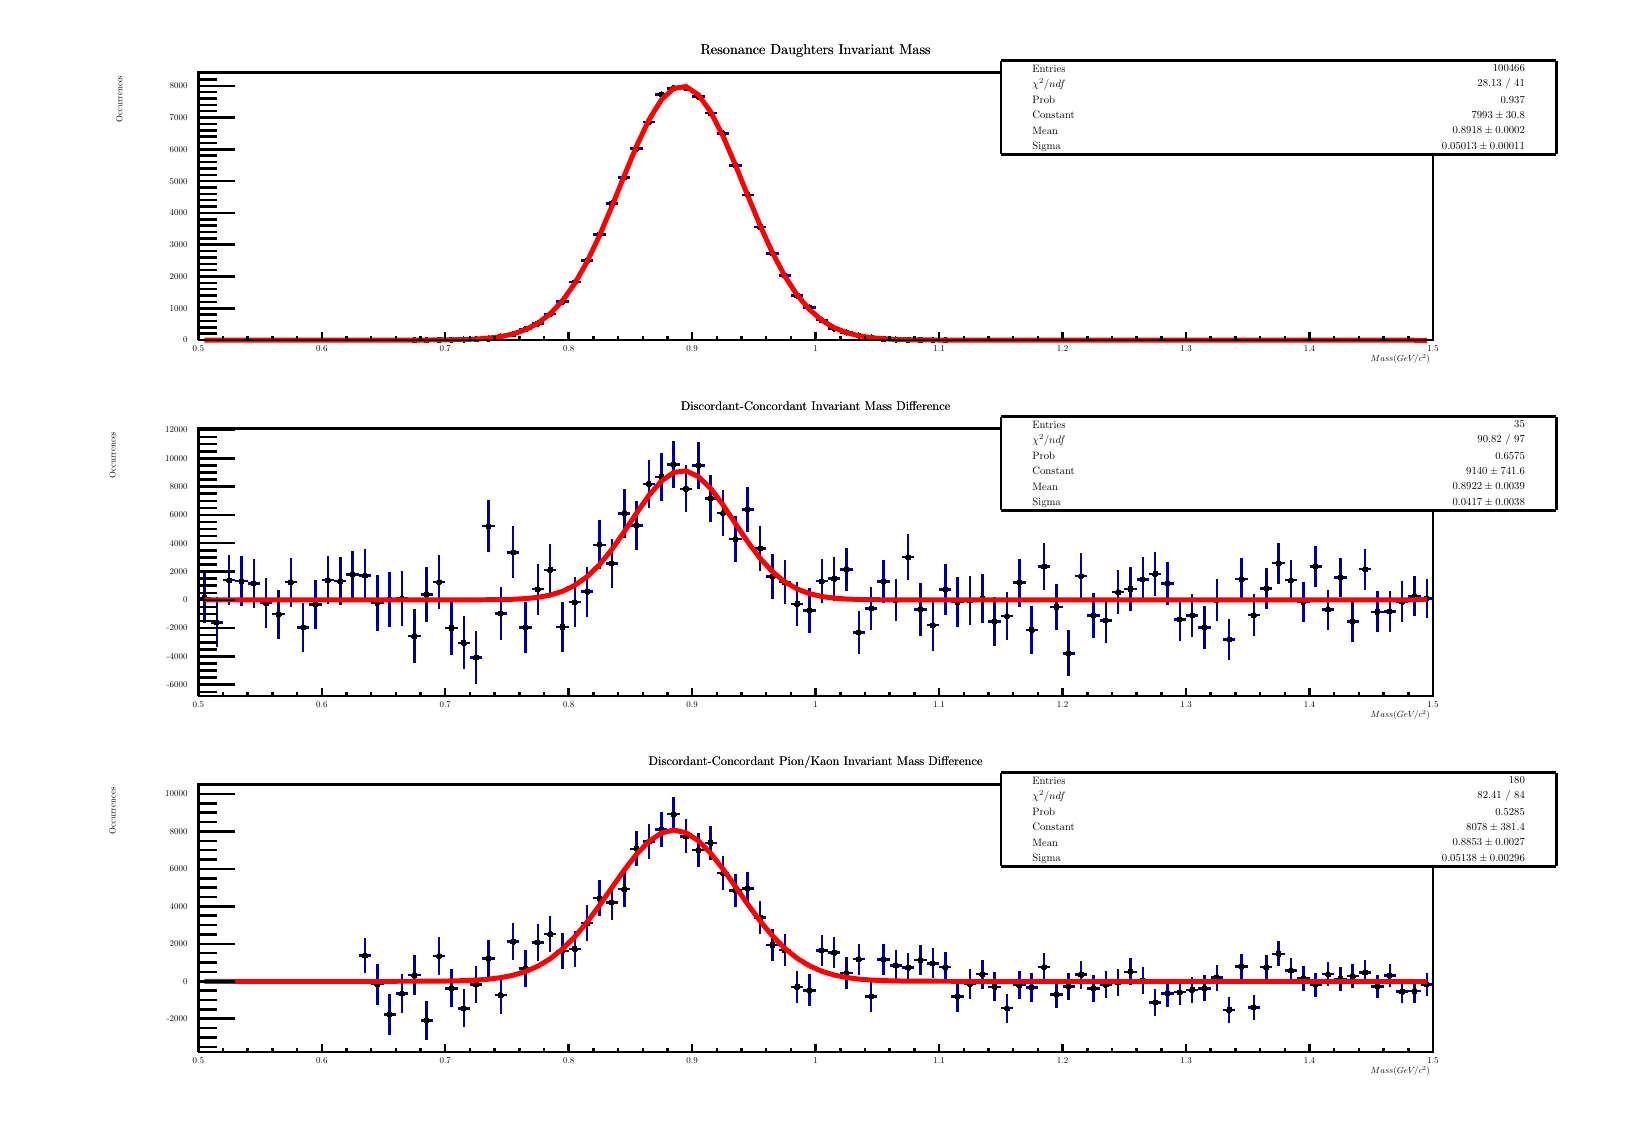
\begin{tikzpicture}
\pgfdeclareplotmark{cross} {
\pgfpathmoveto{\pgfpoint{-0.3\pgfplotmarksize}{\pgfplotmarksize}}
\pgfpathlineto{\pgfpoint{+0.3\pgfplotmarksize}{\pgfplotmarksize}}
\pgfpathlineto{\pgfpoint{+0.3\pgfplotmarksize}{0.3\pgfplotmarksize}}
\pgfpathlineto{\pgfpoint{+1\pgfplotmarksize}{0.3\pgfplotmarksize}}
\pgfpathlineto{\pgfpoint{+1\pgfplotmarksize}{-0.3\pgfplotmarksize}}
\pgfpathlineto{\pgfpoint{+0.3\pgfplotmarksize}{-0.3\pgfplotmarksize}}
\pgfpathlineto{\pgfpoint{+0.3\pgfplotmarksize}{-1.\pgfplotmarksize}}
\pgfpathlineto{\pgfpoint{-0.3\pgfplotmarksize}{-1.\pgfplotmarksize}}
\pgfpathlineto{\pgfpoint{-0.3\pgfplotmarksize}{-0.3\pgfplotmarksize}}
\pgfpathlineto{\pgfpoint{-1.\pgfplotmarksize}{-0.3\pgfplotmarksize}}
\pgfpathlineto{\pgfpoint{-1.\pgfplotmarksize}{0.3\pgfplotmarksize}}
\pgfpathlineto{\pgfpoint{-0.3\pgfplotmarksize}{0.3\pgfplotmarksize}}
\pgfpathclose
\pgfusepathqstroke
}
\pgfdeclareplotmark{cross*} {
\pgfpathmoveto{\pgfpoint{-0.3\pgfplotmarksize}{\pgfplotmarksize}}
\pgfpathlineto{\pgfpoint{+0.3\pgfplotmarksize}{\pgfplotmarksize}}
\pgfpathlineto{\pgfpoint{+0.3\pgfplotmarksize}{0.3\pgfplotmarksize}}
\pgfpathlineto{\pgfpoint{+1\pgfplotmarksize}{0.3\pgfplotmarksize}}
\pgfpathlineto{\pgfpoint{+1\pgfplotmarksize}{-0.3\pgfplotmarksize}}
\pgfpathlineto{\pgfpoint{+0.3\pgfplotmarksize}{-0.3\pgfplotmarksize}}
\pgfpathlineto{\pgfpoint{+0.3\pgfplotmarksize}{-1.\pgfplotmarksize}}
\pgfpathlineto{\pgfpoint{-0.3\pgfplotmarksize}{-1.\pgfplotmarksize}}
\pgfpathlineto{\pgfpoint{-0.3\pgfplotmarksize}{-0.3\pgfplotmarksize}}
\pgfpathlineto{\pgfpoint{-1.\pgfplotmarksize}{-0.3\pgfplotmarksize}}
\pgfpathlineto{\pgfpoint{-1.\pgfplotmarksize}{0.3\pgfplotmarksize}}
\pgfpathlineto{\pgfpoint{-0.3\pgfplotmarksize}{0.3\pgfplotmarksize}}
\pgfpathclose
\pgfusepathqfillstroke
}
\pgfdeclareplotmark{newstar} {
\pgfpathmoveto{\pgfqpoint{0pt}{\pgfplotmarksize}}
\pgfpathlineto{\pgfqpointpolar{44}{0.5\pgfplotmarksize}}
\pgfpathlineto{\pgfqpointpolar{18}{\pgfplotmarksize}}
\pgfpathlineto{\pgfqpointpolar{-20}{0.5\pgfplotmarksize}}
\pgfpathlineto{\pgfqpointpolar{-54}{\pgfplotmarksize}}
\pgfpathlineto{\pgfqpointpolar{-90}{0.5\pgfplotmarksize}}
\pgfpathlineto{\pgfqpointpolar{234}{\pgfplotmarksize}}
\pgfpathlineto{\pgfqpointpolar{198}{0.5\pgfplotmarksize}}
\pgfpathlineto{\pgfqpointpolar{162}{\pgfplotmarksize}}
\pgfpathlineto{\pgfqpointpolar{134}{0.5\pgfplotmarksize}}
\pgfpathclose
\pgfusepathqstroke
}
\pgfdeclareplotmark{newstar*} {
\pgfpathmoveto{\pgfqpoint{0pt}{\pgfplotmarksize}}
\pgfpathlineto{\pgfqpointpolar{44}{0.5\pgfplotmarksize}}
\pgfpathlineto{\pgfqpointpolar{18}{\pgfplotmarksize}}
\pgfpathlineto{\pgfqpointpolar{-20}{0.5\pgfplotmarksize}}
\pgfpathlineto{\pgfqpointpolar{-54}{\pgfplotmarksize}}
\pgfpathlineto{\pgfqpointpolar{-90}{0.5\pgfplotmarksize}}
\pgfpathlineto{\pgfqpointpolar{234}{\pgfplotmarksize}}
\pgfpathlineto{\pgfqpointpolar{198}{0.5\pgfplotmarksize}}
\pgfpathlineto{\pgfqpointpolar{162}{\pgfplotmarksize}}
\pgfpathlineto{\pgfqpointpolar{134}{0.5\pgfplotmarksize}}
\pgfpathclose
\pgfusepathqfillstroke
}
\definecolor{c}{rgb}{1,1,1};
\draw [color=c, fill=c] (0,0) rectangle (20,13.5632);
\draw [color=c, fill=c] (0.2,9.17778) rectangle (19.8,13.4276);
\draw [color=c, fill=c] (2.16,9.60276) rectangle (17.84,13.0026);
\definecolor{c}{rgb}{0,0,0};
\draw [c,line width=0.9] (2.16,9.60276) -- (2.16,13.0026) -- (17.84,13.0026) -- (17.84,9.60276) -- (2.16,9.60276);
\definecolor{c}{rgb}{0,0,0.6};
\draw [c,line width=0.9] (4.904,9.60276) -- (4.904,9.60316);
\draw [c,line width=0.9] (4.904,9.60316) -- (4.904,9.60357);
\draw [c,line width=0.9] (4.8256,9.60316) -- (4.904,9.60316);
\draw [c,line width=0.9] (4.904,9.60316) -- (4.9824,9.60316);
\definecolor{c}{rgb}{0,0,0};
\foreach \P in {(4.904,9.60316)}{\draw[mark options={color=c,fill=c},mark size=2.402402pt, line width=0.000000pt, mark=*,mark size=1pt] plot coordinates {\P};}
\definecolor{c}{rgb}{0,0,0.6};
\draw [c,line width=0.9] (5.0608,9.60299) -- (5.0608,9.60357);
\draw [c,line width=0.9] (5.0608,9.60357) -- (5.0608,9.60414);
\draw [c,line width=0.9] (4.9824,9.60357) -- (5.0608,9.60357);
\draw [c,line width=0.9] (5.0608,9.60357) -- (5.1392,9.60357);
\definecolor{c}{rgb}{0,0,0};
\foreach \P in {(5.0608,9.60357)}{\draw[mark options={color=c,fill=c},mark size=2.402402pt, line width=0.000000pt, mark=*,mark size=1pt] plot coordinates {\P};}
\definecolor{c}{rgb}{0,0,0.6};
\draw [c,line width=0.9] (5.2176,9.60357) -- (5.2176,9.60437);
\draw [c,line width=0.9] (5.2176,9.60437) -- (5.2176,9.60518);
\draw [c,line width=0.9] (5.1392,9.60437) -- (5.2176,9.60437);
\draw [c,line width=0.9] (5.2176,9.60437) -- (5.296,9.60437);
\definecolor{c}{rgb}{0,0,0};
\foreach \P in {(5.2176,9.60437)}{\draw[mark options={color=c,fill=c},mark size=2.402402pt, line width=0.000000pt, mark=*,mark size=1pt] plot coordinates {\P};}
\definecolor{c}{rgb}{0,0,0.6};
\draw [c,line width=0.9] (5.3744,9.60485) -- (5.3744,9.60599);
\draw [c,line width=0.9] (5.3744,9.60599) -- (5.3744,9.60713);
\draw [c,line width=0.9] (5.296,9.60599) -- (5.3744,9.60599);
\draw [c,line width=0.9] (5.3744,9.60599) -- (5.4528,9.60599);
\definecolor{c}{rgb}{0,0,0};
\foreach \P in {(5.3744,9.60599)}{\draw[mark options={color=c,fill=c},mark size=2.402402pt, line width=0.000000pt, mark=*,mark size=1pt] plot coordinates {\P};}
\definecolor{c}{rgb}{0,0,0.6};
\draw [c,line width=0.9] (5.5312,9.60831) -- (5.5312,9.61002);
\draw [c,line width=0.9] (5.5312,9.61002) -- (5.5312,9.61174);
\draw [c,line width=0.9] (5.4528,9.61002) -- (5.5312,9.61002);
\draw [c,line width=0.9] (5.5312,9.61002) -- (5.6096,9.61002);
\definecolor{c}{rgb}{0,0,0};
\foreach \P in {(5.5312,9.61002)}{\draw[mark options={color=c,fill=c},mark size=2.402402pt, line width=0.000000pt, mark=*,mark size=1pt] plot coordinates {\P};}
\definecolor{c}{rgb}{0,0,0.6};
\draw [c,line width=0.9] (5.688,9.61266) -- (5.688,9.61487);
\draw [c,line width=0.9] (5.688,9.61487) -- (5.688,9.61708);
\draw [c,line width=0.9] (5.6096,9.61487) -- (5.688,9.61487);
\draw [c,line width=0.9] (5.688,9.61487) -- (5.7664,9.61487);
\definecolor{c}{rgb}{0,0,0};
\foreach \P in {(5.688,9.61487)}{\draw[mark options={color=c,fill=c},mark size=2.402402pt, line width=0.000000pt, mark=*,mark size=1pt] plot coordinates {\P};}
\definecolor{c}{rgb}{0,0,0.6};
\draw [c,line width=0.9] (5.8448,9.62009) -- (5.8448,9.62294);
\draw [c,line width=0.9] (5.8448,9.62294) -- (5.8448,9.62579);
\draw [c,line width=0.9] (5.7664,9.62294) -- (5.8448,9.62294);
\draw [c,line width=0.9] (5.8448,9.62294) -- (5.9232,9.62294);
\definecolor{c}{rgb}{0,0,0};
\foreach \P in {(5.8448,9.62294)}{\draw[mark options={color=c,fill=c},mark size=2.402402pt, line width=0.000000pt, mark=*,mark size=1pt] plot coordinates {\P};}
\definecolor{c}{rgb}{0,0,0.6};
\draw [c,line width=0.9] (6.0016,9.64254) -- (6.0016,9.64675);
\draw [c,line width=0.9] (6.0016,9.64675) -- (6.0016,9.65097);
\draw [c,line width=0.9] (5.9232,9.64675) -- (6.0016,9.64675);
\draw [c,line width=0.9] (6.0016,9.64675) -- (6.08,9.64675);
\definecolor{c}{rgb}{0,0,0};
\foreach \P in {(6.0016,9.64675)}{\draw[mark options={color=c,fill=c},mark size=2.402402pt, line width=0.000000pt, mark=*,mark size=1pt] plot coordinates {\P};}
\definecolor{c}{rgb}{0,0,0.6};
\draw [c,line width=0.9] (6.1584,9.67155) -- (6.1584,9.67703);
\draw [c,line width=0.9] (6.1584,9.67703) -- (6.1584,9.6825);
\draw [c,line width=0.9] (6.08,9.67703) -- (6.1584,9.67703);
\draw [c,line width=0.9] (6.1584,9.67703) -- (6.2368,9.67703);
\definecolor{c}{rgb}{0,0,0};
\foreach \P in {(6.1584,9.67703)}{\draw[mark options={color=c,fill=c},mark size=2.402402pt, line width=0.000000pt, mark=*,mark size=1pt] plot coordinates {\P};}
\definecolor{c}{rgb}{0,0,0.6};
\draw [c,line width=0.9] (6.3152,9.73451) -- (6.3152,9.74201);
\draw [c,line width=0.9] (6.3152,9.74201) -- (6.3152,9.74951);
\draw [c,line width=0.9] (6.2368,9.74201) -- (6.3152,9.74201);
\draw [c,line width=0.9] (6.3152,9.74201) -- (6.3936,9.74201);
\definecolor{c}{rgb}{0,0,0};
\foreach \P in {(6.3152,9.74201)}{\draw[mark options={color=c,fill=c},mark size=2.402402pt, line width=0.000000pt, mark=*,mark size=1pt] plot coordinates {\P};}
\definecolor{c}{rgb}{0,0,0.6};
\draw [c,line width=0.9] (6.472,9.80581) -- (6.472,9.81507);
\draw [c,line width=0.9] (6.472,9.81507) -- (6.472,9.82433);
\draw [c,line width=0.9] (6.3936,9.81507) -- (6.472,9.81507);
\draw [c,line width=0.9] (6.472,9.81507) -- (6.5504,9.81507);
\definecolor{c}{rgb}{0,0,0};
\foreach \P in {(6.472,9.81507)}{\draw[mark options={color=c,fill=c},mark size=2.402402pt, line width=0.000000pt, mark=*,mark size=1pt] plot coordinates {\P};}
\definecolor{c}{rgb}{0,0,0.6};
\draw [c,line width=0.9] (6.6288,9.92257) -- (6.6288,9.93414);
\draw [c,line width=0.9] (6.6288,9.93414) -- (6.6288,9.9457);
\draw [c,line width=0.9] (6.5504,9.93414) -- (6.6288,9.93414);
\draw [c,line width=0.9] (6.6288,9.93414) -- (6.7072,9.93414);
\definecolor{c}{rgb}{0,0,0};
\foreach \P in {(6.6288,9.93414)}{\draw[mark options={color=c,fill=c},mark size=2.402402pt, line width=0.000000pt, mark=*,mark size=1pt] plot coordinates {\P};}
\definecolor{c}{rgb}{0,0,0.6};
\draw [c,line width=0.9] (6.7856,10.0755) -- (6.7856,10.0895);
\draw [c,line width=0.9] (6.7856,10.0895) -- (6.7856,10.1036);
\draw [c,line width=0.9] (6.7072,10.0895) -- (6.7856,10.0895);
\draw [c,line width=0.9] (6.7856,10.0895) -- (6.864,10.0895);
\definecolor{c}{rgb}{0,0,0};
\foreach \P in {(6.7856,10.0895)}{\draw[mark options={color=c,fill=c},mark size=2.402402pt, line width=0.000000pt, mark=*,mark size=1pt] plot coordinates {\P};}
\definecolor{c}{rgb}{0,0,0.6};
\draw [c,line width=0.9] (6.9424,10.3213) -- (6.9424,10.3386);
\draw [c,line width=0.9] (6.9424,10.3386) -- (6.9424,10.3558);
\draw [c,line width=0.9] (6.864,10.3386) -- (6.9424,10.3386);
\draw [c,line width=0.9] (6.9424,10.3386) -- (7.0208,10.3386);
\definecolor{c}{rgb}{0,0,0};
\foreach \P in {(6.9424,10.3386)}{\draw[mark options={color=c,fill=c},mark size=2.402402pt, line width=0.000000pt, mark=*,mark size=1pt] plot coordinates {\P};}
\definecolor{c}{rgb}{0,0,0.6};
\draw [c,line width=0.9] (7.0992,10.5905) -- (7.0992,10.6106);
\draw [c,line width=0.9] (7.0992,10.6106) -- (7.0992,10.6308);
\draw [c,line width=0.9] (7.0208,10.6106) -- (7.0992,10.6106);
\draw [c,line width=0.9] (7.0992,10.6106) -- (7.1776,10.6106);
\definecolor{c}{rgb}{0,0,0};
\foreach \P in {(7.0992,10.6106)}{\draw[mark options={color=c,fill=c},mark size=2.402402pt, line width=0.000000pt, mark=*,mark size=1pt] plot coordinates {\P};}
\definecolor{c}{rgb}{0,0,0.6};
\draw [c,line width=0.9] (7.256,10.9216) -- (7.256,10.9448);
\draw [c,line width=0.9] (7.256,10.9448) -- (7.256,10.9681);
\draw [c,line width=0.9] (7.1776,10.9448) -- (7.256,10.9448);
\draw [c,line width=0.9] (7.256,10.9448) -- (7.3344,10.9448);
\definecolor{c}{rgb}{0,0,0};
\foreach \P in {(7.256,10.9448)}{\draw[mark options={color=c,fill=c},mark size=2.402402pt, line width=0.000000pt, mark=*,mark size=1pt] plot coordinates {\P};}
\definecolor{c}{rgb}{0,0,0.6};
\draw [c,line width=0.9] (7.4128,11.3083) -- (7.4128,11.3347);
\draw [c,line width=0.9] (7.4128,11.3347) -- (7.4128,11.3612);
\draw [c,line width=0.9] (7.3344,11.3347) -- (7.4128,11.3347);
\draw [c,line width=0.9] (7.4128,11.3347) -- (7.4912,11.3347);
\definecolor{c}{rgb}{0,0,0};
\foreach \P in {(7.4128,11.3347)}{\draw[mark options={color=c,fill=c},mark size=2.402402pt, line width=0.000000pt, mark=*,mark size=1pt] plot coordinates {\P};}
\definecolor{c}{rgb}{0,0,0.6};
\draw [c,line width=0.9] (7.5696,11.6393) -- (7.5696,11.6681);
\draw [c,line width=0.9] (7.5696,11.6681) -- (7.5696,11.697);
\draw [c,line width=0.9] (7.4912,11.6681) -- (7.5696,11.6681);
\draw [c,line width=0.9] (7.5696,11.6681) -- (7.648,11.6681);
\definecolor{c}{rgb}{0,0,0};
\foreach \P in {(7.5696,11.6681)}{\draw[mark options={color=c,fill=c},mark size=2.402402pt, line width=0.000000pt, mark=*,mark size=1pt] plot coordinates {\P};}
\definecolor{c}{rgb}{0,0,0.6};
\draw [c,line width=0.9] (7.7264,12.0037) -- (7.7264,12.035);
\draw [c,line width=0.9] (7.7264,12.035) -- (7.7264,12.0664);
\draw [c,line width=0.9] (7.648,12.035) -- (7.7264,12.035);
\draw [c,line width=0.9] (7.7264,12.035) -- (7.8048,12.035);
\definecolor{c}{rgb}{0,0,0};
\foreach \P in {(7.7264,12.035)}{\draw[mark options={color=c,fill=c},mark size=2.402402pt, line width=0.000000pt, mark=*,mark size=1pt] plot coordinates {\P};}
\definecolor{c}{rgb}{0,0,0.6};
\draw [c,line width=0.9] (7.8832,12.3382) -- (7.8832,12.3717);
\draw [c,line width=0.9] (7.8832,12.3717) -- (7.8832,12.4051);
\draw [c,line width=0.9] (7.8048,12.3717) -- (7.8832,12.3717);
\draw [c,line width=0.9] (7.8832,12.3717) -- (7.9616,12.3717);
\definecolor{c}{rgb}{0,0,0};
\foreach \P in {(7.8832,12.3717)}{\draw[mark options={color=c,fill=c},mark size=2.402402pt, line width=0.000000pt, mark=*,mark size=1pt] plot coordinates {\P};}
\definecolor{c}{rgb}{0,0,0.6};
\draw [c,line width=0.9] (8.04,12.6829) -- (8.04,12.7184);
\draw [c,line width=0.9] (8.04,12.7184) -- (8.04,12.7538);
\draw [c,line width=0.9] (7.9616,12.7184) -- (8.04,12.7184);
\draw [c,line width=0.9] (8.04,12.7184) -- (8.1184,12.7184);
\definecolor{c}{rgb}{0,0,0};
\foreach \P in {(8.04,12.7184)}{\draw[mark options={color=c,fill=c},mark size=2.402402pt, line width=0.000000pt, mark=*,mark size=1pt] plot coordinates {\P};}
\definecolor{c}{rgb}{0,0,0.6};
\draw [c,line width=0.9] (8.1968,12.764) -- (8.1968,12.7999);
\draw [c,line width=0.9] (8.1968,12.7999) -- (8.1968,12.8358);
\draw [c,line width=0.9] (8.1184,12.7999) -- (8.1968,12.7999);
\draw [c,line width=0.9] (8.1968,12.7999) -- (8.2752,12.7999);
\definecolor{c}{rgb}{0,0,0};
\foreach \P in {(8.1968,12.7999)}{\draw[mark options={color=c,fill=c},mark size=2.402402pt, line width=0.000000pt, mark=*,mark size=1pt] plot coordinates {\P};}
\definecolor{c}{rgb}{0,0,0.6};
\draw [c,line width=0.9] (8.3536,12.7688) -- (8.3536,12.8048);
\draw [c,line width=0.9] (8.3536,12.8048) -- (8.3536,12.8407);
\draw [c,line width=0.9] (8.2752,12.8048) -- (8.3536,12.8048);
\draw [c,line width=0.9] (8.3536,12.8048) -- (8.432,12.8048);
\definecolor{c}{rgb}{0,0,0};
\foreach \P in {(8.3536,12.8048)}{\draw[mark options={color=c,fill=c},mark size=2.402402pt, line width=0.000000pt, mark=*,mark size=1pt] plot coordinates {\P};}
\definecolor{c}{rgb}{0,0,0.6};
\draw [c,line width=0.9] (8.5104,12.6596) -- (8.5104,12.695);
\draw [c,line width=0.9] (8.5104,12.695) -- (8.5104,12.7303);
\draw [c,line width=0.9] (8.432,12.695) -- (8.5104,12.695);
\draw [c,line width=0.9] (8.5104,12.695) -- (8.5888,12.695);
\definecolor{c}{rgb}{0,0,0};
\foreach \P in {(8.5104,12.695)}{\draw[mark options={color=c,fill=c},mark size=2.402402pt, line width=0.000000pt, mark=*,mark size=1pt] plot coordinates {\P};}
\definecolor{c}{rgb}{0,0,0.6};
\draw [c,line width=0.9] (8.6672,12.4506) -- (8.6672,12.4847);
\draw [c,line width=0.9] (8.6672,12.4847) -- (8.6672,12.5188);
\draw [c,line width=0.9] (8.5888,12.4847) -- (8.6672,12.4847);
\draw [c,line width=0.9] (8.6672,12.4847) -- (8.7456,12.4847);
\definecolor{c}{rgb}{0,0,0};
\foreach \P in {(8.6672,12.4847)}{\draw[mark options={color=c,fill=c},mark size=2.402402pt, line width=0.000000pt, mark=*,mark size=1pt] plot coordinates {\P};}
\definecolor{c}{rgb}{0,0,0.6};
\draw [c,line width=0.9] (8.824,12.1958) -- (8.824,12.2284);
\draw [c,line width=0.9] (8.824,12.2284) -- (8.824,12.2609);
\draw [c,line width=0.9] (8.7456,12.2284) -- (8.824,12.2284);
\draw [c,line width=0.9] (8.824,12.2284) -- (8.9024,12.2284);
\definecolor{c}{rgb}{0,0,0};
\foreach \P in {(8.824,12.2284)}{\draw[mark options={color=c,fill=c},mark size=2.402402pt, line width=0.000000pt, mark=*,mark size=1pt] plot coordinates {\P};}
\definecolor{c}{rgb}{0,0,0.6};
\draw [c,line width=0.9] (8.9808,11.7928) -- (8.9808,11.8227);
\draw [c,line width=0.9] (8.9808,11.8227) -- (8.9808,11.8527);
\draw [c,line width=0.9] (8.9024,11.8227) -- (8.9808,11.8227);
\draw [c,line width=0.9] (8.9808,11.8227) -- (9.0592,11.8227);
\definecolor{c}{rgb}{0,0,0};
\foreach \P in {(8.9808,11.8227)}{\draw[mark options={color=c,fill=c},mark size=2.402402pt, line width=0.000000pt, mark=*,mark size=1pt] plot coordinates {\P};}
\definecolor{c}{rgb}{0,0,0.6};
\draw [c,line width=0.9] (9.1376,11.4209) -- (9.1376,11.4482);
\draw [c,line width=0.9] (9.1376,11.4482) -- (9.1376,11.4754);
\draw [c,line width=0.9] (9.0592,11.4482) -- (9.1376,11.4482);
\draw [c,line width=0.9] (9.1376,11.4482) -- (9.216,11.4482);
\definecolor{c}{rgb}{0,0,0};
\foreach \P in {(9.1376,11.4482)}{\draw[mark options={color=c,fill=c},mark size=2.402402pt, line width=0.000000pt, mark=*,mark size=1pt] plot coordinates {\P};}
\definecolor{c}{rgb}{0,0,0.6};
\draw [c,line width=0.9] (9.2944,11.0156) -- (9.2944,11.0397);
\draw [c,line width=0.9] (9.2944,11.0397) -- (9.2944,11.0638);
\draw [c,line width=0.9] (9.216,11.0397) -- (9.2944,11.0397);
\draw [c,line width=0.9] (9.2944,11.0397) -- (9.3728,11.0397);
\definecolor{c}{rgb}{0,0,0};
\foreach \P in {(9.2944,11.0397)}{\draw[mark options={color=c,fill=c},mark size=2.402402pt, line width=0.000000pt, mark=*,mark size=1pt] plot coordinates {\P};}
\definecolor{c}{rgb}{0,0,0.6};
\draw [c,line width=0.9] (9.4512,10.6828) -- (9.4512,10.7039);
\draw [c,line width=0.9] (9.4512,10.7039) -- (9.4512,10.7249);
\draw [c,line width=0.9] (9.3728,10.7039) -- (9.4512,10.7039);
\draw [c,line width=0.9] (9.4512,10.7039) -- (9.5296,10.7039);
\definecolor{c}{rgb}{0,0,0};
\foreach \P in {(9.4512,10.7039)}{\draw[mark options={color=c,fill=c},mark size=2.402402pt, line width=0.000000pt, mark=*,mark size=1pt] plot coordinates {\P};}
\definecolor{c}{rgb}{0,0,0.6};
\draw [c,line width=0.9] (9.608,10.4047) -- (9.608,10.4229);
\draw [c,line width=0.9] (9.608,10.4229) -- (9.608,10.4411);
\draw [c,line width=0.9] (9.5296,10.4229) -- (9.608,10.4229);
\draw [c,line width=0.9] (9.608,10.4229) -- (9.6864,10.4229);
\definecolor{c}{rgb}{0,0,0};
\foreach \P in {(9.608,10.4229)}{\draw[mark options={color=c,fill=c},mark size=2.402402pt, line width=0.000000pt, mark=*,mark size=1pt] plot coordinates {\P};}
\definecolor{c}{rgb}{0,0,0.6};
\draw [c,line width=0.9] (9.7648,10.1535) -- (9.7648,10.1686);
\draw [c,line width=0.9] (9.7648,10.1686) -- (9.7648,10.1838);
\draw [c,line width=0.9] (9.6864,10.1686) -- (9.7648,10.1686);
\draw [c,line width=0.9] (9.7648,10.1686) -- (9.8432,10.1686);
\definecolor{c}{rgb}{0,0,0};
\foreach \P in {(9.7648,10.1686)}{\draw[mark options={color=c,fill=c},mark size=2.402402pt, line width=0.000000pt, mark=*,mark size=1pt] plot coordinates {\P};}
\definecolor{c}{rgb}{0,0,0.6};
\draw [c,line width=0.9] (9.9216,10.0028) -- (9.9216,10.0157);
\draw [c,line width=0.9] (9.9216,10.0157) -- (9.9216,10.0286);
\draw [c,line width=0.9] (9.8432,10.0157) -- (9.9216,10.0157);
\draw [c,line width=0.9] (9.9216,10.0157) -- (10,10.0157);
\definecolor{c}{rgb}{0,0,0};
\foreach \P in {(9.9216,10.0157)}{\draw[mark options={color=c,fill=c},mark size=2.402402pt, line width=0.000000pt, mark=*,mark size=1pt] plot coordinates {\P};}
\definecolor{c}{rgb}{0,0,0.6};
\draw [c,line width=0.9] (10.0784,9.84454) -- (10.0784,9.85462);
\draw [c,line width=0.9] (10.0784,9.85462) -- (10.0784,9.86471);
\draw [c,line width=0.9] (10,9.85462) -- (10.0784,9.85462);
\draw [c,line width=0.9] (10.0784,9.85462) -- (10.1568,9.85462);
\definecolor{c}{rgb}{0,0,0};
\foreach \P in {(10.0784,9.85462)}{\draw[mark options={color=c,fill=c},mark size=2.402402pt, line width=0.000000pt, mark=*,mark size=1pt] plot coordinates {\P};}
\definecolor{c}{rgb}{0,0,0.6};
\draw [c,line width=0.9] (10.2352,9.74394) -- (10.2352,9.7517);
\draw [c,line width=0.9] (10.2352,9.7517) -- (10.2352,9.75945);
\draw [c,line width=0.9] (10.1568,9.7517) -- (10.2352,9.7517);
\draw [c,line width=0.9] (10.2352,9.7517) -- (10.3136,9.7517);
\definecolor{c}{rgb}{0,0,0};
\foreach \P in {(10.2352,9.7517)}{\draw[mark options={color=c,fill=c},mark size=2.402402pt, line width=0.000000pt, mark=*,mark size=1pt] plot coordinates {\P};}
\definecolor{c}{rgb}{0,0,0.6};
\draw [c,line width=0.9] (10.392,9.69455) -- (10.392,9.70084);
\draw [c,line width=0.9] (10.392,9.70084) -- (10.392,9.70713);
\draw [c,line width=0.9] (10.3136,9.70084) -- (10.392,9.70084);
\draw [c,line width=0.9] (10.392,9.70084) -- (10.4704,9.70084);
\definecolor{c}{rgb}{0,0,0};
\foreach \P in {(10.392,9.70084)}{\draw[mark options={color=c,fill=c},mark size=2.402402pt, line width=0.000000pt, mark=*,mark size=1pt] plot coordinates {\P};}
\definecolor{c}{rgb}{0,0,0.6};
\draw [c,line width=0.9] (10.5488,9.65604) -- (10.5488,9.66088);
\draw [c,line width=0.9] (10.5488,9.66088) -- (10.5488,9.66572);
\draw [c,line width=0.9] (10.4704,9.66088) -- (10.5488,9.66088);
\draw [c,line width=0.9] (10.5488,9.66088) -- (10.6272,9.66088);
\definecolor{c}{rgb}{0,0,0};
\foreach \P in {(10.5488,9.66088)}{\draw[mark options={color=c,fill=c},mark size=2.402402pt, line width=0.000000pt, mark=*,mark size=1pt] plot coordinates {\P};}
\definecolor{c}{rgb}{0,0,0.6};
\draw [c,line width=0.9] (10.7056,9.62992) -- (10.7056,9.63343);
\draw [c,line width=0.9] (10.7056,9.63343) -- (10.7056,9.63695);
\draw [c,line width=0.9] (10.6272,9.63343) -- (10.7056,9.63343);
\draw [c,line width=0.9] (10.7056,9.63343) -- (10.784,9.63343);
\definecolor{c}{rgb}{0,0,0};
\foreach \P in {(10.7056,9.63343)}{\draw[mark options={color=c,fill=c},mark size=2.402402pt, line width=0.000000pt, mark=*,mark size=1pt] plot coordinates {\P};}
\definecolor{c}{rgb}{0,0,0.6};
\draw [c,line width=0.9] (10.8624,9.6145) -- (10.8624,9.61689);
\draw [c,line width=0.9] (10.8624,9.61689) -- (10.8624,9.61927);
\draw [c,line width=0.9] (10.784,9.61689) -- (10.8624,9.61689);
\draw [c,line width=0.9] (10.8624,9.61689) -- (10.9408,9.61689);
\definecolor{c}{rgb}{0,0,0};
\foreach \P in {(10.8624,9.61689)}{\draw[mark options={color=c,fill=c},mark size=2.402402pt, line width=0.000000pt, mark=*,mark size=1pt] plot coordinates {\P};}
\definecolor{c}{rgb}{0,0,0.6};
\draw [c,line width=0.9] (11.0192,9.60939) -- (11.0192,9.61123);
\draw [c,line width=0.9] (11.0192,9.61123) -- (11.0192,9.61308);
\draw [c,line width=0.9] (10.9408,9.61123) -- (11.0192,9.61123);
\draw [c,line width=0.9] (11.0192,9.61123) -- (11.0976,9.61123);
\definecolor{c}{rgb}{0,0,0};
\foreach \P in {(11.0192,9.61123)}{\draw[mark options={color=c,fill=c},mark size=2.402402pt, line width=0.000000pt, mark=*,mark size=1pt] plot coordinates {\P};}
\definecolor{c}{rgb}{0,0,0.6};
\draw [c,line width=0.9] (11.176,9.60419) -- (11.176,9.60518);
\draw [c,line width=0.9] (11.176,9.60518) -- (11.176,9.60617);
\draw [c,line width=0.9] (11.0976,9.60518) -- (11.176,9.60518);
\draw [c,line width=0.9] (11.176,9.60518) -- (11.2544,9.60518);
\definecolor{c}{rgb}{0,0,0};
\foreach \P in {(11.176,9.60518)}{\draw[mark options={color=c,fill=c},mark size=2.402402pt, line width=0.000000pt, mark=*,mark size=1pt] plot coordinates {\P};}
\definecolor{c}{rgb}{0,0,0.6};
\draw [c,line width=0.9] (11.3328,9.60357) -- (11.3328,9.60437);
\draw [c,line width=0.9] (11.3328,9.60437) -- (11.3328,9.60518);
\draw [c,line width=0.9] (11.2544,9.60437) -- (11.3328,9.60437);
\draw [c,line width=0.9] (11.3328,9.60437) -- (11.4112,9.60437);
\definecolor{c}{rgb}{0,0,0};
\foreach \P in {(11.3328,9.60437)}{\draw[mark options={color=c,fill=c},mark size=2.402402pt, line width=0.000000pt, mark=*,mark size=1pt] plot coordinates {\P};}
\definecolor{c}{rgb}{0,0,0.6};
\draw [c,line width=0.9] (11.4896,9.60299) -- (11.4896,9.60357);
\draw [c,line width=0.9] (11.4896,9.60357) -- (11.4896,9.60414);
\draw [c,line width=0.9] (11.4112,9.60357) -- (11.4896,9.60357);
\draw [c,line width=0.9] (11.4896,9.60357) -- (11.568,9.60357);
\definecolor{c}{rgb}{0,0,0};
\foreach \P in {(11.4896,9.60357)}{\draw[mark options={color=c,fill=c},mark size=2.402402pt, line width=0.000000pt, mark=*,mark size=1pt] plot coordinates {\P};}
\definecolor{c}{rgb}{0,0,0.6};
\draw [c,line width=0.9] (11.6464,9.60327) -- (11.6464,9.60397);
\draw [c,line width=0.9] (11.6464,9.60397) -- (11.6464,9.60467);
\draw [c,line width=0.9] (11.568,9.60397) -- (11.6464,9.60397);
\draw [c,line width=0.9] (11.6464,9.60397) -- (11.7248,9.60397);
\definecolor{c}{rgb}{0,0,0};
\foreach \P in {(11.6464,9.60397)}{\draw[mark options={color=c,fill=c},mark size=2.402402pt, line width=0.000000pt, mark=*,mark size=1pt] plot coordinates {\P};}
\definecolor{c}{rgb}{1,0,0};
\draw [c,line width=1.8] (2.2384,9.60276) -- (2.3952,9.60276) -- (2.552,9.60276) -- (2.7088,9.60276) -- (2.8656,9.60276) -- (3.0224,9.60276) -- (3.1792,9.60276) -- (3.336,9.60276) -- (3.4928,9.60276) -- (3.6496,9.60276) -- (3.8064,9.60276) --
 (3.9632,9.60276) -- (4.12,9.60276) -- (4.2768,9.60276) -- (4.4336,9.60276) -- (4.5904,9.60276) -- (4.7472,9.60276) -- (4.904,9.60276) -- (5.0608,9.60341) -- (5.2176,9.60421) -- (5.3744,9.60588) -- (5.5312,9.6092) -- (5.688,9.61551) --
 (5.8448,9.62703) -- (6.0016,9.64716) -- (6.1584,9.68081) -- (6.3152,9.73461) -- (6.472,9.81681) -- (6.6288,9.9367) -- (6.7856,10.1034) -- (6.9424,10.3241) -- (7.0992,10.6015) -- (7.256,10.9316) -- (7.4128,11.3018) -- (7.5696,11.6905) --
 (7.7264,12.068) -- (7.8832,12.4002) -- (8.04,12.6534) -- (8.1968,12.7997) -- (8.3536,12.8223) -- (8.5104,12.7185) -- (8.6672,12.5005) -- (8.824,12.1927) -- (8.9808,11.8272) -- (9.1376,11.4388) -- (9.2944,11.059) -- (9.4512,10.7128) --
 (9.608,10.4159) -- (9.7648,10.1751) -- (9.9216,9.98996);
\draw [c,line width=1.8] (9.9216,9.98996) -- (10.0784,9.85447) -- (10.2352,9.76001) -- (10.392,9.69716) -- (10.5488,9.65722) -- (10.7056,9.63296) -- (10.8624,9.61885) -- (11.0192,9.611) -- (11.176,9.60681) -- (11.3328,9.60468) -- (11.4896,9.60363) --
 (11.6464,9.60314) -- (11.8032,9.60276) -- (11.96,9.60276) -- (12.1168,9.60276) -- (12.2736,9.60276) -- (12.4304,9.60276) -- (12.5872,9.60276) -- (12.744,9.60276) -- (12.9008,9.60276) -- (13.0576,9.60276) -- (13.2144,9.60276) -- (13.3712,9.60276) --
 (13.528,9.60276) -- (13.6848,9.60276) -- (13.8416,9.60276) -- (13.9984,9.60276) -- (14.1552,9.60276) -- (14.312,9.60276) -- (14.4688,9.60276) -- (14.6256,9.60276) -- (14.7824,9.60276) -- (14.9392,9.60276) -- (15.096,9.60276) -- (15.2528,9.60276) --
 (15.4096,9.60276) -- (15.5664,9.60276) -- (15.7232,9.60276) -- (15.88,9.60276) -- (16.0368,9.60276) -- (16.1936,9.60276) -- (16.3504,9.60276) -- (16.5072,9.60276) -- (16.664,9.60276) -- (16.8208,9.60276) -- (16.9776,9.60276) -- (17.1344,9.60276) --
 (17.2912,9.60276) -- (17.448,9.60276) -- (17.6048,9.60276);
\draw [c,line width=1.8] (17.6048,9.60276) -- (17.7616,9.60276);
\definecolor{c}{rgb}{0,0,0};
\draw [c,line width=0.9] (2.16,9.60276) -- (17.84,9.60276);
\draw [c,line width=0.9] (2.16,9.70475) -- (2.16,9.60276);
\draw [c,line width=0.9] (2.4736,9.65376) -- (2.4736,9.60276);
\draw [c,line width=0.9] (2.7872,9.65376) -- (2.7872,9.60276);
\draw [c,line width=0.9] (3.1008,9.65376) -- (3.1008,9.60276);
\draw [c,line width=0.9] (3.4144,9.65376) -- (3.4144,9.60276);
\draw [c,line width=0.9] (3.728,9.70475) -- (3.728,9.60276);
\draw [c,line width=0.9] (4.0416,9.65376) -- (4.0416,9.60276);
\draw [c,line width=0.9] (4.3552,9.65376) -- (4.3552,9.60276);
\draw [c,line width=0.9] (4.6688,9.65376) -- (4.6688,9.60276);
\draw [c,line width=0.9] (4.9824,9.65376) -- (4.9824,9.60276);
\draw [c,line width=0.9] (5.296,9.70475) -- (5.296,9.60276);
\draw [c,line width=0.9] (5.6096,9.65376) -- (5.6096,9.60276);
\draw [c,line width=0.9] (5.9232,9.65376) -- (5.9232,9.60276);
\draw [c,line width=0.9] (6.2368,9.65376) -- (6.2368,9.60276);
\draw [c,line width=0.9] (6.5504,9.65376) -- (6.5504,9.60276);
\draw [c,line width=0.9] (6.864,9.70475) -- (6.864,9.60276);
\draw [c,line width=0.9] (7.1776,9.65376) -- (7.1776,9.60276);
\draw [c,line width=0.9] (7.4912,9.65376) -- (7.4912,9.60276);
\draw [c,line width=0.9] (7.8048,9.65376) -- (7.8048,9.60276);
\draw [c,line width=0.9] (8.1184,9.65376) -- (8.1184,9.60276);
\draw [c,line width=0.9] (8.432,9.70475) -- (8.432,9.60276);
\draw [c,line width=0.9] (8.7456,9.65376) -- (8.7456,9.60276);
\draw [c,line width=0.9] (9.0592,9.65376) -- (9.0592,9.60276);
\draw [c,line width=0.9] (9.3728,9.65376) -- (9.3728,9.60276);
\draw [c,line width=0.9] (9.6864,9.65376) -- (9.6864,9.60276);
\draw [c,line width=0.9] (10,9.70475) -- (10,9.60276);
\draw [c,line width=0.9] (10.3136,9.65376) -- (10.3136,9.60276);
\draw [c,line width=0.9] (10.6272,9.65376) -- (10.6272,9.60276);
\draw [c,line width=0.9] (10.9408,9.65376) -- (10.9408,9.60276);
\draw [c,line width=0.9] (11.2544,9.65376) -- (11.2544,9.60276);
\draw [c,line width=0.9] (11.568,9.70475) -- (11.568,9.60276);
\draw [c,line width=0.9] (11.8816,9.65376) -- (11.8816,9.60276);
\draw [c,line width=0.9] (12.1952,9.65376) -- (12.1952,9.60276);
\draw [c,line width=0.9] (12.5088,9.65376) -- (12.5088,9.60276);
\draw [c,line width=0.9] (12.8224,9.65376) -- (12.8224,9.60276);
\draw [c,line width=0.9] (13.136,9.70475) -- (13.136,9.60276);
\draw [c,line width=0.9] (13.4496,9.65376) -- (13.4496,9.60276);
\draw [c,line width=0.9] (13.7632,9.65376) -- (13.7632,9.60276);
\draw [c,line width=0.9] (14.0768,9.65376) -- (14.0768,9.60276);
\draw [c,line width=0.9] (14.3904,9.65376) -- (14.3904,9.60276);
\draw [c,line width=0.9] (14.704,9.70475) -- (14.704,9.60276);
\draw [c,line width=0.9] (15.0176,9.65376) -- (15.0176,9.60276);
\draw [c,line width=0.9] (15.3312,9.65376) -- (15.3312,9.60276);
\draw [c,line width=0.9] (15.6448,9.65376) -- (15.6448,9.60276);
\draw [c,line width=0.9] (15.9584,9.65376) -- (15.9584,9.60276);
\draw [c,line width=0.9] (16.272,9.70475) -- (16.272,9.60276);
\draw [c,line width=0.9] (16.5856,9.65376) -- (16.5856,9.60276);
\draw [c,line width=0.9] (16.8992,9.65376) -- (16.8992,9.60276);
\draw [c,line width=0.9] (17.2128,9.65376) -- (17.2128,9.60276);
\draw [c,line width=0.9] (17.5264,9.65376) -- (17.5264,9.60276);
\draw [c,line width=0.9] (17.84,9.70475) -- (17.84,9.60276);
\draw [anchor=base] (2.16,9.46251) node[scale=0.321044, color=c, rotate=0]{0.5};
\draw [anchor=base] (3.728,9.46251) node[scale=0.321044, color=c, rotate=0]{0.6};
\draw [anchor=base] (5.296,9.46251) node[scale=0.321044, color=c, rotate=0]{0.7};
\draw [anchor=base] (6.864,9.46251) node[scale=0.321044, color=c, rotate=0]{0.8};
\draw [anchor=base] (8.432,9.46251) node[scale=0.321044, color=c, rotate=0]{0.9};
\draw [anchor=base] (10,9.46251) node[scale=0.321044, color=c, rotate=0]{1};
\draw [anchor=base] (11.568,9.46251) node[scale=0.321044, color=c, rotate=0]{1.1};
\draw [anchor=base] (13.136,9.46251) node[scale=0.321044, color=c, rotate=0]{1.2};
\draw [anchor=base] (14.704,9.46251) node[scale=0.321044, color=c, rotate=0]{1.3};
\draw [anchor=base] (16.272,9.46251) node[scale=0.321044, color=c, rotate=0]{1.4};
\draw [anchor=base] (17.84,9.46251) node[scale=0.321044, color=c, rotate=0]{1.5};
\draw [anchor= east] (17.84,9.36477) node[scale=0.321044, color=c, rotate=0]{$Mass (GeV/c^{2})$};
\draw [c,line width=0.9] (2.16,9.60276) -- (2.16,13.0026);
\draw [c,line width=0.9] (2.6304,9.60276) -- (2.16,9.60276);
\draw [c,line width=0.9] (2.3952,9.68348) -- (2.16,9.68348);
\draw [c,line width=0.9] (2.3952,9.76421) -- (2.16,9.76421);
\draw [c,line width=0.9] (2.3952,9.84494) -- (2.16,9.84494);
\draw [c,line width=0.9] (2.3952,9.92566) -- (2.16,9.92566);
\draw [c,line width=0.9] (2.6304,10.0064) -- (2.16,10.0064);
\draw [c,line width=0.9] (2.3952,10.0871) -- (2.16,10.0871);
\draw [c,line width=0.9] (2.3952,10.1678) -- (2.16,10.1678);
\draw [c,line width=0.9] (2.3952,10.2486) -- (2.16,10.2486);
\draw [c,line width=0.9] (2.3952,10.3293) -- (2.16,10.3293);
\draw [c,line width=0.9] (2.6304,10.41) -- (2.16,10.41);
\draw [c,line width=0.9] (2.3952,10.4907) -- (2.16,10.4907);
\draw [c,line width=0.9] (2.3952,10.5715) -- (2.16,10.5715);
\draw [c,line width=0.9] (2.3952,10.6522) -- (2.16,10.6522);
\draw [c,line width=0.9] (2.3952,10.7329) -- (2.16,10.7329);
\draw [c,line width=0.9] (2.6304,10.8136) -- (2.16,10.8136);
\draw [c,line width=0.9] (2.3952,10.8944) -- (2.16,10.8944);
\draw [c,line width=0.9] (2.3952,10.9751) -- (2.16,10.9751);
\draw [c,line width=0.9] (2.3952,11.0558) -- (2.16,11.0558);
\draw [c,line width=0.9] (2.3952,11.1366) -- (2.16,11.1366);
\draw [c,line width=0.9] (2.6304,11.2173) -- (2.16,11.2173);
\draw [c,line width=0.9] (2.3952,11.298) -- (2.16,11.298);
\draw [c,line width=0.9] (2.3952,11.3787) -- (2.16,11.3787);
\draw [c,line width=0.9] (2.3952,11.4595) -- (2.16,11.4595);
\draw [c,line width=0.9] (2.3952,11.5402) -- (2.16,11.5402);
\draw [c,line width=0.9] (2.6304,11.6209) -- (2.16,11.6209);
\draw [c,line width=0.9] (2.3952,11.7016) -- (2.16,11.7016);
\draw [c,line width=0.9] (2.3952,11.7824) -- (2.16,11.7824);
\draw [c,line width=0.9] (2.3952,11.8631) -- (2.16,11.8631);
\draw [c,line width=0.9] (2.3952,11.9438) -- (2.16,11.9438);
\draw [c,line width=0.9] (2.6304,12.0245) -- (2.16,12.0245);
\draw [c,line width=0.9] (2.3952,12.1053) -- (2.16,12.1053);
\draw [c,line width=0.9] (2.3952,12.186) -- (2.16,12.186);
\draw [c,line width=0.9] (2.3952,12.2667) -- (2.16,12.2667);
\draw [c,line width=0.9] (2.3952,12.3474) -- (2.16,12.3474);
\draw [c,line width=0.9] (2.6304,12.4282) -- (2.16,12.4282);
\draw [c,line width=0.9] (2.3952,12.5089) -- (2.16,12.5089);
\draw [c,line width=0.9] (2.3952,12.5896) -- (2.16,12.5896);
\draw [c,line width=0.9] (2.3952,12.6703) -- (2.16,12.6703);
\draw [c,line width=0.9] (2.3952,12.7511) -- (2.16,12.7511);
\draw [c,line width=0.9] (2.6304,12.8318) -- (2.16,12.8318);
\draw [c,line width=0.9] (2.6304,12.8318) -- (2.16,12.8318);
\draw [c,line width=0.9] (2.3952,12.9125) -- (2.16,12.9125);
\draw [c,line width=0.9] (2.3952,12.9933) -- (2.16,12.9933);
\draw [anchor= east] (2.062,9.60276) node[scale=0.321044, color=c, rotate=0]{0};
\draw [anchor= east] (2.062,10.0064) node[scale=0.321044, color=c, rotate=0]{1000};
\draw [anchor= east] (2.062,10.41) node[scale=0.321044, color=c, rotate=0]{2000};
\draw [anchor= east] (2.062,10.8136) node[scale=0.321044, color=c, rotate=0]{3000};
\draw [anchor= east] (2.062,11.2173) node[scale=0.321044, color=c, rotate=0]{4000};
\draw [anchor= east] (2.062,11.6209) node[scale=0.321044, color=c, rotate=0]{5000};
\draw [anchor= east] (2.062,12.0245) node[scale=0.321044, color=c, rotate=0]{6000};
\draw [anchor= east] (2.062,12.4282) node[scale=0.321044, color=c, rotate=0]{7000};
\draw [anchor= east] (2.062,12.8318) node[scale=0.321044, color=c, rotate=0]{8000};
\draw [anchor= east] (1.15791,13.0026) node[scale=0.321044, color=c, rotate=90]{Occurrences};
\draw (10,13.2684) node[scale=0.513671, color=c, rotate=0]{Resonance Daughters Invariant Mass};
\definecolor{c}{rgb}{1,1,1};
\draw [color=c, fill=c] (12.352,11.9614) rectangle (19.408,13.1513);
\definecolor{c}{rgb}{0,0,0};
\draw [c,line width=0.9] (12.352,11.9614) -- (19.408,11.9614);
\draw [c,line width=0.9] (19.408,11.9614) -- (19.408,13.1513);
\draw [c,line width=0.9] (19.408,13.1513) -- (12.352,13.1513);
\draw [c,line width=0.9] (12.352,13.1513) -- (12.352,11.9614);
\draw [anchor= west] (12.7048,13.0522) node[scale=0.385253, color=c, rotate=0]{Entries };
\draw [anchor= east] (19.0552,13.0522) node[scale=0.385253, color=c, rotate=0]{ 100466};
\draw [anchor= west] (12.7048,12.8539) node[scale=0.385253, color=c, rotate=0]{$\chi^{2} / ndf $};
\draw [anchor= east] (19.0552,12.8539) node[scale=0.385253, color=c, rotate=0]{ 28.13 / 41};
\draw [anchor= west] (12.7048,12.6555) node[scale=0.385253, color=c, rotate=0]{Prob  };
\draw [anchor= east] (19.0552,12.6555) node[scale=0.385253, color=c, rotate=0]{ 0.937};
\draw [anchor= west] (12.7048,12.4572) node[scale=0.385253, color=c, rotate=0]{Constant };
\draw [anchor= east] (19.0552,12.4572) node[scale=0.385253, color=c, rotate=0]{$  7993 \pm 30.8$};
\draw [anchor= west] (12.7048,12.2589) node[scale=0.385253, color=c, rotate=0]{Mean     };
\draw [anchor= east] (19.0552,12.2589) node[scale=0.385253, color=c, rotate=0]{$ 0.8918 \pm 0.0002$};
\draw [anchor= west] (12.7048,12.0606) node[scale=0.385253, color=c, rotate=0]{Sigma    };
\draw [anchor= east] (19.0552,12.0606) node[scale=0.385253, color=c, rotate=0]{$ 0.05013 \pm 0.00011$};
\draw (10,13.2684) node[scale=0.513671, color=c, rotate=0]{Resonance Daughters Invariant Mass};
\definecolor{c}{rgb}{1,1,1};
\draw [color=c, fill=c] (0.2,4.6567) rectangle (19.8,8.90651);
\draw [color=c, fill=c] (2.16,5.08169) rectangle (17.84,8.48153);
\definecolor{c}{rgb}{0,0,0};
\draw [c,line width=0.9] (2.16,5.08169) -- (2.16,8.48153) -- (17.84,8.48153) -- (17.84,5.08169) -- (2.16,5.08169);
\definecolor{c}{rgb}{0,0,0.6};
\draw [c,line width=0.9] (2.2384,6.0097) -- (2.2384,6.32884);
\draw [c,line width=0.9] (2.2384,6.32884) -- (2.2384,6.64798);
\draw [c,line width=0.9] (2.16,6.32884) -- (2.2384,6.32884);
\draw [c,line width=0.9] (2.2384,6.32884) -- (2.3168,6.32884);
\definecolor{c}{rgb}{0,0,0};
\foreach \P in {(2.2384,6.32884)}{\draw[mark options={color=c,fill=c},mark size=2.402402pt, line width=0.000000pt, mark=*,mark size=1pt] plot coordinates {\P};}
\definecolor{c}{rgb}{0,0,0.6};
\draw [c,line width=0.9] (2.3952,5.69942) -- (2.3952,6.01752);
\draw [c,line width=0.9] (2.3952,6.01752) -- (2.3952,6.33561);
\draw [c,line width=0.9] (2.3168,6.01752) -- (2.3952,6.01752);
\draw [c,line width=0.9] (2.3952,6.01752) -- (2.4736,6.01752);
\definecolor{c}{rgb}{0,0,0};
\foreach \P in {(2.3952,6.01752)}{\draw[mark options={color=c,fill=c},mark size=2.402402pt, line width=0.000000pt, mark=*,mark size=1pt] plot coordinates {\P};}
\definecolor{c}{rgb}{0,0,0.6};
\draw [c,line width=0.9] (2.552,6.23552) -- (2.552,6.55268);
\draw [c,line width=0.9] (2.552,6.55268) -- (2.552,6.86984);
\draw [c,line width=0.9] (2.4736,6.55268) -- (2.552,6.55268);
\draw [c,line width=0.9] (2.552,6.55268) -- (2.6304,6.55268);
\definecolor{c}{rgb}{0,0,0};
\foreach \P in {(2.552,6.55268)}{\draw[mark options={color=c,fill=c},mark size=2.402402pt, line width=0.000000pt, mark=*,mark size=1pt] plot coordinates {\P};}
\definecolor{c}{rgb}{0,0,0.6};
\draw [c,line width=0.9] (2.7088,6.22529) -- (2.7088,6.541);
\draw [c,line width=0.9] (2.7088,6.541) -- (2.7088,6.85672);
\draw [c,line width=0.9] (2.6304,6.541) -- (2.7088,6.541);
\draw [c,line width=0.9] (2.7088,6.541) -- (2.7872,6.541);
\definecolor{c}{rgb}{0,0,0};
\foreach \P in {(2.7088,6.541)}{\draw[mark options={color=c,fill=c},mark size=2.402402pt, line width=0.000000pt, mark=*,mark size=1pt] plot coordinates {\P};}
\definecolor{c}{rgb}{0,0,0.6};
\draw [c,line width=0.9] (2.8656,6.19835) -- (2.8656,6.5128);
\draw [c,line width=0.9] (2.8656,6.5128) -- (2.8656,6.82725);
\draw [c,line width=0.9] (2.7872,6.5128) -- (2.8656,6.5128);
\draw [c,line width=0.9] (2.8656,6.5128) -- (2.944,6.5128);
\definecolor{c}{rgb}{0,0,0};
\foreach \P in {(2.8656,6.5128)}{\draw[mark options={color=c,fill=c},mark size=2.402402pt, line width=0.000000pt, mark=*,mark size=1pt] plot coordinates {\P};}
\definecolor{c}{rgb}{0,0,0.6};
\draw [c,line width=0.9] (3.0224,5.95068) -- (3.0224,6.26381);
\draw [c,line width=0.9] (3.0224,6.26381) -- (3.0224,6.57694);
\draw [c,line width=0.9] (2.944,6.26381) -- (3.0224,6.26381);
\draw [c,line width=0.9] (3.0224,6.26381) -- (3.1008,6.26381);
\definecolor{c}{rgb}{0,0,0};
\foreach \P in {(3.0224,6.26381)}{\draw[mark options={color=c,fill=c},mark size=2.402402pt, line width=0.000000pt, mark=*,mark size=1pt] plot coordinates {\P};}
\definecolor{c}{rgb}{0,0,0.6};
\draw [c,line width=0.9] (3.1792,5.80954) -- (3.1792,6.12099);
\draw [c,line width=0.9] (3.1792,6.12099) -- (3.1792,6.43244);
\draw [c,line width=0.9] (3.1008,6.12099) -- (3.1792,6.12099);
\draw [c,line width=0.9] (3.1792,6.12099) -- (3.2576,6.12099);
\definecolor{c}{rgb}{0,0,0};
\foreach \P in {(3.1792,6.12099)}{\draw[mark options={color=c,fill=c},mark size=2.402402pt, line width=0.000000pt, mark=*,mark size=1pt] plot coordinates {\P};}
\definecolor{c}{rgb}{0,0,0.6};
\draw [c,line width=0.9] (3.336,6.2189) -- (3.336,6.52915);
\draw [c,line width=0.9] (3.336,6.52915) -- (3.336,6.8394);
\draw [c,line width=0.9] (3.2576,6.52915) -- (3.336,6.52915);
\draw [c,line width=0.9] (3.336,6.52915) -- (3.4144,6.52915);
\definecolor{c}{rgb}{0,0,0};
\foreach \P in {(3.336,6.52915)}{\draw[mark options={color=c,fill=c},mark size=2.402402pt, line width=0.000000pt, mark=*,mark size=1pt] plot coordinates {\P};}
\definecolor{c}{rgb}{0,0,0.6};
\draw [c,line width=0.9] (3.4928,5.64651) -- (3.4928,5.95518);
\draw [c,line width=0.9] (3.4928,5.95518) -- (3.4928,6.26385);
\draw [c,line width=0.9] (3.4144,5.95518) -- (3.4928,5.95518);
\draw [c,line width=0.9] (3.4928,5.95518) -- (3.5712,5.95518);
\definecolor{c}{rgb}{0,0,0};
\foreach \P in {(3.4928,5.95518)}{\draw[mark options={color=c,fill=c},mark size=2.402402pt, line width=0.000000pt, mark=*,mark size=1pt] plot coordinates {\P};}
\definecolor{c}{rgb}{0,0,0.6};
\draw [c,line width=0.9] (3.6496,5.93934) -- (3.6496,6.24621);
\draw [c,line width=0.9] (3.6496,6.24621) -- (3.6496,6.55307);
\draw [c,line width=0.9] (3.5712,6.24621) -- (3.6496,6.24621);
\draw [c,line width=0.9] (3.6496,6.24621) -- (3.728,6.24621);
\definecolor{c}{rgb}{0,0,0};
\foreach \P in {(3.6496,6.24621)}{\draw[mark options={color=c,fill=c},mark size=2.402402pt, line width=0.000000pt, mark=*,mark size=1pt] plot coordinates {\P};}
\definecolor{c}{rgb}{0,0,0.6};
\draw [c,line width=0.9] (3.8064,6.24965) -- (3.8064,6.55502);
\draw [c,line width=0.9] (3.8064,6.55502) -- (3.8064,6.86038);
\draw [c,line width=0.9] (3.728,6.55502) -- (3.8064,6.55502);
\draw [c,line width=0.9] (3.8064,6.55502) -- (3.8848,6.55502);
\definecolor{c}{rgb}{0,0,0};
\foreach \P in {(3.8064,6.55502)}{\draw[mark options={color=c,fill=c},mark size=2.402402pt, line width=0.000000pt, mark=*,mark size=1pt] plot coordinates {\P};}
\definecolor{c}{rgb}{0,0,0.6};
\draw [c,line width=0.9] (3.9632,6.23701) -- (3.9632,6.54065);
\draw [c,line width=0.9] (3.9632,6.54065) -- (3.9632,6.84428);
\draw [c,line width=0.9] (3.8848,6.54065) -- (3.9632,6.54065);
\draw [c,line width=0.9] (3.9632,6.54065) -- (4.0416,6.54065);
\definecolor{c}{rgb}{0,0,0};
\foreach \P in {(3.9632,6.54065)}{\draw[mark options={color=c,fill=c},mark size=2.402402pt, line width=0.000000pt, mark=*,mark size=1pt] plot coordinates {\P};}
\definecolor{c}{rgb}{0,0,0.6};
\draw [c,line width=0.9] (4.12,6.32651) -- (4.12,6.62831);
\draw [c,line width=0.9] (4.12,6.62831) -- (4.12,6.93011);
\draw [c,line width=0.9] (4.0416,6.62831) -- (4.12,6.62831);
\draw [c,line width=0.9] (4.12,6.62831) -- (4.1984,6.62831);
\definecolor{c}{rgb}{0,0,0};
\foreach \P in {(4.12,6.62831)}{\draw[mark options={color=c,fill=c},mark size=2.402402pt, line width=0.000000pt, mark=*,mark size=1pt] plot coordinates {\P};}
\definecolor{c}{rgb}{0,0,0.6};
\draw [c,line width=0.9] (4.2768,6.26996) -- (4.2768,6.61232);
\draw [c,line width=0.9] (4.2768,6.61232) -- (4.2768,6.95468);
\draw [c,line width=0.9] (4.1984,6.61232) -- (4.2768,6.61232);
\draw [c,line width=0.9] (4.2768,6.61232) -- (4.3552,6.61232);
\definecolor{c}{rgb}{0,0,0};
\foreach \P in {(4.2768,6.61232)}{\draw[mark options={color=c,fill=c},mark size=2.402402pt, line width=0.000000pt, mark=*,mark size=1pt] plot coordinates {\P};}
\definecolor{c}{rgb}{0,0,0.6};
\draw [c,line width=0.9] (4.4336,5.90797) -- (4.4336,6.26489);
\draw [c,line width=0.9] (4.4336,6.26489) -- (4.4336,6.62181);
\draw [c,line width=0.9] (4.3552,6.26489) -- (4.4336,6.26489);
\draw [c,line width=0.9] (4.4336,6.26489) -- (4.512,6.26489);
\definecolor{c}{rgb}{0,0,0};
\foreach \P in {(4.4336,6.26489)}{\draw[mark options={color=c,fill=c},mark size=2.402402pt, line width=0.000000pt, mark=*,mark size=1pt] plot coordinates {\P};}
\definecolor{c}{rgb}{0,0,0.6};
\draw [c,line width=0.9] (4.5904,5.95544) -- (4.5904,6.30944);
\draw [c,line width=0.9] (4.5904,6.30944) -- (4.5904,6.66344);
\draw [c,line width=0.9] (4.512,6.30944) -- (4.5904,6.30944);
\draw [c,line width=0.9] (4.5904,6.30944) -- (4.6688,6.30944);
\definecolor{c}{rgb}{0,0,0};
\foreach \P in {(4.5904,6.30944)}{\draw[mark options={color=c,fill=c},mark size=2.402402pt, line width=0.000000pt, mark=*,mark size=1pt] plot coordinates {\P};}
\definecolor{c}{rgb}{0,0,0.6};
\draw [c,line width=0.9] (4.7472,5.96996) -- (4.7472,6.32058);
\draw [c,line width=0.9] (4.7472,6.32058) -- (4.7472,6.6712);
\draw [c,line width=0.9] (4.6688,6.32058) -- (4.7472,6.32058);
\draw [c,line width=0.9] (4.7472,6.32058) -- (4.8256,6.32058);
\definecolor{c}{rgb}{0,0,0};
\foreach \P in {(4.7472,6.32058)}{\draw[mark options={color=c,fill=c},mark size=2.402402pt, line width=0.000000pt, mark=*,mark size=1pt] plot coordinates {\P};}
\definecolor{c}{rgb}{0,0,0.6};
\draw [c,line width=0.9] (4.904,5.4957) -- (4.904,5.84344);
\draw [c,line width=0.9] (4.904,5.84344) -- (4.904,6.19118);
\draw [c,line width=0.9] (4.8256,5.84344) -- (4.904,5.84344);
\draw [c,line width=0.9] (4.904,5.84344) -- (4.9824,5.84344);
\definecolor{c}{rgb}{0,0,0};
\foreach \P in {(4.904,5.84344)}{\draw[mark options={color=c,fill=c},mark size=2.402402pt, line width=0.000000pt, mark=*,mark size=1pt] plot coordinates {\P};}
\definecolor{c}{rgb}{0,0,0.6};
\draw [c,line width=0.9] (5.0608,6.02653) -- (5.0608,6.3716);
\draw [c,line width=0.9] (5.0608,6.3716) -- (5.0608,6.71666);
\draw [c,line width=0.9] (4.9824,6.3716) -- (5.0608,6.3716);
\draw [c,line width=0.9] (5.0608,6.3716) -- (5.1392,6.3716);
\definecolor{c}{rgb}{0,0,0};
\foreach \P in {(5.0608,6.3716)}{\draw[mark options={color=c,fill=c},mark size=2.402402pt, line width=0.000000pt, mark=*,mark size=1pt] plot coordinates {\P};}
\definecolor{c}{rgb}{0,0,0.6};
\draw [c,line width=0.9] (5.2176,6.18723) -- (5.2176,6.52987);
\draw [c,line width=0.9] (5.2176,6.52987) -- (5.2176,6.8725);
\draw [c,line width=0.9] (5.1392,6.52987) -- (5.2176,6.52987);
\draw [c,line width=0.9] (5.2176,6.52987) -- (5.296,6.52987);
\definecolor{c}{rgb}{0,0,0};
\foreach \P in {(5.2176,6.52987)}{\draw[mark options={color=c,fill=c},mark size=2.402402pt, line width=0.000000pt, mark=*,mark size=1pt] plot coordinates {\P};}
\definecolor{c}{rgb}{0,0,0.6};
\draw [c,line width=0.9] (5.3744,5.60632) -- (5.3744,5.94656);
\draw [c,line width=0.9] (5.3744,5.94656) -- (5.3744,6.2868);
\draw [c,line width=0.9] (5.296,5.94656) -- (5.3744,5.94656);
\draw [c,line width=0.9] (5.3744,5.94656) -- (5.4528,5.94656);
\definecolor{c}{rgb}{0,0,0};
\foreach \P in {(5.3744,5.94656)}{\draw[mark options={color=c,fill=c},mark size=2.402402pt, line width=0.000000pt, mark=*,mark size=1pt] plot coordinates {\P};}
\definecolor{c}{rgb}{0,0,0.6};
\draw [c,line width=0.9] (5.5312,5.42051) -- (5.5312,5.75829);
\draw [c,line width=0.9] (5.5312,5.75829) -- (5.5312,6.09607);
\draw [c,line width=0.9] (5.4528,5.75829) -- (5.5312,5.75829);
\draw [c,line width=0.9] (5.5312,5.75829) -- (5.6096,5.75829);
\definecolor{c}{rgb}{0,0,0};
\foreach \P in {(5.5312,5.75829)}{\draw[mark options={color=c,fill=c},mark size=2.402402pt, line width=0.000000pt, mark=*,mark size=1pt] plot coordinates {\P};}
\definecolor{c}{rgb}{0,0,0.6};
\draw [c,line width=0.9] (5.688,5.23587) -- (5.688,5.57163);
\draw [c,line width=0.9] (5.688,5.57163) -- (5.688,5.9074);
\draw [c,line width=0.9] (5.6096,5.57163) -- (5.688,5.57163);
\draw [c,line width=0.9] (5.688,5.57163) -- (5.7664,5.57163);
\definecolor{c}{rgb}{0,0,0};
\foreach \P in {(5.688,5.57163)}{\draw[mark options={color=c,fill=c},mark size=2.402402pt, line width=0.000000pt, mark=*,mark size=1pt] plot coordinates {\P};}
\definecolor{c}{rgb}{0,0,0.6};
\draw [c,line width=0.9] (5.8448,6.90778) -- (5.8448,7.2409);
\draw [c,line width=0.9] (5.8448,7.2409) -- (5.8448,7.57403);
\draw [c,line width=0.9] (5.7664,7.2409) -- (5.8448,7.2409);
\draw [c,line width=0.9] (5.8448,7.2409) -- (5.9232,7.2409);
\definecolor{c}{rgb}{0,0,0};
\foreach \P in {(5.8448,7.2409)}{\draw[mark options={color=c,fill=c},mark size=2.402402pt, line width=0.000000pt, mark=*,mark size=1pt] plot coordinates {\P};}
\definecolor{c}{rgb}{0,0,0.6};
\draw [c,line width=0.9] (6.0016,5.7999) -- (6.0016,6.13087);
\draw [c,line width=0.9] (6.0016,6.13087) -- (6.0016,6.46184);
\draw [c,line width=0.9] (5.9232,6.13087) -- (6.0016,6.13087);
\draw [c,line width=0.9] (6.0016,6.13087) -- (6.08,6.13087);
\definecolor{c}{rgb}{0,0,0};
\foreach \P in {(6.0016,6.13087)}{\draw[mark options={color=c,fill=c},mark size=2.402402pt, line width=0.000000pt, mark=*,mark size=1pt] plot coordinates {\P};}
\definecolor{c}{rgb}{0,0,0.6};
\draw [c,line width=0.9] (6.1584,6.57888) -- (6.1584,6.90766);
\draw [c,line width=0.9] (6.1584,6.90766) -- (6.1584,7.23644);
\draw [c,line width=0.9] (6.08,6.90766) -- (6.1584,6.90766);
\draw [c,line width=0.9] (6.1584,6.90766) -- (6.2368,6.90766);
\definecolor{c}{rgb}{0,0,0};
\foreach \P in {(6.1584,6.90766)}{\draw[mark options={color=c,fill=c},mark size=2.402402pt, line width=0.000000pt, mark=*,mark size=1pt] plot coordinates {\P};}
\definecolor{c}{rgb}{0,0,0.6};
\draw [c,line width=0.9] (6.3152,5.624) -- (6.3152,5.95033);
\draw [c,line width=0.9] (6.3152,5.95033) -- (6.3152,6.27666);
\draw [c,line width=0.9] (6.2368,5.95033) -- (6.3152,5.95033);
\draw [c,line width=0.9] (6.3152,5.95033) -- (6.3936,5.95033);
\definecolor{c}{rgb}{0,0,0};
\foreach \P in {(6.3152,5.95033)}{\draw[mark options={color=c,fill=c},mark size=2.402402pt, line width=0.000000pt, mark=*,mark size=1pt] plot coordinates {\P};}
\definecolor{c}{rgb}{0,0,0.6};
\draw [c,line width=0.9] (6.472,6.11447) -- (6.472,6.43843);
\draw [c,line width=0.9] (6.472,6.43843) -- (6.472,6.76238);
\draw [c,line width=0.9] (6.3936,6.43843) -- (6.472,6.43843);
\draw [c,line width=0.9] (6.472,6.43843) -- (6.5504,6.43843);
\definecolor{c}{rgb}{0,0,0};
\foreach \P in {(6.472,6.43843)}{\draw[mark options={color=c,fill=c},mark size=2.402402pt, line width=0.000000pt, mark=*,mark size=1pt] plot coordinates {\P};}
\definecolor{c}{rgb}{0,0,0.6};
\draw [c,line width=0.9] (6.6288,6.36342) -- (6.6288,6.68526);
\draw [c,line width=0.9] (6.6288,6.68526) -- (6.6288,7.0071);
\draw [c,line width=0.9] (6.5504,6.68526) -- (6.6288,6.68526);
\draw [c,line width=0.9] (6.6288,6.68526) -- (6.7072,6.68526);
\definecolor{c}{rgb}{0,0,0};
\foreach \P in {(6.6288,6.68526)}{\draw[mark options={color=c,fill=c},mark size=2.402402pt, line width=0.000000pt, mark=*,mark size=1pt] plot coordinates {\P};}
\definecolor{c}{rgb}{0,0,0.6};
\draw [c,line width=0.9] (6.7856,5.64008) -- (6.7856,5.95967);
\draw [c,line width=0.9] (6.7856,5.95967) -- (6.7856,6.27926);
\draw [c,line width=0.9] (6.7072,5.95967) -- (6.7856,5.95967);
\draw [c,line width=0.9] (6.7856,5.95967) -- (6.864,5.95967);
\definecolor{c}{rgb}{0,0,0};
\foreach \P in {(6.7856,5.95967)}{\draw[mark options={color=c,fill=c},mark size=2.402402pt, line width=0.000000pt, mark=*,mark size=1pt] plot coordinates {\P};}
\definecolor{c}{rgb}{0,0,0.6};
\draw [c,line width=0.9] (6.9424,5.95768) -- (6.9424,6.27495);
\draw [c,line width=0.9] (6.9424,6.27495) -- (6.9424,6.59222);
\draw [c,line width=0.9] (6.864,6.27495) -- (6.9424,6.27495);
\draw [c,line width=0.9] (6.9424,6.27495) -- (7.0208,6.27495);
\definecolor{c}{rgb}{0,0,0};
\foreach \P in {(6.9424,6.27495)}{\draw[mark options={color=c,fill=c},mark size=2.402402pt, line width=0.000000pt, mark=*,mark size=1pt] plot coordinates {\P};}
\definecolor{c}{rgb}{0,0,0.6};
\draw [c,line width=0.9] (7.0992,6.09194) -- (7.0992,6.40717);
\draw [c,line width=0.9] (7.0992,6.40717) -- (7.0992,6.72239);
\draw [c,line width=0.9] (7.0208,6.40717) -- (7.0992,6.40717);
\draw [c,line width=0.9] (7.0992,6.40717) -- (7.1776,6.40717);
\definecolor{c}{rgb}{0,0,0};
\foreach \P in {(7.0992,6.40717)}{\draw[mark options={color=c,fill=c},mark size=2.402402pt, line width=0.000000pt, mark=*,mark size=1pt] plot coordinates {\P};}
\definecolor{c}{rgb}{0,0,0.6};
\draw [c,line width=0.9] (7.256,6.68983) -- (7.256,7.00287);
\draw [c,line width=0.9] (7.256,7.00287) -- (7.256,7.31592);
\draw [c,line width=0.9] (7.1776,7.00287) -- (7.256,7.00287);
\draw [c,line width=0.9] (7.256,7.00287) -- (7.3344,7.00287);
\definecolor{c}{rgb}{0,0,0};
\foreach \P in {(7.256,7.00287)}{\draw[mark options={color=c,fill=c},mark size=2.402402pt, line width=0.000000pt, mark=*,mark size=1pt] plot coordinates {\P};}
\definecolor{c}{rgb}{0,0,0.6};
\draw [c,line width=0.9] (7.4128,6.45699) -- (7.4128,6.76772);
\draw [c,line width=0.9] (7.4128,6.76772) -- (7.4128,7.07844);
\draw [c,line width=0.9] (7.3344,6.76772) -- (7.4128,6.76772);
\draw [c,line width=0.9] (7.4128,6.76772) -- (7.4912,6.76772);
\definecolor{c}{rgb}{0,0,0};
\foreach \P in {(7.4128,6.76772)}{\draw[mark options={color=c,fill=c},mark size=2.402402pt, line width=0.000000pt, mark=*,mark size=1pt] plot coordinates {\P};}
\definecolor{c}{rgb}{0,0,0.6};
\draw [c,line width=0.9] (7.5696,7.09061) -- (7.5696,7.39917);
\draw [c,line width=0.9] (7.5696,7.39917) -- (7.5696,7.70774);
\draw [c,line width=0.9] (7.4912,7.39917) -- (7.5696,7.39917);
\draw [c,line width=0.9] (7.5696,7.39917) -- (7.648,7.39917);
\definecolor{c}{rgb}{0,0,0};
\foreach \P in {(7.5696,7.39917)}{\draw[mark options={color=c,fill=c},mark size=2.402402pt, line width=0.000000pt, mark=*,mark size=1pt] plot coordinates {\P};}
\definecolor{c}{rgb}{0,0,0.6};
\draw [c,line width=0.9] (7.7264,6.94126) -- (7.7264,7.24773);
\draw [c,line width=0.9] (7.7264,7.24773) -- (7.7264,7.55421);
\draw [c,line width=0.9] (7.648,7.24773) -- (7.7264,7.24773);
\draw [c,line width=0.9] (7.7264,7.24773) -- (7.8048,7.24773);
\definecolor{c}{rgb}{0,0,0};
\foreach \P in {(7.7264,7.24773)}{\draw[mark options={color=c,fill=c},mark size=2.402402pt, line width=0.000000pt, mark=*,mark size=1pt] plot coordinates {\P};}
\definecolor{c}{rgb}{0,0,0.6};
\draw [c,line width=0.9] (7.8832,7.47263) -- (7.8832,7.77697);
\draw [c,line width=0.9] (7.8832,7.77697) -- (7.8832,8.0813);
\draw [c,line width=0.9] (7.8048,7.77697) -- (7.8832,7.77697);
\draw [c,line width=0.9] (7.8832,7.77697) -- (7.9616,7.77697);
\definecolor{c}{rgb}{0,0,0};
\foreach \P in {(7.8832,7.77697)}{\draw[mark options={color=c,fill=c},mark size=2.402402pt, line width=0.000000pt, mark=*,mark size=1pt] plot coordinates {\P};}
\definecolor{c}{rgb}{0,0,0.6};
\draw [c,line width=0.9] (8.04,7.56303) -- (8.04,7.86535);
\draw [c,line width=0.9] (8.04,7.86535) -- (8.04,8.16768);
\draw [c,line width=0.9] (7.9616,7.86535) -- (8.04,7.86535);
\draw [c,line width=0.9] (8.04,7.86535) -- (8.1184,7.86535);
\definecolor{c}{rgb}{0,0,0};
\foreach \P in {(8.04,7.86535)}{\draw[mark options={color=c,fill=c},mark size=2.402402pt, line width=0.000000pt, mark=*,mark size=1pt] plot coordinates {\P};}
\definecolor{c}{rgb}{0,0,0.6};
\draw [c,line width=0.9] (8.1968,7.71935) -- (8.1968,8.01949);
\draw [c,line width=0.9] (8.1968,8.01949) -- (8.1968,8.31963);
\draw [c,line width=0.9] (8.1184,8.01949) -- (8.1968,8.01949);
\draw [c,line width=0.9] (8.1968,8.01949) -- (8.2752,8.01949);
\definecolor{c}{rgb}{0,0,0};
\foreach \P in {(8.1968,8.01949)}{\draw[mark options={color=c,fill=c},mark size=2.402402pt, line width=0.000000pt, mark=*,mark size=1pt] plot coordinates {\P};}
\definecolor{c}{rgb}{0,0,0.6};
\draw [c,line width=0.9] (8.3536,7.41593) -- (8.3536,7.71391);
\draw [c,line width=0.9] (8.3536,7.71391) -- (8.3536,8.0119);
\draw [c,line width=0.9] (8.2752,7.71391) -- (8.3536,7.71391);
\draw [c,line width=0.9] (8.3536,7.71391) -- (8.432,7.71391);
\definecolor{c}{rgb}{0,0,0};
\foreach \P in {(8.3536,7.71391)}{\draw[mark options={color=c,fill=c},mark size=2.402402pt, line width=0.000000pt, mark=*,mark size=1pt] plot coordinates {\P};}
\definecolor{c}{rgb}{0,0,0.6};
\draw [c,line width=0.9] (8.5104,7.71203) -- (8.5104,8.00781);
\draw [c,line width=0.9] (8.5104,8.00781) -- (8.5104,8.30359);
\draw [c,line width=0.9] (8.432,8.00781) -- (8.5104,8.00781);
\draw [c,line width=0.9] (8.5104,8.00781) -- (8.5888,8.00781);
\definecolor{c}{rgb}{0,0,0};
\foreach \P in {(8.5104,8.00781)}{\draw[mark options={color=c,fill=c},mark size=2.402402pt, line width=0.000000pt, mark=*,mark size=1pt] plot coordinates {\P};}
\definecolor{c}{rgb}{0,0,0.6};
\draw [c,line width=0.9] (8.6672,7.2975) -- (8.6672,7.59121);
\draw [c,line width=0.9] (8.6672,7.59121) -- (8.6672,7.88493);
\draw [c,line width=0.9] (8.5888,7.59121) -- (8.6672,7.59121);
\draw [c,line width=0.9] (8.6672,7.59121) -- (8.7456,7.59121);
\definecolor{c}{rgb}{0,0,0};
\foreach \P in {(8.6672,7.59121)}{\draw[mark options={color=c,fill=c},mark size=2.402402pt, line width=0.000000pt, mark=*,mark size=1pt] plot coordinates {\P};}
\definecolor{c}{rgb}{0,0,0.6};
\draw [c,line width=0.9] (8.824,7.11428) -- (8.824,7.406);
\draw [c,line width=0.9] (8.824,7.406) -- (8.824,7.69772);
\draw [c,line width=0.9] (8.7456,7.406) -- (8.824,7.406);
\draw [c,line width=0.9] (8.824,7.406) -- (8.9024,7.406);
\definecolor{c}{rgb}{0,0,0};
\foreach \P in {(8.824,7.406)}{\draw[mark options={color=c,fill=c},mark size=2.402402pt, line width=0.000000pt, mark=*,mark size=1pt] plot coordinates {\P};}
\definecolor{c}{rgb}{0,0,0.6};
\draw [c,line width=0.9] (8.9808,6.78735) -- (8.9808,7.07671);
\draw [c,line width=0.9] (8.9808,7.07671) -- (8.9808,7.36607);
\draw [c,line width=0.9] (8.9024,7.07671) -- (8.9808,7.07671);
\draw [c,line width=0.9] (8.9808,7.07671) -- (9.0592,7.07671);
\definecolor{c}{rgb}{0,0,0};
\foreach \P in {(8.9808,7.07671)}{\draw[mark options={color=c,fill=c},mark size=2.402402pt, line width=0.000000pt, mark=*,mark size=1pt] plot coordinates {\P};}
\definecolor{c}{rgb}{0,0,0.6};
\draw [c,line width=0.9] (9.1376,7.16244) -- (9.1376,7.44983);
\draw [c,line width=0.9] (9.1376,7.44983) -- (9.1376,7.73723);
\draw [c,line width=0.9] (9.0592,7.44983) -- (9.1376,7.44983);
\draw [c,line width=0.9] (9.1376,7.44983) -- (9.216,7.44983);
\definecolor{c}{rgb}{0,0,0};
\foreach \P in {(9.1376,7.44983)}{\draw[mark options={color=c,fill=c},mark size=2.402402pt, line width=0.000000pt, mark=*,mark size=1pt] plot coordinates {\P};}
\definecolor{c}{rgb}{0,0,0.6};
\draw [c,line width=0.9] (9.2944,6.67319) -- (9.2944,6.9585);
\draw [c,line width=0.9] (9.2944,6.9585) -- (9.2944,7.24381);
\draw [c,line width=0.9] (9.216,6.9585) -- (9.2944,6.9585);
\draw [c,line width=0.9] (9.2944,6.9585) -- (9.3728,6.9585);
\definecolor{c}{rgb}{0,0,0};
\foreach \P in {(9.2944,6.9585)}{\draw[mark options={color=c,fill=c},mark size=2.402402pt, line width=0.000000pt, mark=*,mark size=1pt] plot coordinates {\P};}
\definecolor{c}{rgb}{0,0,0.6};
\draw [c,line width=0.9] (9.4512,6.31556) -- (9.4512,6.59885);
\draw [c,line width=0.9] (9.4512,6.59885) -- (9.4512,6.88214);
\draw [c,line width=0.9] (9.3728,6.59885) -- (9.4512,6.59885);
\draw [c,line width=0.9] (9.4512,6.59885) -- (9.5296,6.59885);
\definecolor{c}{rgb}{0,0,0};
\foreach \P in {(9.4512,6.59885)}{\draw[mark options={color=c,fill=c},mark size=2.402402pt, line width=0.000000pt, mark=*,mark size=1pt] plot coordinates {\P};}
\definecolor{c}{rgb}{0,0,0.6};
\draw [c,line width=0.9] (9.608,6.24938) -- (9.608,6.53058);
\draw [c,line width=0.9] (9.608,6.53058) -- (9.608,6.81179);
\draw [c,line width=0.9] (9.5296,6.53058) -- (9.608,6.53058);
\draw [c,line width=0.9] (9.608,6.53058) -- (9.6864,6.53058);
\definecolor{c}{rgb}{0,0,0};
\foreach \P in {(9.608,6.53058)}{\draw[mark options={color=c,fill=c},mark size=2.402402pt, line width=0.000000pt, mark=*,mark size=1pt] plot coordinates {\P};}
\definecolor{c}{rgb}{0,0,0.6};
\draw [c,line width=0.9] (9.7648,5.9711) -- (9.7648,6.25213);
\draw [c,line width=0.9] (9.7648,6.25213) -- (9.7648,6.53316);
\draw [c,line width=0.9] (9.6864,6.25213) -- (9.7648,6.25213);
\draw [c,line width=0.9] (9.7648,6.25213) -- (9.8432,6.25213);
\definecolor{c}{rgb}{0,0,0};
\foreach \P in {(9.7648,6.25213)}{\draw[mark options={color=c,fill=c},mark size=2.402402pt, line width=0.000000pt, mark=*,mark size=1pt] plot coordinates {\P};}
\definecolor{c}{rgb}{0,0,0.6};
\draw [c,line width=0.9] (9.9216,5.88339) -- (9.9216,6.16698);
\draw [c,line width=0.9] (9.9216,6.16698) -- (9.9216,6.45057);
\draw [c,line width=0.9] (9.8432,6.16698) -- (9.9216,6.16698);
\draw [c,line width=0.9] (9.9216,6.16698) -- (10,6.16698);
\definecolor{c}{rgb}{0,0,0};
\foreach \P in {(9.9216,6.16698)}{\draw[mark options={color=c,fill=c},mark size=2.402402pt, line width=0.000000pt, mark=*,mark size=1pt] plot coordinates {\P};}
\definecolor{c}{rgb}{0,0,0.6};
\draw [c,line width=0.9] (10.0784,6.25941) -- (10.0784,6.541);
\draw [c,line width=0.9] (10.0784,6.541) -- (10.0784,6.8226);
\draw [c,line width=0.9] (10,6.541) -- (10.0784,6.541);
\draw [c,line width=0.9] (10.0784,6.541) -- (10.1568,6.541);
\definecolor{c}{rgb}{0,0,0};
\foreach \P in {(10.0784,6.541)}{\draw[mark options={color=c,fill=c},mark size=2.402402pt, line width=0.000000pt, mark=*,mark size=1pt] plot coordinates {\P};}
\definecolor{c}{rgb}{0,0,0.6};
\draw [c,line width=0.9] (10.2352,6.29367) -- (10.2352,6.57316);
\draw [c,line width=0.9] (10.2352,6.57316) -- (10.2352,6.85265);
\draw [c,line width=0.9] (10.1568,6.57316) -- (10.2352,6.57316);
\draw [c,line width=0.9] (10.2352,6.57316) -- (10.3136,6.57316);
\definecolor{c}{rgb}{0,0,0};
\foreach \P in {(10.2352,6.57316)}{\draw[mark options={color=c,fill=c},mark size=2.402402pt, line width=0.000000pt, mark=*,mark size=1pt] plot coordinates {\P};}
\definecolor{c}{rgb}{0,0,0.6};
\draw [c,line width=0.9] (10.392,6.41225) -- (10.392,6.68975);
\draw [c,line width=0.9] (10.392,6.68975) -- (10.392,6.96725);
\draw [c,line width=0.9] (10.3136,6.68975) -- (10.392,6.68975);
\draw [c,line width=0.9] (10.392,6.68975) -- (10.4704,6.68975);
\definecolor{c}{rgb}{0,0,0};
\foreach \P in {(10.392,6.68975)}{\draw[mark options={color=c,fill=c},mark size=2.402402pt, line width=0.000000pt, mark=*,mark size=1pt] plot coordinates {\P};}
\definecolor{c}{rgb}{0,0,0.6};
\draw [c,line width=0.9] (10.5488,5.616) -- (10.5488,5.89158);
\draw [c,line width=0.9] (10.5488,5.89158) -- (10.5488,6.16717);
\draw [c,line width=0.9] (10.4704,5.89158) -- (10.5488,5.89158);
\draw [c,line width=0.9] (10.5488,5.89158) -- (10.6272,5.89158);
\definecolor{c}{rgb}{0,0,0};
\foreach \P in {(10.5488,5.89158)}{\draw[mark options={color=c,fill=c},mark size=2.402402pt, line width=0.000000pt, mark=*,mark size=1pt] plot coordinates {\P};}
\definecolor{c}{rgb}{0,0,0.6};
\draw [c,line width=0.9] (10.7056,5.91977) -- (10.7056,6.19339);
\draw [c,line width=0.9] (10.7056,6.19339) -- (10.7056,6.467);
\draw [c,line width=0.9] (10.6272,6.19339) -- (10.7056,6.19339);
\draw [c,line width=0.9] (10.7056,6.19339) -- (10.784,6.19339);
\definecolor{c}{rgb}{0,0,0};
\foreach \P in {(10.7056,6.19339)}{\draw[mark options={color=c,fill=c},mark size=2.402402pt, line width=0.000000pt, mark=*,mark size=1pt] plot coordinates {\P};}
\definecolor{c}{rgb}{0,0,0.6};
\draw [c,line width=0.9] (10.8624,6.26282) -- (10.8624,6.53454);
\draw [c,line width=0.9] (10.8624,6.53454) -- (10.8624,6.80625);
\draw [c,line width=0.9] (10.784,6.53454) -- (10.8624,6.53454);
\draw [c,line width=0.9] (10.8624,6.53454) -- (10.9408,6.53454);
\definecolor{c}{rgb}{0,0,0};
\foreach \P in {(10.8624,6.53454)}{\draw[mark options={color=c,fill=c},mark size=2.402402pt, line width=0.000000pt, mark=*,mark size=1pt] plot coordinates {\P};}
\definecolor{c}{rgb}{0,0,0.6};
\draw [c,line width=0.9] (11.0192,6.03185) -- (11.0192,6.30136);
\draw [c,line width=0.9] (11.0192,6.30136) -- (11.0192,6.57086);
\draw [c,line width=0.9] (10.9408,6.30136) -- (11.0192,6.30136);
\draw [c,line width=0.9] (11.0192,6.30136) -- (11.0976,6.30136);
\definecolor{c}{rgb}{0,0,0};
\foreach \P in {(11.0192,6.30136)}{\draw[mark options={color=c,fill=c},mark size=2.402402pt, line width=0.000000pt, mark=*,mark size=1pt] plot coordinates {\P};}
\definecolor{c}{rgb}{0,0,0.6};
\draw [c,line width=0.9] (11.176,6.55546) -- (11.176,6.84479);
\draw [c,line width=0.9] (11.176,6.84479) -- (11.176,7.13411);
\draw [c,line width=0.9] (11.0976,6.84479) -- (11.176,6.84479);
\draw [c,line width=0.9] (11.176,6.84479) -- (11.2544,6.84479);
\definecolor{c}{rgb}{0,0,0};
\foreach \P in {(11.176,6.84479)}{\draw[mark options={color=c,fill=c},mark size=2.402402pt, line width=0.000000pt, mark=*,mark size=1pt] plot coordinates {\P};}
\definecolor{c}{rgb}{0,0,0.6};
\draw [c,line width=0.9] (11.3328,5.84003) -- (11.3328,6.18027);
\draw [c,line width=0.9] (11.3328,6.18027) -- (11.3328,6.52052);
\draw [c,line width=0.9] (11.2544,6.18027) -- (11.3328,6.18027);
\draw [c,line width=0.9] (11.3328,6.18027) -- (11.4112,6.18027);
\definecolor{c}{rgb}{0,0,0};
\foreach \P in {(11.3328,6.18027)}{\draw[mark options={color=c,fill=c},mark size=2.402402pt, line width=0.000000pt, mark=*,mark size=1pt] plot coordinates {\P};}
\definecolor{c}{rgb}{0,0,0.6};
\draw [c,line width=0.9] (11.4896,5.65398) -- (11.4896,5.98356);
\draw [c,line width=0.9] (11.4896,5.98356) -- (11.4896,6.31315);
\draw [c,line width=0.9] (11.4112,5.98356) -- (11.4896,5.98356);
\draw [c,line width=0.9] (11.4896,5.98356) -- (11.568,5.98356);
\definecolor{c}{rgb}{0,0,0};
\foreach \P in {(11.4896,5.98356)}{\draw[mark options={color=c,fill=c},mark size=2.402402pt, line width=0.000000pt, mark=*,mark size=1pt] plot coordinates {\P};}
\definecolor{c}{rgb}{0,0,0.6};
\draw [c,line width=0.9] (11.6464,6.11194) -- (11.6464,6.43555);
\draw [c,line width=0.9] (11.6464,6.43555) -- (11.6464,6.75917);
\draw [c,line width=0.9] (11.568,6.43555) -- (11.6464,6.43555);
\draw [c,line width=0.9] (11.6464,6.43555) -- (11.7248,6.43555);
\definecolor{c}{rgb}{0,0,0};
\foreach \P in {(11.6464,6.43555)}{\draw[mark options={color=c,fill=c},mark size=2.402402pt, line width=0.000000pt, mark=*,mark size=1pt] plot coordinates {\P};}
\definecolor{c}{rgb}{0,0,0.6};
\draw [c,line width=0.9] (11.8032,5.95738) -- (11.8032,6.27603);
\draw [c,line width=0.9] (11.8032,6.27603) -- (11.8032,6.59467);
\draw [c,line width=0.9] (11.7248,6.27603) -- (11.8032,6.27603);
\draw [c,line width=0.9] (11.8032,6.27603) -- (11.8816,6.27603);
\definecolor{c}{rgb}{0,0,0};
\foreach \P in {(11.8032,6.27603)}{\draw[mark options={color=c,fill=c},mark size=2.402402pt, line width=0.000000pt, mark=*,mark size=1pt] plot coordinates {\P};}
\definecolor{c}{rgb}{0,0,0.6};
\draw [c,line width=0.9] (11.96,5.98076) -- (11.96,6.29543);
\draw [c,line width=0.9] (11.96,6.29543) -- (11.96,6.61009);
\draw [c,line width=0.9] (11.8816,6.29543) -- (11.96,6.29543);
\draw [c,line width=0.9] (11.96,6.29543) -- (12.0384,6.29543);
\definecolor{c}{rgb}{0,0,0};
\foreach \P in {(11.96,6.29543)}{\draw[mark options={color=c,fill=c},mark size=2.402402pt, line width=0.000000pt, mark=*,mark size=1pt] plot coordinates {\P};}
\definecolor{c}{rgb}{0,0,0.6};
\draw [c,line width=0.9] (12.1168,6.00468) -- (12.1168,6.31573);
\draw [c,line width=0.9] (12.1168,6.31573) -- (12.1168,6.62678);
\draw [c,line width=0.9] (12.0384,6.31573) -- (12.1168,6.31573);
\draw [c,line width=0.9] (12.1168,6.31573) -- (12.1952,6.31573);
\definecolor{c}{rgb}{0,0,0};
\foreach \P in {(12.1168,6.31573)}{\draw[mark options={color=c,fill=c},mark size=2.402402pt, line width=0.000000pt, mark=*,mark size=1pt] plot coordinates {\P};}
\definecolor{c}{rgb}{0,0,0.6};
\draw [c,line width=0.9] (12.2736,5.71893) -- (12.2736,6.02686);
\draw [c,line width=0.9] (12.2736,6.02686) -- (12.2736,6.33479);
\draw [c,line width=0.9] (12.1952,6.02686) -- (12.2736,6.02686);
\draw [c,line width=0.9] (12.2736,6.02686) -- (12.352,6.02686);
\definecolor{c}{rgb}{0,0,0};
\foreach \P in {(12.2736,6.02686)}{\draw[mark options={color=c,fill=c},mark size=2.402402pt, line width=0.000000pt, mark=*,mark size=1pt] plot coordinates {\P};}
\definecolor{c}{rgb}{0,0,0.6};
\draw [c,line width=0.9] (12.4304,5.79211) -- (12.4304,6.0971);
\draw [c,line width=0.9] (12.4304,6.0971) -- (12.4304,6.40209);
\draw [c,line width=0.9] (12.352,6.0971) -- (12.4304,6.0971);
\draw [c,line width=0.9] (12.4304,6.0971) -- (12.5088,6.0971);
\definecolor{c}{rgb}{0,0,0};
\foreach \P in {(12.4304,6.0971)}{\draw[mark options={color=c,fill=c},mark size=2.402402pt, line width=0.000000pt, mark=*,mark size=1pt] plot coordinates {\P};}
\definecolor{c}{rgb}{0,0,0.6};
\draw [c,line width=0.9] (12.5872,6.21881) -- (12.5872,6.52088);
\draw [c,line width=0.9] (12.5872,6.52088) -- (12.5872,6.82296);
\draw [c,line width=0.9] (12.5088,6.52088) -- (12.5872,6.52088);
\draw [c,line width=0.9] (12.5872,6.52088) -- (12.6656,6.52088);
\definecolor{c}{rgb}{0,0,0};
\foreach \P in {(12.5872,6.52088)}{\draw[mark options={color=c,fill=c},mark size=2.402402pt, line width=0.000000pt, mark=*,mark size=1pt] plot coordinates {\P};}
\definecolor{c}{rgb}{0,0,0.6};
\draw [c,line width=0.9] (12.744,5.62182) -- (12.744,5.92159);
\draw [c,line width=0.9] (12.744,5.92159) -- (12.744,6.22135);
\draw [c,line width=0.9] (12.6656,5.92159) -- (12.744,5.92159);
\draw [c,line width=0.9] (12.744,5.92159) -- (12.8224,5.92159);
\definecolor{c}{rgb}{0,0,0};
\foreach \P in {(12.744,5.92159)}{\draw[mark options={color=c,fill=c},mark size=2.402402pt, line width=0.000000pt, mark=*,mark size=1pt] plot coordinates {\P};}
\definecolor{c}{rgb}{0,0,0.6};
\draw [c,line width=0.9] (12.9008,6.43167) -- (12.9008,6.72891);
\draw [c,line width=0.9] (12.9008,6.72891) -- (12.9008,7.02615);
\draw [c,line width=0.9] (12.8224,6.72891) -- (12.9008,6.72891);
\draw [c,line width=0.9] (12.9008,6.72891) -- (12.9792,6.72891);
\definecolor{c}{rgb}{0,0,0};
\foreach \P in {(12.9008,6.72891)}{\draw[mark options={color=c,fill=c},mark size=2.402402pt, line width=0.000000pt, mark=*,mark size=1pt] plot coordinates {\P};}
\definecolor{c}{rgb}{0,0,0.6};
\draw [c,line width=0.9] (13.0576,5.91843) -- (13.0576,6.21333);
\draw [c,line width=0.9] (13.0576,6.21333) -- (13.0576,6.50823);
\draw [c,line width=0.9] (12.9792,6.21333) -- (13.0576,6.21333);
\draw [c,line width=0.9] (13.0576,6.21333) -- (13.136,6.21333);
\definecolor{c}{rgb}{0,0,0};
\foreach \P in {(13.0576,6.21333)}{\draw[mark options={color=c,fill=c},mark size=2.402402pt, line width=0.000000pt, mark=*,mark size=1pt] plot coordinates {\P};}
\definecolor{c}{rgb}{0,0,0.6};
\draw [c,line width=0.9] (13.2144,5.3308) -- (13.2144,5.62337);
\draw [c,line width=0.9] (13.2144,5.62337) -- (13.2144,5.91595);
\draw [c,line width=0.9] (13.136,5.62337) -- (13.2144,5.62337);
\draw [c,line width=0.9] (13.2144,5.62337) -- (13.2928,5.62337);
\definecolor{c}{rgb}{0,0,0};
\foreach \P in {(13.2144,5.62337)}{\draw[mark options={color=c,fill=c},mark size=2.402402pt, line width=0.000000pt, mark=*,mark size=1pt] plot coordinates {\P};}
\definecolor{c}{rgb}{0,0,0.6};
\draw [c,line width=0.9] (13.3712,6.31603) -- (13.3712,6.6064);
\draw [c,line width=0.9] (13.3712,6.6064) -- (13.3712,6.89677);
\draw [c,line width=0.9] (13.2928,6.6064) -- (13.3712,6.6064);
\draw [c,line width=0.9] (13.3712,6.6064) -- (13.4496,6.6064);
\definecolor{c}{rgb}{0,0,0};
\foreach \P in {(13.3712,6.6064)}{\draw[mark options={color=c,fill=c},mark size=2.402402pt, line width=0.000000pt, mark=*,mark size=1pt] plot coordinates {\P};}
\definecolor{c}{rgb}{0,0,0.6};
\draw [c,line width=0.9] (13.528,5.81566) -- (13.528,6.10375);
\draw [c,line width=0.9] (13.528,6.10375) -- (13.528,6.39184);
\draw [c,line width=0.9] (13.4496,6.10375) -- (13.528,6.10375);
\draw [c,line width=0.9] (13.528,6.10375) -- (13.6064,6.10375);
\definecolor{c}{rgb}{0,0,0};
\foreach \P in {(13.528,6.10375)}{\draw[mark options={color=c,fill=c},mark size=2.402402pt, line width=0.000000pt, mark=*,mark size=1pt] plot coordinates {\P};}
\definecolor{c}{rgb}{0,0,0.6};
\draw [c,line width=0.9] (13.6848,5.75442) -- (13.6848,6.04069);
\draw [c,line width=0.9] (13.6848,6.04069) -- (13.6848,6.32696);
\draw [c,line width=0.9] (13.6064,6.04069) -- (13.6848,6.04069);
\draw [c,line width=0.9] (13.6848,6.04069) -- (13.7632,6.04069);
\definecolor{c}{rgb}{0,0,0};
\foreach \P in {(13.6848,6.04069)}{\draw[mark options={color=c,fill=c},mark size=2.402402pt, line width=0.000000pt, mark=*,mark size=1pt] plot coordinates {\P};}
\definecolor{c}{rgb}{0,0,0.6};
\draw [c,line width=0.9] (13.8416,6.11911) -- (13.8416,6.40304);
\draw [c,line width=0.9] (13.8416,6.40304) -- (13.8416,6.68696);
\draw [c,line width=0.9] (13.7632,6.40304) -- (13.8416,6.40304);
\draw [c,line width=0.9] (13.8416,6.40304) -- (13.92,6.40304);
\definecolor{c}{rgb}{0,0,0};
\foreach \P in {(13.8416,6.40304)}{\draw[mark options={color=c,fill=c},mark size=2.402402pt, line width=0.000000pt, mark=*,mark size=1pt] plot coordinates {\P};}
\definecolor{c}{rgb}{0,0,0.6};
\draw [c,line width=0.9] (13.9984,6.16042) -- (13.9984,6.4422);
\draw [c,line width=0.9] (13.9984,6.4422) -- (13.9984,6.72398);
\draw [c,line width=0.9] (13.92,6.4422) -- (13.9984,6.4422);
\draw [c,line width=0.9] (13.9984,6.4422) -- (14.0768,6.4422);
\definecolor{c}{rgb}{0,0,0};
\foreach \P in {(13.9984,6.4422)}{\draw[mark options={color=c,fill=c},mark size=2.402402pt, line width=0.000000pt, mark=*,mark size=1pt] plot coordinates {\P};}
\definecolor{c}{rgb}{0,0,0.6};
\draw [c,line width=0.9] (14.1552,6.2837) -- (14.1552,6.56346);
\draw [c,line width=0.9] (14.1552,6.56346) -- (14.1552,6.84322);
\draw [c,line width=0.9] (14.0768,6.56346) -- (14.1552,6.56346);
\draw [c,line width=0.9] (14.1552,6.56346) -- (14.2336,6.56346);
\definecolor{c}{rgb}{0,0,0};
\foreach \P in {(14.1552,6.56346)}{\draw[mark options={color=c,fill=c},mark size=2.402402pt, line width=0.000000pt, mark=*,mark size=1pt] plot coordinates {\P};}
\definecolor{c}{rgb}{0,0,0.6};
\draw [c,line width=0.9] (14.312,6.35457) -- (14.312,6.63244);
\draw [c,line width=0.9] (14.312,6.63244) -- (14.312,6.91032);
\draw [c,line width=0.9] (14.2336,6.63244) -- (14.312,6.63244);
\draw [c,line width=0.9] (14.312,6.63244) -- (14.3904,6.63244);
\definecolor{c}{rgb}{0,0,0};
\foreach \P in {(14.312,6.63244)}{\draw[mark options={color=c,fill=c},mark size=2.402402pt, line width=0.000000pt, mark=*,mark size=1pt] plot coordinates {\P};}
\definecolor{c}{rgb}{0,0,0.6};
\draw [c,line width=0.9] (14.4688,6.23828) -- (14.4688,6.51424);
\draw [c,line width=0.9] (14.4688,6.51424) -- (14.4688,6.7902);
\draw [c,line width=0.9] (14.3904,6.51424) -- (14.4688,6.51424);
\draw [c,line width=0.9] (14.4688,6.51424) -- (14.5472,6.51424);
\definecolor{c}{rgb}{0,0,0};
\foreach \P in {(14.4688,6.51424)}{\draw[mark options={color=c,fill=c},mark size=2.402402pt, line width=0.000000pt, mark=*,mark size=1pt] plot coordinates {\P};}
\definecolor{c}{rgb}{0,0,0.6};
\draw [c,line width=0.9] (14.6256,5.78291) -- (14.6256,6.05686);
\draw [c,line width=0.9] (14.6256,6.05686) -- (14.6256,6.33081);
\draw [c,line width=0.9] (14.5472,6.05686) -- (14.6256,6.05686);
\draw [c,line width=0.9] (14.6256,6.05686) -- (14.704,6.05686);
\definecolor{c}{rgb}{0,0,0};
\foreach \P in {(14.6256,6.05686)}{\draw[mark options={color=c,fill=c},mark size=2.402402pt, line width=0.000000pt, mark=*,mark size=1pt] plot coordinates {\P};}
\definecolor{c}{rgb}{0,0,0.6};
\draw [c,line width=0.9] (14.7824,5.83411) -- (14.7824,6.10626);
\draw [c,line width=0.9] (14.7824,6.10626) -- (14.7824,6.37841);
\draw [c,line width=0.9] (14.704,6.10626) -- (14.7824,6.10626);
\draw [c,line width=0.9] (14.7824,6.10626) -- (14.8608,6.10626);
\definecolor{c}{rgb}{0,0,0};
\foreach \P in {(14.7824,6.10626)}{\draw[mark options={color=c,fill=c},mark size=2.402402pt, line width=0.000000pt, mark=*,mark size=1pt] plot coordinates {\P};}
\definecolor{c}{rgb}{0,0,0.6};
\draw [c,line width=0.9] (14.9392,5.68519) -- (14.9392,5.95536);
\draw [c,line width=0.9] (14.9392,5.95536) -- (14.9392,6.22553);
\draw [c,line width=0.9] (14.8608,5.95536) -- (14.9392,5.95536);
\draw [c,line width=0.9] (14.9392,5.95536) -- (15.0176,5.95536);
\definecolor{c}{rgb}{0,0,0};
\foreach \P in {(14.9392,5.95536)}{\draw[mark options={color=c,fill=c},mark size=2.402402pt, line width=0.000000pt, mark=*,mark size=1pt] plot coordinates {\P};}
\definecolor{c}{rgb}{0,0,0.6};
\draw [c,line width=0.9] (15.096,6.03148) -- (15.096,6.29974);
\draw [c,line width=0.9] (15.096,6.29974) -- (15.096,6.568);
\draw [c,line width=0.9] (15.0176,6.29974) -- (15.096,6.29974);
\draw [c,line width=0.9] (15.096,6.29974) -- (15.1744,6.29974);
\definecolor{c}{rgb}{0,0,0};
\foreach \P in {(15.096,6.29974)}{\draw[mark options={color=c,fill=c},mark size=2.402402pt, line width=0.000000pt, mark=*,mark size=1pt] plot coordinates {\P};}
\definecolor{c}{rgb}{0,0,0.6};
\draw [c,line width=0.9] (15.2528,5.5333) -- (15.2528,5.79979);
\draw [c,line width=0.9] (15.2528,5.79979) -- (15.2528,6.06627);
\draw [c,line width=0.9] (15.1744,5.79979) -- (15.2528,5.79979);
\draw [c,line width=0.9] (15.2528,5.79979) -- (15.3312,5.79979);
\definecolor{c}{rgb}{0,0,0};
\foreach \P in {(15.2528,5.79979)}{\draw[mark options={color=c,fill=c},mark size=2.402402pt, line width=0.000000pt, mark=*,mark size=1pt] plot coordinates {\P};}
\definecolor{c}{rgb}{0,0,0.6};
\draw [c,line width=0.9] (15.4096,6.30194) -- (15.4096,6.56669);
\draw [c,line width=0.9] (15.4096,6.56669) -- (15.4096,6.83145);
\draw [c,line width=0.9] (15.3312,6.56669) -- (15.4096,6.56669);
\draw [c,line width=0.9] (15.4096,6.56669) -- (15.488,6.56669);
\definecolor{c}{rgb}{0,0,0};
\foreach \P in {(15.4096,6.56669)}{\draw[mark options={color=c,fill=c},mark size=2.402402pt, line width=0.000000pt, mark=*,mark size=1pt] plot coordinates {\P};}
\definecolor{c}{rgb}{0,0,0.6};
\draw [c,line width=0.9] (15.5664,5.84701) -- (15.5664,6.11003);
\draw [c,line width=0.9] (15.5664,6.11003) -- (15.5664,6.37306);
\draw [c,line width=0.9] (15.488,6.11003) -- (15.5664,6.11003);
\draw [c,line width=0.9] (15.5664,6.11003) -- (15.6448,6.11003);
\definecolor{c}{rgb}{0,0,0};
\foreach \P in {(15.5664,6.11003)}{\draw[mark options={color=c,fill=c},mark size=2.402402pt, line width=0.000000pt, mark=*,mark size=1pt] plot coordinates {\P};}
\definecolor{c}{rgb}{0,0,0.6};
\draw [c,line width=0.9] (15.7232,6.18888) -- (15.7232,6.45028);
\draw [c,line width=0.9] (15.7232,6.45028) -- (15.7232,6.71169);
\draw [c,line width=0.9] (15.6448,6.45028) -- (15.7232,6.45028);
\draw [c,line width=0.9] (15.7232,6.45028) -- (15.8016,6.45028);
\definecolor{c}{rgb}{0,0,0};
\foreach \P in {(15.7232,6.45028)}{\draw[mark options={color=c,fill=c},mark size=2.402402pt, line width=0.000000pt, mark=*,mark size=1pt] plot coordinates {\P};}
\definecolor{c}{rgb}{0,0,0.6};
\draw [c,line width=0.9] (15.88,6.50978) -- (15.88,6.76915);
\draw [c,line width=0.9] (15.88,6.76915) -- (15.88,7.02853);
\draw [c,line width=0.9] (15.8016,6.76915) -- (15.88,6.76915);
\draw [c,line width=0.9] (15.88,6.76915) -- (15.9584,6.76915);
\definecolor{c}{rgb}{0,0,0};
\foreach \P in {(15.88,6.76915)}{\draw[mark options={color=c,fill=c},mark size=2.402402pt, line width=0.000000pt, mark=*,mark size=1pt] plot coordinates {\P};}
\definecolor{c}{rgb}{0,0,0.6};
\draw [c,line width=0.9] (16.0368,6.29567) -- (16.0368,6.55376);
\draw [c,line width=0.9] (16.0368,6.55376) -- (16.0368,6.81185);
\draw [c,line width=0.9] (15.9584,6.55376) -- (16.0368,6.55376);
\draw [c,line width=0.9] (16.0368,6.55376) -- (16.1152,6.55376);
\definecolor{c}{rgb}{0,0,0};
\foreach \P in {(16.0368,6.55376)}{\draw[mark options={color=c,fill=c},mark size=2.402402pt, line width=0.000000pt, mark=*,mark size=1pt] plot coordinates {\P};}
\definecolor{c}{rgb}{0,0,0.6};
\draw [c,line width=0.9] (16.1936,6.02215) -- (16.1936,6.27854);
\draw [c,line width=0.9] (16.1936,6.27854) -- (16.1936,6.53494);
\draw [c,line width=0.9] (16.1152,6.27854) -- (16.1936,6.27854);
\draw [c,line width=0.9] (16.1936,6.27854) -- (16.272,6.27854);
\definecolor{c}{rgb}{0,0,0};
\foreach \P in {(16.1936,6.27854)}{\draw[mark options={color=c,fill=c},mark size=2.402402pt, line width=0.000000pt, mark=*,mark size=1pt] plot coordinates {\P};}
\definecolor{c}{rgb}{0,0,0.6};
\draw [c,line width=0.9] (16.3504,6.47283) -- (16.3504,6.72748);
\draw [c,line width=0.9] (16.3504,6.72748) -- (16.3504,6.98213);
\draw [c,line width=0.9] (16.272,6.72748) -- (16.3504,6.72748);
\draw [c,line width=0.9] (16.3504,6.72748) -- (16.4288,6.72748);
\definecolor{c}{rgb}{0,0,0};
\foreach \P in {(16.3504,6.72748)}{\draw[mark options={color=c,fill=c},mark size=2.402402pt, line width=0.000000pt, mark=*,mark size=1pt] plot coordinates {\P};}
\definecolor{c}{rgb}{0,0,0.6};
\draw [c,line width=0.9] (16.5072,5.92658) -- (16.5072,6.17956);
\draw [c,line width=0.9] (16.5072,6.17956) -- (16.5072,6.43253);
\draw [c,line width=0.9] (16.4288,6.17956) -- (16.5072,6.17956);
\draw [c,line width=0.9] (16.5072,6.17956) -- (16.5856,6.17956);
\definecolor{c}{rgb}{0,0,0};
\foreach \P in {(16.5072,6.17956)}{\draw[mark options={color=c,fill=c},mark size=2.402402pt, line width=0.000000pt, mark=*,mark size=1pt] plot coordinates {\P};}
\definecolor{c}{rgb}{0,0,0.6};
\draw [c,line width=0.9] (16.664,6.33787) -- (16.664,6.58933);
\draw [c,line width=0.9] (16.664,6.58933) -- (16.664,6.84078);
\draw [c,line width=0.9] (16.5856,6.58933) -- (16.664,6.58933);
\draw [c,line width=0.9] (16.664,6.58933) -- (16.7424,6.58933);
\definecolor{c}{rgb}{0,0,0};
\foreach \P in {(16.664,6.58933)}{\draw[mark options={color=c,fill=c},mark size=2.402402pt, line width=0.000000pt, mark=*,mark size=1pt] plot coordinates {\P};}
\definecolor{c}{rgb}{0,0,0.6};
\draw [c,line width=0.9] (16.8208,5.76214) -- (16.8208,6.0256);
\draw [c,line width=0.9] (16.8208,6.0256) -- (16.8208,6.28906);
\draw [c,line width=0.9] (16.7424,6.0256) -- (16.8208,6.0256);
\draw [c,line width=0.9] (16.8208,6.0256) -- (16.8992,6.0256);
\definecolor{c}{rgb}{0,0,0};
\foreach \P in {(16.8208,6.0256)}{\draw[mark options={color=c,fill=c},mark size=2.402402pt, line width=0.000000pt, mark=*,mark size=1pt] plot coordinates {\P};}
\definecolor{c}{rgb}{0,0,0.6};
\draw [c,line width=0.9] (16.9776,6.42957) -- (16.9776,6.69227);
\draw [c,line width=0.9] (16.9776,6.69227) -- (16.9776,6.95496);
\draw [c,line width=0.9] (16.8992,6.69227) -- (16.9776,6.69227);
\draw [c,line width=0.9] (16.9776,6.69227) -- (17.056,6.69227);
\definecolor{c}{rgb}{0,0,0};
\foreach \P in {(16.9776,6.69227)}{\draw[mark options={color=c,fill=c},mark size=2.402402pt, line width=0.000000pt, mark=*,mark size=1pt] plot coordinates {\P};}
\definecolor{c}{rgb}{0,0,0.6};
\draw [c,line width=0.9] (17.1344,5.89062) -- (17.1344,6.15063);
\draw [c,line width=0.9] (17.1344,6.15063) -- (17.1344,6.41064);
\draw [c,line width=0.9] (17.056,6.15063) -- (17.1344,6.15063);
\draw [c,line width=0.9] (17.1344,6.15063) -- (17.2128,6.15063);
\definecolor{c}{rgb}{0,0,0};
\foreach \P in {(17.1344,6.15063)}{\draw[mark options={color=c,fill=c},mark size=2.402402pt, line width=0.000000pt, mark=*,mark size=1pt] plot coordinates {\P};}
\definecolor{c}{rgb}{0,0,0.6};
\draw [c,line width=0.9] (17.2912,5.9004) -- (17.2912,6.15836);
\draw [c,line width=0.9] (17.2912,6.15836) -- (17.2912,6.41631);
\draw [c,line width=0.9] (17.2128,6.15836) -- (17.2912,6.15836);
\draw [c,line width=0.9] (17.2912,6.15836) -- (17.3696,6.15836);
\definecolor{c}{rgb}{0,0,0};
\foreach \P in {(17.2912,6.15836)}{\draw[mark options={color=c,fill=c},mark size=2.402402pt, line width=0.000000pt, mark=*,mark size=1pt] plot coordinates {\P};}
\definecolor{c}{rgb}{0,0,0.6};
\draw [c,line width=0.9] (17.448,6.02441) -- (17.448,6.28052);
\draw [c,line width=0.9] (17.448,6.28052) -- (17.448,6.53663);
\draw [c,line width=0.9] (17.3696,6.28052) -- (17.448,6.28052);
\draw [c,line width=0.9] (17.448,6.28052) -- (17.5264,6.28052);
\definecolor{c}{rgb}{0,0,0};
\foreach \P in {(17.448,6.28052)}{\draw[mark options={color=c,fill=c},mark size=2.402402pt, line width=0.000000pt, mark=*,mark size=1pt] plot coordinates {\P};}
\definecolor{c}{rgb}{0,0,0.6};
\draw [c,line width=0.9] (17.6048,6.09312) -- (17.6048,6.34735);
\draw [c,line width=0.9] (17.6048,6.34735) -- (17.6048,6.60157);
\draw [c,line width=0.9] (17.5264,6.34735) -- (17.6048,6.34735);
\draw [c,line width=0.9] (17.6048,6.34735) -- (17.6832,6.34735);
\definecolor{c}{rgb}{0,0,0};
\foreach \P in {(17.6048,6.34735)}{\draw[mark options={color=c,fill=c},mark size=2.402402pt, line width=0.000000pt, mark=*,mark size=1pt] plot coordinates {\P};}
\definecolor{c}{rgb}{0,0,0.6};
\draw [c,line width=0.9] (17.7616,6.0698) -- (17.7616,6.32184);
\draw [c,line width=0.9] (17.7616,6.32184) -- (17.7616,6.57387);
\draw [c,line width=0.9] (17.6832,6.32184) -- (17.7616,6.32184);
\draw [c,line width=0.9] (17.7616,6.32184) -- (17.84,6.32184);
\definecolor{c}{rgb}{0,0,0};
\foreach \P in {(17.7616,6.32184)}{\draw[mark options={color=c,fill=c},mark size=2.402402pt, line width=0.000000pt, mark=*,mark size=1pt] plot coordinates {\P};}
\definecolor{c}{rgb}{1,0,0};
\draw [c,line width=1.8] (2.2384,6.30369) -- (2.3952,6.30369) -- (2.552,6.30369) -- (2.7088,6.30369) -- (2.8656,6.30369) -- (3.0224,6.30369) -- (3.1792,6.30369) -- (3.336,6.30369) -- (3.4928,6.30369) -- (3.6496,6.30369) -- (3.8064,6.30369) --
 (3.9632,6.30369) -- (4.12,6.30369) -- (4.2768,6.30369) -- (4.4336,6.30369) -- (4.5904,6.30369) -- (4.7472,6.30369) -- (4.904,6.30369) -- (5.0608,6.3037) -- (5.2176,6.30371) -- (5.3744,6.30376) -- (5.5312,6.30389) -- (5.688,6.30422) --
 (5.8448,6.30504) -- (6.0016,6.30693) -- (6.1584,6.31102) -- (6.3152,6.31936) -- (6.472,6.33533) -- (6.6288,6.36401) -- (6.7856,6.41225) -- (6.9424,6.48815) -- (7.0992,6.59961) -- (7.256,6.75189) -- (7.4128,6.9446) -- (7.5696,7.16897) --
 (7.7264,7.40661) -- (7.8832,7.63095) -- (8.04,7.81168) -- (8.1968,7.92128) -- (8.3536,7.94189) -- (8.5104,7.87005) -- (8.6672,7.71768) -- (8.824,7.5088) -- (8.9808,7.27339) -- (9.1376,7.04036) -- (9.2944,6.83206) -- (9.4512,6.66149) --
 (9.608,6.53244) -- (9.7648,6.44176) -- (9.9216,6.38238);
\draw [c,line width=1.8] (9.9216,6.38238) -- (10.0784,6.34603) -- (10.2352,6.3252) -- (10.392,6.314) -- (10.5488,6.30836) -- (10.7056,6.30569) -- (10.8624,6.3045) -- (11.0192,6.304) -- (11.176,6.3038) -- (11.3328,6.30373) -- (11.4896,6.3037) --
 (11.6464,6.3037) -- (11.8032,6.30369) -- (11.96,6.30369) -- (12.1168,6.30369) -- (12.2736,6.30369) -- (12.4304,6.30369) -- (12.5872,6.30369) -- (12.744,6.30369) -- (12.9008,6.30369) -- (13.0576,6.30369) -- (13.2144,6.30369) -- (13.3712,6.30369) --
 (13.528,6.30369) -- (13.6848,6.30369) -- (13.8416,6.30369) -- (13.9984,6.30369) -- (14.1552,6.30369) -- (14.312,6.30369) -- (14.4688,6.30369) -- (14.6256,6.30369) -- (14.7824,6.30369) -- (14.9392,6.30369) -- (15.096,6.30369) -- (15.2528,6.30369) --
 (15.4096,6.30369) -- (15.5664,6.30369) -- (15.7232,6.30369) -- (15.88,6.30369) -- (16.0368,6.30369) -- (16.1936,6.30369) -- (16.3504,6.30369) -- (16.5072,6.30369) -- (16.664,6.30369) -- (16.8208,6.30369) -- (16.9776,6.30369) -- (17.1344,6.30369) --
 (17.2912,6.30369) -- (17.448,6.30369) -- (17.6048,6.30369);
\draw [c,line width=1.8] (17.6048,6.30369) -- (17.7616,6.30369);
\definecolor{c}{rgb}{0,0,0};
\draw [c,line width=0.9] (2.16,5.08169) -- (17.84,5.08169);
\draw [c,line width=0.9] (2.16,5.18368) -- (2.16,5.08169);
\draw [c,line width=0.9] (2.4736,5.13268) -- (2.4736,5.08169);
\draw [c,line width=0.9] (2.7872,5.13268) -- (2.7872,5.08169);
\draw [c,line width=0.9] (3.1008,5.13268) -- (3.1008,5.08169);
\draw [c,line width=0.9] (3.4144,5.13268) -- (3.4144,5.08169);
\draw [c,line width=0.9] (3.728,5.18368) -- (3.728,5.08169);
\draw [c,line width=0.9] (4.0416,5.13268) -- (4.0416,5.08169);
\draw [c,line width=0.9] (4.3552,5.13268) -- (4.3552,5.08169);
\draw [c,line width=0.9] (4.6688,5.13268) -- (4.6688,5.08169);
\draw [c,line width=0.9] (4.9824,5.13268) -- (4.9824,5.08169);
\draw [c,line width=0.9] (5.296,5.18368) -- (5.296,5.08169);
\draw [c,line width=0.9] (5.6096,5.13268) -- (5.6096,5.08169);
\draw [c,line width=0.9] (5.9232,5.13268) -- (5.9232,5.08169);
\draw [c,line width=0.9] (6.2368,5.13268) -- (6.2368,5.08169);
\draw [c,line width=0.9] (6.5504,5.13268) -- (6.5504,5.08169);
\draw [c,line width=0.9] (6.864,5.18368) -- (6.864,5.08169);
\draw [c,line width=0.9] (7.1776,5.13268) -- (7.1776,5.08169);
\draw [c,line width=0.9] (7.4912,5.13268) -- (7.4912,5.08169);
\draw [c,line width=0.9] (7.8048,5.13268) -- (7.8048,5.08169);
\draw [c,line width=0.9] (8.1184,5.13268) -- (8.1184,5.08169);
\draw [c,line width=0.9] (8.432,5.18368) -- (8.432,5.08169);
\draw [c,line width=0.9] (8.7456,5.13268) -- (8.7456,5.08169);
\draw [c,line width=0.9] (9.0592,5.13268) -- (9.0592,5.08169);
\draw [c,line width=0.9] (9.3728,5.13268) -- (9.3728,5.08169);
\draw [c,line width=0.9] (9.6864,5.13268) -- (9.6864,5.08169);
\draw [c,line width=0.9] (10,5.18368) -- (10,5.08169);
\draw [c,line width=0.9] (10.3136,5.13268) -- (10.3136,5.08169);
\draw [c,line width=0.9] (10.6272,5.13268) -- (10.6272,5.08169);
\draw [c,line width=0.9] (10.9408,5.13268) -- (10.9408,5.08169);
\draw [c,line width=0.9] (11.2544,5.13268) -- (11.2544,5.08169);
\draw [c,line width=0.9] (11.568,5.18368) -- (11.568,5.08169);
\draw [c,line width=0.9] (11.8816,5.13268) -- (11.8816,5.08169);
\draw [c,line width=0.9] (12.1952,5.13268) -- (12.1952,5.08169);
\draw [c,line width=0.9] (12.5088,5.13268) -- (12.5088,5.08169);
\draw [c,line width=0.9] (12.8224,5.13268) -- (12.8224,5.08169);
\draw [c,line width=0.9] (13.136,5.18368) -- (13.136,5.08169);
\draw [c,line width=0.9] (13.4496,5.13268) -- (13.4496,5.08169);
\draw [c,line width=0.9] (13.7632,5.13268) -- (13.7632,5.08169);
\draw [c,line width=0.9] (14.0768,5.13268) -- (14.0768,5.08169);
\draw [c,line width=0.9] (14.3904,5.13268) -- (14.3904,5.08169);
\draw [c,line width=0.9] (14.704,5.18368) -- (14.704,5.08169);
\draw [c,line width=0.9] (15.0176,5.13268) -- (15.0176,5.08169);
\draw [c,line width=0.9] (15.3312,5.13268) -- (15.3312,5.08169);
\draw [c,line width=0.9] (15.6448,5.13268) -- (15.6448,5.08169);
\draw [c,line width=0.9] (15.9584,5.13268) -- (15.9584,5.08169);
\draw [c,line width=0.9] (16.272,5.18368) -- (16.272,5.08169);
\draw [c,line width=0.9] (16.5856,5.13268) -- (16.5856,5.08169);
\draw [c,line width=0.9] (16.8992,5.13268) -- (16.8992,5.08169);
\draw [c,line width=0.9] (17.2128,5.13268) -- (17.2128,5.08169);
\draw [c,line width=0.9] (17.5264,5.13268) -- (17.5264,5.08169);
\draw [c,line width=0.9] (17.84,5.18368) -- (17.84,5.08169);
\draw [anchor=base] (2.16,4.94144) node[scale=0.321044, color=c, rotate=0]{0.5};
\draw [anchor=base] (3.728,4.94144) node[scale=0.321044, color=c, rotate=0]{0.6};
\draw [anchor=base] (5.296,4.94144) node[scale=0.321044, color=c, rotate=0]{0.7};
\draw [anchor=base] (6.864,4.94144) node[scale=0.321044, color=c, rotate=0]{0.8};
\draw [anchor=base] (8.432,4.94144) node[scale=0.321044, color=c, rotate=0]{0.9};
\draw [anchor=base] (10,4.94144) node[scale=0.321044, color=c, rotate=0]{1};
\draw [anchor=base] (11.568,4.94144) node[scale=0.321044, color=c, rotate=0]{1.1};
\draw [anchor=base] (13.136,4.94144) node[scale=0.321044, color=c, rotate=0]{1.2};
\draw [anchor=base] (14.704,4.94144) node[scale=0.321044, color=c, rotate=0]{1.3};
\draw [anchor=base] (16.272,4.94144) node[scale=0.321044, color=c, rotate=0]{1.4};
\draw [anchor=base] (17.84,4.94144) node[scale=0.321044, color=c, rotate=0]{1.5};
\draw [anchor= east] (17.84,4.8437) node[scale=0.321044, color=c, rotate=0]{$Mass (GeV/c^{2})$};
\draw [c,line width=0.9] (2.16,5.08169) -- (2.16,8.48153);
\draw [c,line width=0.9] (2.6304,5.22582) -- (2.16,5.22582);
\draw [c,line width=0.9] (2.3952,5.31564) -- (2.16,5.31564);
\draw [c,line width=0.9] (2.3952,5.40546) -- (2.16,5.40546);
\draw [c,line width=0.9] (2.3952,5.49529) -- (2.16,5.49529);
\draw [c,line width=0.9] (2.6304,5.58511) -- (2.16,5.58511);
\draw [c,line width=0.9] (2.3952,5.67493) -- (2.16,5.67493);
\draw [c,line width=0.9] (2.3952,5.76475) -- (2.16,5.76475);
\draw [c,line width=0.9] (2.3952,5.85458) -- (2.16,5.85458);
\draw [c,line width=0.9] (2.6304,5.9444) -- (2.16,5.9444);
\draw [c,line width=0.9] (2.3952,6.03422) -- (2.16,6.03422);
\draw [c,line width=0.9] (2.3952,6.12405) -- (2.16,6.12405);
\draw [c,line width=0.9] (2.3952,6.21387) -- (2.16,6.21387);
\draw [c,line width=0.9] (2.6304,6.30369) -- (2.16,6.30369);
\draw [c,line width=0.9] (2.3952,6.39352) -- (2.16,6.39352);
\draw [c,line width=0.9] (2.3952,6.48334) -- (2.16,6.48334);
\draw [c,line width=0.9] (2.3952,6.57316) -- (2.16,6.57316);
\draw [c,line width=0.9] (2.6304,6.66298) -- (2.16,6.66298);
\draw [c,line width=0.9] (2.3952,6.75281) -- (2.16,6.75281);
\draw [c,line width=0.9] (2.3952,6.84263) -- (2.16,6.84263);
\draw [c,line width=0.9] (2.3952,6.93245) -- (2.16,6.93245);
\draw [c,line width=0.9] (2.6304,7.02228) -- (2.16,7.02228);
\draw [c,line width=0.9] (2.3952,7.1121) -- (2.16,7.1121);
\draw [c,line width=0.9] (2.3952,7.20192) -- (2.16,7.20192);
\draw [c,line width=0.9] (2.3952,7.29174) -- (2.16,7.29174);
\draw [c,line width=0.9] (2.6304,7.38157) -- (2.16,7.38157);
\draw [c,line width=0.9] (2.3952,7.47139) -- (2.16,7.47139);
\draw [c,line width=0.9] (2.3952,7.56121) -- (2.16,7.56121);
\draw [c,line width=0.9] (2.3952,7.65104) -- (2.16,7.65104);
\draw [c,line width=0.9] (2.6304,7.74086) -- (2.16,7.74086);
\draw [c,line width=0.9] (2.3952,7.83068) -- (2.16,7.83068);
\draw [c,line width=0.9] (2.3952,7.92051) -- (2.16,7.92051);
\draw [c,line width=0.9] (2.3952,8.01033) -- (2.16,8.01033);
\draw [c,line width=0.9] (2.6304,8.10015) -- (2.16,8.10015);
\draw [c,line width=0.9] (2.3952,8.18997) -- (2.16,8.18997);
\draw [c,line width=0.9] (2.3952,8.2798) -- (2.16,8.2798);
\draw [c,line width=0.9] (2.3952,8.36962) -- (2.16,8.36962);
\draw [c,line width=0.9] (2.6304,8.45944) -- (2.16,8.45944);
\draw [c,line width=0.9] (2.6304,5.22582) -- (2.16,5.22582);
\draw [c,line width=0.9] (2.3952,5.13599) -- (2.16,5.13599);
\draw [c,line width=0.9] (2.6304,8.45944) -- (2.16,8.45944);
\draw [anchor= east] (2.062,5.22582) node[scale=0.321044, color=c, rotate=0]{-6000};
\draw [anchor= east] (2.062,5.58511) node[scale=0.321044, color=c, rotate=0]{-4000};
\draw [anchor= east] (2.062,5.9444) node[scale=0.321044, color=c, rotate=0]{-2000};
\draw [anchor= east] (2.062,6.30369) node[scale=0.321044, color=c, rotate=0]{0};
\draw [anchor= east] (2.062,6.66298) node[scale=0.321044, color=c, rotate=0]{2000};
\draw [anchor= east] (2.062,7.02228) node[scale=0.321044, color=c, rotate=0]{4000};
\draw [anchor= east] (2.062,7.38157) node[scale=0.321044, color=c, rotate=0]{6000};
\draw [anchor= east] (2.062,7.74086) node[scale=0.321044, color=c, rotate=0]{8000};
\draw [anchor= east] (2.062,8.10015) node[scale=0.321044, color=c, rotate=0]{10000};
\draw [anchor= east] (2.062,8.45944) node[scale=0.321044, color=c, rotate=0]{12000};
\draw [anchor= east] (1.0717,8.48153) node[scale=0.321044, color=c, rotate=90]{Occurrences};
\draw (10,8.76458) node[scale=0.449462, color=c, rotate=0]{Discordant-Concordant Invariant Mass Difference};
\definecolor{c}{rgb}{1,1,1};
\draw [color=c, fill=c] (12.352,7.44033) rectangle (19.408,8.63028);
\definecolor{c}{rgb}{0,0,0};
\draw [c,line width=0.9] (12.352,7.44033) -- (19.408,7.44033);
\draw [c,line width=0.9] (19.408,7.44033) -- (19.408,8.63028);
\draw [c,line width=0.9] (19.408,8.63028) -- (12.352,8.63028);
\draw [c,line width=0.9] (12.352,8.63028) -- (12.352,7.44033);
\draw [anchor= west] (12.7048,8.53111) node[scale=0.385253, color=c, rotate=0]{Entries };
\draw [anchor= east] (19.0552,8.53111) node[scale=0.385253, color=c, rotate=0]{ 35};
\draw [anchor= west] (12.7048,8.33279) node[scale=0.385253, color=c, rotate=0]{$\chi^{2} / ndf $};
\draw [anchor= east] (19.0552,8.33279) node[scale=0.385253, color=c, rotate=0]{ 90.82 / 97};
\draw [anchor= west] (12.7048,8.13446) node[scale=0.385253, color=c, rotate=0]{Prob  };
\draw [anchor= east] (19.0552,8.13446) node[scale=0.385253, color=c, rotate=0]{ 0.6575};
\draw [anchor= west] (12.7048,7.93614) node[scale=0.385253, color=c, rotate=0]{Constant };
\draw [anchor= east] (19.0552,7.93614) node[scale=0.385253, color=c, rotate=0]{$  9140 \pm 741.6$};
\draw [anchor= west] (12.7048,7.73782) node[scale=0.385253, color=c, rotate=0]{Mean     };
\draw [anchor= east] (19.0552,7.73782) node[scale=0.385253, color=c, rotate=0]{$ 0.8922 \pm 0.0039$};
\draw [anchor= west] (12.7048,7.53949) node[scale=0.385253, color=c, rotate=0]{Sigma    };
\draw [anchor= east] (19.0552,7.53949) node[scale=0.385253, color=c, rotate=0]{$ 0.0417 \pm 0.0038$};
\draw (10,8.76458) node[scale=0.449462, color=c, rotate=0]{Discordant-Concordant Invariant Mass Difference};
\definecolor{c}{rgb}{1,1,1};
\draw [color=c, fill=c] (0.2,0.135632) rectangle (19.8,4.38544);
\draw [color=c, fill=c] (2.16,0.560613) rectangle (17.84,3.96046);
\definecolor{c}{rgb}{0,0,0};
\draw [c,line width=0.9] (2.16,0.560613) -- (2.16,3.96046) -- (17.84,3.96046) -- (17.84,0.560613) -- (2.16,0.560613);
\definecolor{c}{rgb}{0,0,0.6};
\draw [c,line width=0.9] (4.2768,1.5689) -- (4.2768,1.78699);
\draw [c,line width=0.9] (4.2768,1.78699) -- (4.2768,2.00507);
\draw [c,line width=0.9] (4.1984,1.78699) -- (4.2768,1.78699);
\draw [c,line width=0.9] (4.2768,1.78699) -- (4.3552,1.78699);
\definecolor{c}{rgb}{0,0,0};
\foreach \P in {(4.2768,1.78699)}{\draw[mark options={color=c,fill=c},mark size=2.402402pt, line width=0.000000pt, mark=*,mark size=1pt] plot coordinates {\P};}
\definecolor{c}{rgb}{0,0,0.6};
\draw [c,line width=0.9] (4.4336,1.16276) -- (4.4336,1.42241);
\draw [c,line width=0.9] (4.4336,1.42241) -- (4.4336,1.68205);
\draw [c,line width=0.9] (4.3552,1.42241) -- (4.4336,1.42241);
\draw [c,line width=0.9] (4.4336,1.42241) -- (4.512,1.42241);
\definecolor{c}{rgb}{0,0,0};
\foreach \P in {(4.4336,1.42241)}{\draw[mark options={color=c,fill=c},mark size=2.402402pt, line width=0.000000pt, mark=*,mark size=1pt] plot coordinates {\P};}
\definecolor{c}{rgb}{0,0,0.6};
\draw [c,line width=0.9] (4.5904,0.78328) -- (4.5904,1.03928);
\draw [c,line width=0.9] (4.5904,1.03928) -- (4.5904,1.29528);
\draw [c,line width=0.9] (4.512,1.03928) -- (4.5904,1.03928);
\draw [c,line width=0.9] (4.5904,1.03928) -- (4.6688,1.03928);
\definecolor{c}{rgb}{0,0,0};
\foreach \P in {(4.5904,1.03928)}{\draw[mark options={color=c,fill=c},mark size=2.402402pt, line width=0.000000pt, mark=*,mark size=1pt] plot coordinates {\P};}
\definecolor{c}{rgb}{0,0,0.6};
\draw [c,line width=0.9] (4.7472,1.05089) -- (4.7472,1.30279);
\draw [c,line width=0.9] (4.7472,1.30279) -- (4.7472,1.55469);
\draw [c,line width=0.9] (4.6688,1.30279) -- (4.7472,1.30279);
\draw [c,line width=0.9] (4.7472,1.30279) -- (4.8256,1.30279);
\definecolor{c}{rgb}{0,0,0};
\foreach \P in {(4.7472,1.30279)}{\draw[mark options={color=c,fill=c},mark size=2.402402pt, line width=0.000000pt, mark=*,mark size=1pt] plot coordinates {\P};}
\definecolor{c}{rgb}{0,0,0.6};
\draw [c,line width=0.9] (4.904,1.28978) -- (4.904,1.53846);
\draw [c,line width=0.9] (4.904,1.53846) -- (4.904,1.78715);
\draw [c,line width=0.9] (4.8256,1.53846) -- (4.904,1.53846);
\draw [c,line width=0.9] (4.904,1.53846) -- (4.9824,1.53846);
\definecolor{c}{rgb}{0,0,0};
\foreach \P in {(4.904,1.53846)}{\draw[mark options={color=c,fill=c},mark size=2.402402pt, line width=0.000000pt, mark=*,mark size=1pt] plot coordinates {\P};}
\definecolor{c}{rgb}{0,0,0.6};
\draw [c,line width=0.9] (5.0608,0.714801) -- (5.0608,0.961039);
\draw [c,line width=0.9] (5.0608,0.961039) -- (5.0608,1.20728);
\draw [c,line width=0.9] (4.9824,0.961039) -- (5.0608,0.961039);
\draw [c,line width=0.9] (5.0608,0.961039) -- (5.1392,0.961039);
\definecolor{c}{rgb}{0,0,0};
\foreach \P in {(5.0608,0.961039)}{\draw[mark options={color=c,fill=c},mark size=2.402402pt, line width=0.000000pt, mark=*,mark size=1pt] plot coordinates {\P};}
\definecolor{c}{rgb}{0,0,0.6};
\draw [c,line width=0.9] (5.2176,1.53632) -- (5.2176,1.7808);
\draw [c,line width=0.9] (5.2176,1.7808) -- (5.2176,2.02528);
\draw [c,line width=0.9] (5.1392,1.7808) -- (5.2176,1.7808);
\draw [c,line width=0.9] (5.2176,1.7808) -- (5.296,1.7808);
\definecolor{c}{rgb}{0,0,0};
\foreach \P in {(5.2176,1.7808)}{\draw[mark options={color=c,fill=c},mark size=2.402402pt, line width=0.000000pt, mark=*,mark size=1pt] plot coordinates {\P};}
\definecolor{c}{rgb}{0,0,0.6};
\draw [c,line width=0.9] (5.3744,1.1284) -- (5.3744,1.3708);
\draw [c,line width=0.9] (5.3744,1.3708) -- (5.3744,1.6132);
\draw [c,line width=0.9] (5.296,1.3708) -- (5.3744,1.3708);
\draw [c,line width=0.9] (5.3744,1.3708) -- (5.4528,1.3708);
\definecolor{c}{rgb}{0,0,0};
\foreach \P in {(5.3744,1.3708)}{\draw[mark options={color=c,fill=c},mark size=2.402402pt, line width=0.000000pt, mark=*,mark size=1pt] plot coordinates {\P};}
\definecolor{c}{rgb}{0,0,0.6};
\draw [c,line width=0.9] (5.5312,0.874626) -- (5.5312,1.11515);
\draw [c,line width=0.9] (5.5312,1.11515) -- (5.5312,1.35567);
\draw [c,line width=0.9] (5.4528,1.11515) -- (5.5312,1.11515);
\draw [c,line width=0.9] (5.5312,1.11515) -- (5.6096,1.11515);
\definecolor{c}{rgb}{0,0,0};
\foreach \P in {(5.5312,1.11515)}{\draw[mark options={color=c,fill=c},mark size=2.402402pt, line width=0.000000pt, mark=*,mark size=1pt] plot coordinates {\P};}
\definecolor{c}{rgb}{0,0,0.6};
\draw [c,line width=0.9] (5.688,1.17885) -- (5.688,1.41813);
\draw [c,line width=0.9] (5.688,1.41813) -- (5.688,1.65741);
\draw [c,line width=0.9] (5.6096,1.41813) -- (5.688,1.41813);
\draw [c,line width=0.9] (5.688,1.41813) -- (5.7664,1.41813);
\definecolor{c}{rgb}{0,0,0};
\foreach \P in {(5.688,1.41813)}{\draw[mark options={color=c,fill=c},mark size=2.402402pt, line width=0.000000pt, mark=*,mark size=1pt] plot coordinates {\P};}
\definecolor{c}{rgb}{0,0,0.6};
\draw [c,line width=0.9] (5.8448,1.51126) -- (5.8448,1.7487);
\draw [c,line width=0.9] (5.8448,1.7487) -- (5.8448,1.98613);
\draw [c,line width=0.9] (5.7664,1.7487) -- (5.8448,1.7487);
\draw [c,line width=0.9] (5.8448,1.7487) -- (5.9232,1.7487);
\definecolor{c}{rgb}{0,0,0};
\foreach \P in {(5.8448,1.7487)}{\draw[mark options={color=c,fill=c},mark size=2.402402pt, line width=0.000000pt, mark=*,mark size=1pt] plot coordinates {\P};}
\definecolor{c}{rgb}{0,0,0.6};
\draw [c,line width=0.9] (6.0016,1.04911) -- (6.0016,1.28495);
\draw [c,line width=0.9] (6.0016,1.28495) -- (6.0016,1.52079);
\draw [c,line width=0.9] (5.9232,1.28495) -- (6.0016,1.28495);
\draw [c,line width=0.9] (6.0016,1.28495) -- (6.08,1.28495);
\definecolor{c}{rgb}{0,0,0};
\foreach \P in {(6.0016,1.28495)}{\draw[mark options={color=c,fill=c},mark size=2.402402pt, line width=0.000000pt, mark=*,mark size=1pt] plot coordinates {\P};}
\definecolor{c}{rgb}{0,0,0.6};
\draw [c,line width=0.9] (6.1584,1.72733) -- (6.1584,1.96202);
\draw [c,line width=0.9] (6.1584,1.96202) -- (6.1584,2.19671);
\draw [c,line width=0.9] (6.08,1.96202) -- (6.1584,1.96202);
\draw [c,line width=0.9] (6.1584,1.96202) -- (6.2368,1.96202);
\definecolor{c}{rgb}{0,0,0};
\foreach \P in {(6.1584,1.96202)}{\draw[mark options={color=c,fill=c},mark size=2.402402pt, line width=0.000000pt, mark=*,mark size=1pt] plot coordinates {\P};}
\definecolor{c}{rgb}{0,0,0.6};
\draw [c,line width=0.9] (6.3152,1.39169) -- (6.3152,1.62479);
\draw [c,line width=0.9] (6.3152,1.62479) -- (6.3152,1.85789);
\draw [c,line width=0.9] (6.2368,1.62479) -- (6.3152,1.62479);
\draw [c,line width=0.9] (6.3152,1.62479) -- (6.3936,1.62479);
\definecolor{c}{rgb}{0,0,0};
\foreach \P in {(6.3152,1.62479)}{\draw[mark options={color=c,fill=c},mark size=2.402402pt, line width=0.000000pt, mark=*,mark size=1pt] plot coordinates {\P};}
\definecolor{c}{rgb}{0,0,0.6};
\draw [c,line width=0.9] (6.472,1.71995) -- (6.472,1.95156);
\draw [c,line width=0.9] (6.472,1.95156) -- (6.472,2.18317);
\draw [c,line width=0.9] (6.3936,1.95156) -- (6.472,1.95156);
\draw [c,line width=0.9] (6.472,1.95156) -- (6.5504,1.95156);
\definecolor{c}{rgb}{0,0,0};
\foreach \P in {(6.472,1.95156)}{\draw[mark options={color=c,fill=c},mark size=2.402402pt, line width=0.000000pt, mark=*,mark size=1pt] plot coordinates {\P};}
\definecolor{c}{rgb}{0,0,0.6};
\draw [c,line width=0.9] (6.6288,1.82951) -- (6.6288,2.05976);
\draw [c,line width=0.9] (6.6288,2.05976) -- (6.6288,2.29002);
\draw [c,line width=0.9] (6.5504,2.05976) -- (6.6288,2.05976);
\draw [c,line width=0.9] (6.6288,2.05976) -- (6.7072,2.05976);
\definecolor{c}{rgb}{0,0,0};
\foreach \P in {(6.6288,2.05976)}{\draw[mark options={color=c,fill=c},mark size=2.402402pt, line width=0.000000pt, mark=*,mark size=1pt] plot coordinates {\P};}
\definecolor{c}{rgb}{0,0,0.6};
\draw [c,line width=0.9] (6.7856,1.61776) -- (6.7856,1.84668);
\draw [c,line width=0.9] (6.7856,1.84668) -- (6.7856,2.0756);
\draw [c,line width=0.9] (6.7072,1.84668) -- (6.7856,1.84668);
\draw [c,line width=0.9] (6.7856,1.84668) -- (6.864,1.84668);
\definecolor{c}{rgb}{0,0,0};
\foreach \P in {(6.7856,1.84668)}{\draw[mark options={color=c,fill=c},mark size=2.402402pt, line width=0.000000pt, mark=*,mark size=1pt] plot coordinates {\P};}
\definecolor{c}{rgb}{0,0,0.6};
\draw [c,line width=0.9] (6.9424,1.64404) -- (6.9424,1.87141);
\draw [c,line width=0.9] (6.9424,1.87141) -- (6.9424,2.09879);
\draw [c,line width=0.9] (6.864,1.87141) -- (6.9424,1.87141);
\draw [c,line width=0.9] (6.9424,1.87141) -- (7.0208,1.87141);
\definecolor{c}{rgb}{0,0,0};
\foreach \P in {(6.9424,1.87141)}{\draw[mark options={color=c,fill=c},mark size=2.402402pt, line width=0.000000pt, mark=*,mark size=1pt] plot coordinates {\P};}
\definecolor{c}{rgb}{0,0,0.6};
\draw [c,line width=0.9] (7.0992,1.97061) -- (7.0992,2.19675);
\draw [c,line width=0.9] (7.0992,2.19675) -- (7.0992,2.42289);
\draw [c,line width=0.9] (7.0208,2.19675) -- (7.0992,2.19675);
\draw [c,line width=0.9] (7.0992,2.19675) -- (7.1776,2.19675);
\definecolor{c}{rgb}{0,0,0};
\foreach \P in {(7.0992,2.19675)}{\draw[mark options={color=c,fill=c},mark size=2.402402pt, line width=0.000000pt, mark=*,mark size=1pt] plot coordinates {\P};}
\definecolor{c}{rgb}{0,0,0.6};
\draw [c,line width=0.9] (7.256,2.28903) -- (7.256,2.51424);
\draw [c,line width=0.9] (7.256,2.51424) -- (7.256,2.73944);
\draw [c,line width=0.9] (7.1776,2.51424) -- (7.256,2.51424);
\draw [c,line width=0.9] (7.256,2.51424) -- (7.3344,2.51424);
\definecolor{c}{rgb}{0,0,0};
\foreach \P in {(7.256,2.51424)}{\draw[mark options={color=c,fill=c},mark size=2.402402pt, line width=0.000000pt, mark=*,mark size=1pt] plot coordinates {\P};}
\definecolor{c}{rgb}{0,0,0.6};
\draw [c,line width=0.9] (7.4128,2.23903) -- (7.4128,2.46239);
\draw [c,line width=0.9] (7.4128,2.46239) -- (7.4128,2.68575);
\draw [c,line width=0.9] (7.3344,2.46239) -- (7.4128,2.46239);
\draw [c,line width=0.9] (7.4128,2.46239) -- (7.4912,2.46239);
\definecolor{c}{rgb}{0,0,0};
\foreach \P in {(7.4128,2.46239)}{\draw[mark options={color=c,fill=c},mark size=2.402402pt, line width=0.000000pt, mark=*,mark size=1pt] plot coordinates {\P};}
\definecolor{c}{rgb}{0,0,0.6};
\draw [c,line width=0.9] (7.5696,2.40673) -- (7.5696,2.6291);
\draw [c,line width=0.9] (7.5696,2.6291) -- (7.5696,2.85147);
\draw [c,line width=0.9] (7.4912,2.6291) -- (7.5696,2.6291);
\draw [c,line width=0.9] (7.5696,2.6291) -- (7.648,2.6291);
\definecolor{c}{rgb}{0,0,0};
\foreach \P in {(7.5696,2.6291)}{\draw[mark options={color=c,fill=c},mark size=2.402402pt, line width=0.000000pt, mark=*,mark size=1pt] plot coordinates {\P};}
\definecolor{c}{rgb}{0,0,0.6};
\draw [c,line width=0.9] (7.7264,2.92005) -- (7.7264,3.14137);
\draw [c,line width=0.9] (7.7264,3.14137) -- (7.7264,3.36268);
\draw [c,line width=0.9] (7.648,3.14137) -- (7.7264,3.14137);
\draw [c,line width=0.9] (7.7264,3.14137) -- (7.8048,3.14137);
\definecolor{c}{rgb}{0,0,0};
\foreach \P in {(7.7264,3.14137)}{\draw[mark options={color=c,fill=c},mark size=2.402402pt, line width=0.000000pt, mark=*,mark size=1pt] plot coordinates {\P};}
\definecolor{c}{rgb}{0,0,0.6};
\draw [c,line width=0.9] (7.8832,3.01673) -- (7.8832,3.23649);
\draw [c,line width=0.9] (7.8832,3.23649) -- (7.8832,3.45625);
\draw [c,line width=0.9] (7.8048,3.23649) -- (7.8832,3.23649);
\draw [c,line width=0.9] (7.8832,3.23649) -- (7.9616,3.23649);
\definecolor{c}{rgb}{0,0,0};
\foreach \P in {(7.8832,3.23649)}{\draw[mark options={color=c,fill=c},mark size=2.402402pt, line width=0.000000pt, mark=*,mark size=1pt] plot coordinates {\P};}
\definecolor{c}{rgb}{0,0,0.6};
\draw [c,line width=0.9] (8.04,3.16774) -- (8.04,3.38656);
\draw [c,line width=0.9] (8.04,3.38656) -- (8.04,3.60537);
\draw [c,line width=0.9] (7.9616,3.38656) -- (8.04,3.38656);
\draw [c,line width=0.9] (8.04,3.38656) -- (8.1184,3.38656);
\definecolor{c}{rgb}{0,0,0};
\foreach \P in {(8.04,3.38656)}{\draw[mark options={color=c,fill=c},mark size=2.402402pt, line width=0.000000pt, mark=*,mark size=1pt] plot coordinates {\P};}
\definecolor{c}{rgb}{0,0,0.6};
\draw [c,line width=0.9] (8.1968,3.36362) -- (8.1968,3.58109);
\draw [c,line width=0.9] (8.1968,3.58109) -- (8.1968,3.79856);
\draw [c,line width=0.9] (8.1184,3.58109) -- (8.1968,3.58109);
\draw [c,line width=0.9] (8.1968,3.58109) -- (8.2752,3.58109);
\definecolor{c}{rgb}{0,0,0};
\foreach \P in {(8.1968,3.58109)}{\draw[mark options={color=c,fill=c},mark size=2.402402pt, line width=0.000000pt, mark=*,mark size=1pt] plot coordinates {\P};}
\definecolor{c}{rgb}{0,0,0.6};
\draw [c,line width=0.9] (8.3536,3.08439) -- (8.3536,3.30047);
\draw [c,line width=0.9] (8.3536,3.30047) -- (8.3536,3.51654);
\draw [c,line width=0.9] (8.2752,3.30047) -- (8.3536,3.30047);
\draw [c,line width=0.9] (8.3536,3.30047) -- (8.432,3.30047);
\definecolor{c}{rgb}{0,0,0};
\foreach \P in {(8.3536,3.30047)}{\draw[mark options={color=c,fill=c},mark size=2.402402pt, line width=0.000000pt, mark=*,mark size=1pt] plot coordinates {\P};}
\definecolor{c}{rgb}{0,0,0.6};
\draw [c,line width=0.9] (8.5104,2.9123) -- (8.5104,3.12686);
\draw [c,line width=0.9] (8.5104,3.12686) -- (8.5104,3.34142);
\draw [c,line width=0.9] (8.432,3.12686) -- (8.5104,3.12686);
\draw [c,line width=0.9] (8.5104,3.12686) -- (8.5888,3.12686);
\definecolor{c}{rgb}{0,0,0};
\foreach \P in {(8.5104,3.12686)}{\draw[mark options={color=c,fill=c},mark size=2.402402pt, line width=0.000000pt, mark=*,mark size=1pt] plot coordinates {\P};}
\definecolor{c}{rgb}{0,0,0.6};
\draw [c,line width=0.9] (8.6672,3.00357) -- (8.6672,3.21699);
\draw [c,line width=0.9] (8.6672,3.21699) -- (8.6672,3.43042);
\draw [c,line width=0.9] (8.5888,3.21699) -- (8.6672,3.21699);
\draw [c,line width=0.9] (8.6672,3.21699) -- (8.7456,3.21699);
\definecolor{c}{rgb}{0,0,0};
\foreach \P in {(8.6672,3.21699)}{\draw[mark options={color=c,fill=c},mark size=2.402402pt, line width=0.000000pt, mark=*,mark size=1pt] plot coordinates {\P};}
\definecolor{c}{rgb}{0,0,0.6};
\draw [c,line width=0.9] (8.824,2.62155) -- (8.824,2.83363);
\draw [c,line width=0.9] (8.824,2.83363) -- (8.824,3.04571);
\draw [c,line width=0.9] (8.7456,2.83363) -- (8.824,2.83363);
\draw [c,line width=0.9] (8.824,2.83363) -- (8.9024,2.83363);
\definecolor{c}{rgb}{0,0,0};
\foreach \P in {(8.824,2.83363)}{\draw[mark options={color=c,fill=c},mark size=2.402402pt, line width=0.000000pt, mark=*,mark size=1pt] plot coordinates {\P};}
\definecolor{c}{rgb}{0,0,0.6};
\draw [c,line width=0.9] (8.9808,2.40012) -- (8.9808,2.61055);
\draw [c,line width=0.9] (8.9808,2.61055) -- (8.9808,2.82099);
\draw [c,line width=0.9] (8.9024,2.61055) -- (8.9808,2.61055);
\draw [c,line width=0.9] (8.9808,2.61055) -- (9.0592,2.61055);
\definecolor{c}{rgb}{0,0,0};
\foreach \P in {(8.9808,2.61055)}{\draw[mark options={color=c,fill=c},mark size=2.402402pt, line width=0.000000pt, mark=*,mark size=1pt] plot coordinates {\P};}
\definecolor{c}{rgb}{0,0,0.6};
\draw [c,line width=0.9] (9.1376,2.4298) -- (9.1376,2.63885);
\draw [c,line width=0.9] (9.1376,2.63885) -- (9.1376,2.8479);
\draw [c,line width=0.9] (9.0592,2.63885) -- (9.1376,2.63885);
\draw [c,line width=0.9] (9.1376,2.63885) -- (9.216,2.63885);
\definecolor{c}{rgb}{0,0,0};
\foreach \P in {(9.1376,2.63885)}{\draw[mark options={color=c,fill=c},mark size=2.402402pt, line width=0.000000pt, mark=*,mark size=1pt] plot coordinates {\P};}
\definecolor{c}{rgb}{0,0,0.6};
\draw [c,line width=0.9] (9.2944,2.06427) -- (9.2944,2.27237);
\draw [c,line width=0.9] (9.2944,2.27237) -- (9.2944,2.48048);
\draw [c,line width=0.9] (9.216,2.27237) -- (9.2944,2.27237);
\draw [c,line width=0.9] (9.2944,2.27237) -- (9.3728,2.27237);
\definecolor{c}{rgb}{0,0,0};
\foreach \P in {(9.2944,2.27237)}{\draw[mark options={color=c,fill=c},mark size=2.402402pt, line width=0.000000pt, mark=*,mark size=1pt] plot coordinates {\P};}
\definecolor{c}{rgb}{0,0,0.6};
\draw [c,line width=0.9] (9.4512,1.71432) -- (9.4512,1.92088);
\draw [c,line width=0.9] (9.4512,1.92088) -- (9.4512,2.12743);
\draw [c,line width=0.9] (9.3728,1.92088) -- (9.4512,1.92088);
\draw [c,line width=0.9] (9.4512,1.92088) -- (9.5296,1.92088);
\definecolor{c}{rgb}{0,0,0};
\foreach \P in {(9.4512,1.92088)}{\draw[mark options={color=c,fill=c},mark size=2.402402pt, line width=0.000000pt, mark=*,mark size=1pt] plot coordinates {\P};}
\definecolor{c}{rgb}{0,0,0.6};
\draw [c,line width=0.9] (9.608,1.64998) -- (9.608,1.855);
\draw [c,line width=0.9] (9.608,1.855) -- (9.608,2.06002);
\draw [c,line width=0.9] (9.5296,1.855) -- (9.608,1.855);
\draw [c,line width=0.9] (9.608,1.855) -- (9.6864,1.855);
\definecolor{c}{rgb}{0,0,0};
\foreach \P in {(9.608,1.855)}{\draw[mark options={color=c,fill=c},mark size=2.402402pt, line width=0.000000pt, mark=*,mark size=1pt] plot coordinates {\P};}
\definecolor{c}{rgb}{0,0,0.6};
\draw [c,line width=0.9] (9.7648,1.18383) -- (9.7648,1.38745);
\draw [c,line width=0.9] (9.7648,1.38745) -- (9.7648,1.59107);
\draw [c,line width=0.9] (9.6864,1.38745) -- (9.7648,1.38745);
\draw [c,line width=0.9] (9.7648,1.38745) -- (9.8432,1.38745);
\definecolor{c}{rgb}{0,0,0};
\foreach \P in {(9.7648,1.38745)}{\draw[mark options={color=c,fill=c},mark size=2.402402pt, line width=0.000000pt, mark=*,mark size=1pt] plot coordinates {\P};}
\definecolor{c}{rgb}{0,0,0.6};
\draw [c,line width=0.9] (9.9216,1.14114) -- (9.9216,1.34369);
\draw [c,line width=0.9] (9.9216,1.34369) -- (9.9216,1.54624);
\draw [c,line width=0.9] (9.8432,1.34369) -- (9.9216,1.34369);
\draw [c,line width=0.9] (9.9216,1.34369) -- (10,1.34369);
\definecolor{c}{rgb}{0,0,0};
\foreach \P in {(9.9216,1.34369)}{\draw[mark options={color=c,fill=c},mark size=2.402402pt, line width=0.000000pt, mark=*,mark size=1pt] plot coordinates {\P};}
\definecolor{c}{rgb}{0,0,0.6};
\draw [c,line width=0.9] (10.0784,1.64937) -- (10.0784,1.85072);
\draw [c,line width=0.9] (10.0784,1.85072) -- (10.0784,2.05207);
\draw [c,line width=0.9] (10,1.85072) -- (10.0784,1.85072);
\draw [c,line width=0.9] (10.0784,1.85072) -- (10.1568,1.85072);
\definecolor{c}{rgb}{0,0,0};
\foreach \P in {(10.0784,1.85072)}{\draw[mark options={color=c,fill=c},mark size=2.402402pt, line width=0.000000pt, mark=*,mark size=1pt] plot coordinates {\P};}
\definecolor{c}{rgb}{0,0,0.6};
\draw [c,line width=0.9] (10.2352,1.6239) -- (10.2352,1.82385);
\draw [c,line width=0.9] (10.2352,1.82385) -- (10.2352,2.0238);
\draw [c,line width=0.9] (10.1568,1.82385) -- (10.2352,1.82385);
\draw [c,line width=0.9] (10.2352,1.82385) -- (10.3136,1.82385);
\definecolor{c}{rgb}{0,0,0};
\foreach \P in {(10.2352,1.82385)}{\draw[mark options={color=c,fill=c},mark size=2.402402pt, line width=0.000000pt, mark=*,mark size=1pt] plot coordinates {\P};}
\definecolor{c}{rgb}{0,0,0.6};
\draw [c,line width=0.9] (10.392,1.3653) -- (10.392,1.56391);
\draw [c,line width=0.9] (10.392,1.56391) -- (10.392,1.76252);
\draw [c,line width=0.9] (10.3136,1.56391) -- (10.392,1.56391);
\draw [c,line width=0.9] (10.392,1.56391) -- (10.4704,1.56391);
\definecolor{c}{rgb}{0,0,0};
\foreach \P in {(10.392,1.56391)}{\draw[mark options={color=c,fill=c},mark size=2.402402pt, line width=0.000000pt, mark=*,mark size=1pt] plot coordinates {\P};}
\definecolor{c}{rgb}{0,0,0.6};
\draw [c,line width=0.9] (10.5488,1.54405) -- (10.5488,1.74132);
\draw [c,line width=0.9] (10.5488,1.74132) -- (10.5488,1.9386);
\draw [c,line width=0.9] (10.4704,1.74132) -- (10.5488,1.74132);
\draw [c,line width=0.9] (10.5488,1.74132) -- (10.6272,1.74132);
\definecolor{c}{rgb}{0,0,0};
\foreach \P in {(10.5488,1.74132)}{\draw[mark options={color=c,fill=c},mark size=2.402402pt, line width=0.000000pt, mark=*,mark size=1pt] plot coordinates {\P};}
\definecolor{c}{rgb}{0,0,0.6};
\draw [c,line width=0.9] (10.7056,1.07226) -- (10.7056,1.26854);
\draw [c,line width=0.9] (10.7056,1.26854) -- (10.7056,1.46482);
\draw [c,line width=0.9] (10.6272,1.26854) -- (10.7056,1.26854);
\draw [c,line width=0.9] (10.7056,1.26854) -- (10.784,1.26854);
\definecolor{c}{rgb}{0,0,0};
\foreach \P in {(10.7056,1.26854)}{\draw[mark options={color=c,fill=c},mark size=2.402402pt, line width=0.000000pt, mark=*,mark size=1pt] plot coordinates {\P};}
\definecolor{c}{rgb}{0,0,0.6};
\draw [c,line width=0.9] (10.8624,1.54392) -- (10.8624,1.73895);
\draw [c,line width=0.9] (10.8624,1.73895) -- (10.8624,1.93397);
\draw [c,line width=0.9] (10.784,1.73895) -- (10.8624,1.73895);
\draw [c,line width=0.9] (10.8624,1.73895) -- (10.9408,1.73895);
\definecolor{c}{rgb}{0,0,0};
\foreach \P in {(10.8624,1.73895)}{\draw[mark options={color=c,fill=c},mark size=2.402402pt, line width=0.000000pt, mark=*,mark size=1pt] plot coordinates {\P};}
\definecolor{c}{rgb}{0,0,0.6};
\draw [c,line width=0.9] (11.0192,1.46592) -- (11.0192,1.65975);
\draw [c,line width=0.9] (11.0192,1.65975) -- (11.0192,1.85358);
\draw [c,line width=0.9] (10.9408,1.65975) -- (11.0192,1.65975);
\draw [c,line width=0.9] (11.0192,1.65975) -- (11.0976,1.65975);
\definecolor{c}{rgb}{0,0,0};
\foreach \P in {(11.0192,1.65975)}{\draw[mark options={color=c,fill=c},mark size=2.402402pt, line width=0.000000pt, mark=*,mark size=1pt] plot coordinates {\P};}
\definecolor{c}{rgb}{0,0,0.6};
\draw [c,line width=0.9] (11.176,1.43888) -- (11.176,1.63145);
\draw [c,line width=0.9] (11.176,1.63145) -- (11.176,1.82402);
\draw [c,line width=0.9] (11.0976,1.63145) -- (11.176,1.63145);
\draw [c,line width=0.9] (11.176,1.63145) -- (11.2544,1.63145);
\definecolor{c}{rgb}{0,0,0};
\foreach \P in {(11.176,1.63145)}{\draw[mark options={color=c,fill=c},mark size=2.402402pt, line width=0.000000pt, mark=*,mark size=1pt] plot coordinates {\P};}
\definecolor{c}{rgb}{0,0,0.6};
\draw [c,line width=0.9] (11.3328,1.53838) -- (11.3328,1.72967);
\draw [c,line width=0.9] (11.3328,1.72967) -- (11.3328,1.92097);
\draw [c,line width=0.9] (11.2544,1.72967) -- (11.3328,1.72967);
\draw [c,line width=0.9] (11.3328,1.72967) -- (11.4112,1.72967);
\definecolor{c}{rgb}{0,0,0};
\foreach \P in {(11.3328,1.72967)}{\draw[mark options={color=c,fill=c},mark size=2.402402pt, line width=0.000000pt, mark=*,mark size=1pt] plot coordinates {\P};}
\definecolor{c}{rgb}{0,0,0.6};
\draw [c,line width=0.9] (11.4896,1.49785) -- (11.4896,1.68805);
\draw [c,line width=0.9] (11.4896,1.68805) -- (11.4896,1.87825);
\draw [c,line width=0.9] (11.4112,1.68805) -- (11.4896,1.68805);
\draw [c,line width=0.9] (11.4896,1.68805) -- (11.568,1.68805);
\definecolor{c}{rgb}{0,0,0};
\foreach \P in {(11.4896,1.68805)}{\draw[mark options={color=c,fill=c},mark size=2.402402pt, line width=0.000000pt, mark=*,mark size=1pt] plot coordinates {\P};}
\definecolor{c}{rgb}{0,0,0.6};
\draw [c,line width=0.9] (11.6464,1.44886) -- (11.6464,1.63787);
\draw [c,line width=0.9] (11.6464,1.63787) -- (11.6464,1.82688);
\draw [c,line width=0.9] (11.568,1.63787) -- (11.6464,1.63787);
\draw [c,line width=0.9] (11.6464,1.63787) -- (11.7248,1.63787);
\definecolor{c}{rgb}{0,0,0};
\foreach \P in {(11.6464,1.63787)}{\draw[mark options={color=c,fill=c},mark size=2.402402pt, line width=0.000000pt, mark=*,mark size=1pt] plot coordinates {\P};}
\definecolor{c}{rgb}{0,0,0.6};
\draw [c,line width=0.9] (11.8032,1.07523) -- (11.8032,1.26307);
\draw [c,line width=0.9] (11.8032,1.26307) -- (11.8032,1.45091);
\draw [c,line width=0.9] (11.7248,1.26307) -- (11.8032,1.26307);
\draw [c,line width=0.9] (11.8032,1.26307) -- (11.8816,1.26307);
\definecolor{c}{rgb}{0,0,0};
\foreach \P in {(11.8032,1.26307)}{\draw[mark options={color=c,fill=c},mark size=2.402402pt, line width=0.000000pt, mark=*,mark size=1pt] plot coordinates {\P};}
\definecolor{c}{rgb}{0,0,0.6};
\draw [c,line width=0.9] (11.96,1.23924) -- (11.96,1.42574);
\draw [c,line width=0.9] (11.96,1.42574) -- (11.96,1.61223);
\draw [c,line width=0.9] (11.8816,1.42574) -- (11.96,1.42574);
\draw [c,line width=0.9] (11.96,1.42574) -- (12.0384,1.42574);
\definecolor{c}{rgb}{0,0,0};
\foreach \P in {(11.96,1.42574)}{\draw[mark options={color=c,fill=c},mark size=2.402402pt, line width=0.000000pt, mark=*,mark size=1pt] plot coordinates {\P};}
\definecolor{c}{rgb}{0,0,0.6};
\draw [c,line width=0.9] (12.1168,1.3648) -- (12.1168,1.55012);
\draw [c,line width=0.9] (12.1168,1.55012) -- (12.1168,1.73544);
\draw [c,line width=0.9] (12.0384,1.55012) -- (12.1168,1.55012);
\draw [c,line width=0.9] (12.1168,1.55012) -- (12.1952,1.55012);
\definecolor{c}{rgb}{0,0,0};
\foreach \P in {(12.1168,1.55012)}{\draw[mark options={color=c,fill=c},mark size=2.402402pt, line width=0.000000pt, mark=*,mark size=1pt] plot coordinates {\P};}
\definecolor{c}{rgb}{0,0,0.6};
\draw [c,line width=0.9] (12.2736,1.2034) -- (12.2736,1.38792);
\draw [c,line width=0.9] (12.2736,1.38792) -- (12.2736,1.57245);
\draw [c,line width=0.9] (12.1952,1.38792) -- (12.2736,1.38792);
\draw [c,line width=0.9] (12.2736,1.38792) -- (12.352,1.38792);
\definecolor{c}{rgb}{0,0,0};
\foreach \P in {(12.2736,1.38792)}{\draw[mark options={color=c,fill=c},mark size=2.402402pt, line width=0.000000pt, mark=*,mark size=1pt] plot coordinates {\P};}
\definecolor{c}{rgb}{0,0,0.6};
\draw [c,line width=0.9] (12.4304,0.935046) -- (12.4304,1.118);
\draw [c,line width=0.9] (12.4304,1.118) -- (12.4304,1.30095);
\draw [c,line width=0.9] (12.352,1.118) -- (12.4304,1.118);
\draw [c,line width=0.9] (12.4304,1.118) -- (12.5088,1.118);
\definecolor{c}{rgb}{0,0,0};
\foreach \P in {(12.4304,1.118)}{\draw[mark options={color=c,fill=c},mark size=2.402402pt, line width=0.000000pt, mark=*,mark size=1pt] plot coordinates {\P};}
\definecolor{c}{rgb}{0,0,0.6};
\draw [c,line width=0.9] (12.5872,1.23033) -- (12.5872,1.41194);
\draw [c,line width=0.9] (12.5872,1.41194) -- (12.5872,1.59356);
\draw [c,line width=0.9] (12.5088,1.41194) -- (12.5872,1.41194);
\draw [c,line width=0.9] (12.5872,1.41194) -- (12.6656,1.41194);
\definecolor{c}{rgb}{0,0,0};
\foreach \P in {(12.5872,1.41194)}{\draw[mark options={color=c,fill=c},mark size=2.402402pt, line width=0.000000pt, mark=*,mark size=1pt] plot coordinates {\P};}
\definecolor{c}{rgb}{0,0,0.6};
\draw [c,line width=0.9] (12.744,1.20179) -- (12.744,1.38269);
\draw [c,line width=0.9] (12.744,1.38269) -- (12.744,1.56359);
\draw [c,line width=0.9] (12.6656,1.38269) -- (12.744,1.38269);
\draw [c,line width=0.9] (12.744,1.38269) -- (12.8224,1.38269);
\definecolor{c}{rgb}{0,0,0};
\foreach \P in {(12.744,1.38269)}{\draw[mark options={color=c,fill=c},mark size=2.402402pt, line width=0.000000pt, mark=*,mark size=1pt] plot coordinates {\P};}
\definecolor{c}{rgb}{0,0,0.6};
\draw [c,line width=0.9] (12.9008,1.46145) -- (12.9008,1.64096);
\draw [c,line width=0.9] (12.9008,1.64096) -- (12.9008,1.82048);
\draw [c,line width=0.9] (12.8224,1.64096) -- (12.9008,1.64096);
\draw [c,line width=0.9] (12.9008,1.64096) -- (12.9792,1.64096);
\definecolor{c}{rgb}{0,0,0};
\foreach \P in {(12.9008,1.64096)}{\draw[mark options={color=c,fill=c},mark size=2.402402pt, line width=0.000000pt, mark=*,mark size=1pt] plot coordinates {\P};}
\definecolor{c}{rgb}{0,0,0.6};
\draw [c,line width=0.9] (13.0576,1.11432) -- (13.0576,1.2928);
\draw [c,line width=0.9] (13.0576,1.2928) -- (13.0576,1.47127);
\draw [c,line width=0.9] (12.9792,1.2928) -- (13.0576,1.2928);
\draw [c,line width=0.9] (13.0576,1.2928) -- (13.136,1.2928);
\definecolor{c}{rgb}{0,0,0};
\foreach \P in {(13.0576,1.2928)}{\draw[mark options={color=c,fill=c},mark size=2.402402pt, line width=0.000000pt, mark=*,mark size=1pt] plot coordinates {\P};}
\definecolor{c}{rgb}{0,0,0.6};
\draw [c,line width=0.9] (13.2144,1.21581) -- (13.2144,1.39316);
\draw [c,line width=0.9] (13.2144,1.39316) -- (13.2144,1.5705);
\draw [c,line width=0.9] (13.136,1.39316) -- (13.2144,1.39316);
\draw [c,line width=0.9] (13.2144,1.39316) -- (13.2928,1.39316);
\definecolor{c}{rgb}{0,0,0};
\foreach \P in {(13.2144,1.39316)}{\draw[mark options={color=c,fill=c},mark size=2.402402pt, line width=0.000000pt, mark=*,mark size=1pt] plot coordinates {\P};}
\definecolor{c}{rgb}{0,0,0.6};
\draw [c,line width=0.9] (13.3712,1.36757) -- (13.3712,1.5437);
\draw [c,line width=0.9] (13.3712,1.5437) -- (13.3712,1.71983);
\draw [c,line width=0.9] (13.2928,1.5437) -- (13.3712,1.5437);
\draw [c,line width=0.9] (13.3712,1.5437) -- (13.4496,1.5437);
\definecolor{c}{rgb}{0,0,0};
\foreach \P in {(13.3712,1.5437)}{\draw[mark options={color=c,fill=c},mark size=2.402402pt, line width=0.000000pt, mark=*,mark size=1pt] plot coordinates {\P};}
\definecolor{c}{rgb}{0,0,0.6};
\draw [c,line width=0.9] (13.528,1.19434) -- (13.528,1.36937);
\draw [c,line width=0.9] (13.528,1.36937) -- (13.528,1.54441);
\draw [c,line width=0.9] (13.4496,1.36937) -- (13.528,1.36937);
\draw [c,line width=0.9] (13.528,1.36937) -- (13.6064,1.36937);
\definecolor{c}{rgb}{0,0,0};
\foreach \P in {(13.528,1.36937)}{\draw[mark options={color=c,fill=c},mark size=2.402402pt, line width=0.000000pt, mark=*,mark size=1pt] plot coordinates {\P};}
\definecolor{c}{rgb}{0,0,0.6};
\draw [c,line width=0.9] (13.6848,1.24156) -- (13.6848,1.41551);
\draw [c,line width=0.9] (13.6848,1.41551) -- (13.6848,1.58946);
\draw [c,line width=0.9] (13.6064,1.41551) -- (13.6848,1.41551);
\draw [c,line width=0.9] (13.6848,1.41551) -- (13.7632,1.41551);
\definecolor{c}{rgb}{0,0,0};
\foreach \P in {(13.6848,1.41551)}{\draw[mark options={color=c,fill=c},mark size=2.402402pt, line width=0.000000pt, mark=*,mark size=1pt] plot coordinates {\P};}
\definecolor{c}{rgb}{0,0,0.6};
\draw [c,line width=0.9] (13.8416,1.2705) -- (13.8416,1.4431);
\draw [c,line width=0.9] (13.8416,1.4431) -- (13.8416,1.6157);
\draw [c,line width=0.9] (13.7632,1.4431) -- (13.8416,1.4431);
\draw [c,line width=0.9] (13.8416,1.4431) -- (13.92,1.4431);
\definecolor{c}{rgb}{0,0,0};
\foreach \P in {(13.8416,1.4431)}{\draw[mark options={color=c,fill=c},mark size=2.402402pt, line width=0.000000pt, mark=*,mark size=1pt] plot coordinates {\P};}
\definecolor{c}{rgb}{0,0,0.6};
\draw [c,line width=0.9] (13.9984,1.40862) -- (13.9984,1.58032);
\draw [c,line width=0.9] (13.9984,1.58032) -- (13.9984,1.75202);
\draw [c,line width=0.9] (13.92,1.58032) -- (13.9984,1.58032);
\draw [c,line width=0.9] (13.9984,1.58032) -- (14.0768,1.58032);
\definecolor{c}{rgb}{0,0,0};
\foreach \P in {(13.9984,1.58032)}{\draw[mark options={color=c,fill=c},mark size=2.402402pt, line width=0.000000pt, mark=*,mark size=1pt] plot coordinates {\P};}
\definecolor{c}{rgb}{0,0,0.6};
\draw [c,line width=0.9] (14.1552,1.29757) -- (14.1552,1.46807);
\draw [c,line width=0.9] (14.1552,1.46807) -- (14.1552,1.63857);
\draw [c,line width=0.9] (14.0768,1.46807) -- (14.1552,1.46807);
\draw [c,line width=0.9] (14.1552,1.46807) -- (14.2336,1.46807);
\definecolor{c}{rgb}{0,0,0};
\foreach \P in {(14.1552,1.46807)}{\draw[mark options={color=c,fill=c},mark size=2.402402pt, line width=0.000000pt, mark=*,mark size=1pt] plot coordinates {\P};}
\definecolor{c}{rgb}{0,0,0.6};
\draw [c,line width=0.9] (14.312,1.02198) -- (14.312,1.19149);
\draw [c,line width=0.9] (14.312,1.19149) -- (14.312,1.36099);
\draw [c,line width=0.9] (14.2336,1.19149) -- (14.312,1.19149);
\draw [c,line width=0.9] (14.312,1.19149) -- (14.3904,1.19149);
\definecolor{c}{rgb}{0,0,0};
\foreach \P in {(14.312,1.19149)}{\draw[mark options={color=c,fill=c},mark size=2.402402pt, line width=0.000000pt, mark=*,mark size=1pt] plot coordinates {\P};}
\definecolor{c}{rgb}{0,0,0.6};
\draw [c,line width=0.9] (14.4688,1.13754) -- (14.4688,1.30588);
\draw [c,line width=0.9] (14.4688,1.30588) -- (14.4688,1.47421);
\draw [c,line width=0.9] (14.3904,1.30588) -- (14.4688,1.30588);
\draw [c,line width=0.9] (14.4688,1.30588) -- (14.5472,1.30588);
\definecolor{c}{rgb}{0,0,0};
\foreach \P in {(14.4688,1.30588)}{\draw[mark options={color=c,fill=c},mark size=2.402402pt, line width=0.000000pt, mark=*,mark size=1pt] plot coordinates {\P};}
\definecolor{c}{rgb}{0,0,0.6};
\draw [c,line width=0.9] (14.6256,1.15268) -- (14.6256,1.32015);
\draw [c,line width=0.9] (14.6256,1.32015) -- (14.6256,1.48761);
\draw [c,line width=0.9] (14.5472,1.32015) -- (14.6256,1.32015);
\draw [c,line width=0.9] (14.6256,1.32015) -- (14.704,1.32015);
\definecolor{c}{rgb}{0,0,0};
\foreach \P in {(14.6256,1.32015)}{\draw[mark options={color=c,fill=c},mark size=2.402402pt, line width=0.000000pt, mark=*,mark size=1pt] plot coordinates {\P};}
\definecolor{c}{rgb}{0,0,0.6};
\draw [c,line width=0.9] (14.7824,1.18423) -- (14.7824,1.35059);
\draw [c,line width=0.9] (14.7824,1.35059) -- (14.7824,1.51695);
\draw [c,line width=0.9] (14.704,1.35059) -- (14.7824,1.35059);
\draw [c,line width=0.9] (14.7824,1.35059) -- (14.8608,1.35059);
\definecolor{c}{rgb}{0,0,0};
\foreach \P in {(14.7824,1.35059)}{\draw[mark options={color=c,fill=c},mark size=2.402402pt, line width=0.000000pt, mark=*,mark size=1pt] plot coordinates {\P};}
\definecolor{c}{rgb}{0,0,0.6};
\draw [c,line width=0.9] (14.9392,1.20297) -- (14.9392,1.36795);
\draw [c,line width=0.9] (14.9392,1.36795) -- (14.9392,1.53293);
\draw [c,line width=0.9] (14.8608,1.36795) -- (14.9392,1.36795);
\draw [c,line width=0.9] (14.9392,1.36795) -- (15.0176,1.36795);
\definecolor{c}{rgb}{0,0,0};
\foreach \P in {(14.9392,1.36795)}{\draw[mark options={color=c,fill=c},mark size=2.402402pt, line width=0.000000pt, mark=*,mark size=1pt] plot coordinates {\P};}
\definecolor{c}{rgb}{0,0,0.6};
\draw [c,line width=0.9] (15.096,1.34121) -- (15.096,1.50493);
\draw [c,line width=0.9] (15.096,1.50493) -- (15.096,1.66866);
\draw [c,line width=0.9] (15.0176,1.50493) -- (15.096,1.50493);
\draw [c,line width=0.9] (15.096,1.50493) -- (15.1744,1.50493);
\definecolor{c}{rgb}{0,0,0};
\foreach \P in {(15.096,1.50493)}{\draw[mark options={color=c,fill=c},mark size=2.402402pt, line width=0.000000pt, mark=*,mark size=1pt] plot coordinates {\P};}
\definecolor{c}{rgb}{0,0,0.6};
\draw [c,line width=0.9] (15.2528,0.933249) -- (15.2528,1.09588);
\draw [c,line width=0.9] (15.2528,1.09588) -- (15.2528,1.25852);
\draw [c,line width=0.9] (15.1744,1.09588) -- (15.2528,1.09588);
\draw [c,line width=0.9] (15.2528,1.09588) -- (15.3312,1.09588);
\definecolor{c}{rgb}{0,0,0};
\foreach \P in {(15.2528,1.09588)}{\draw[mark options={color=c,fill=c},mark size=2.402402pt, line width=0.000000pt, mark=*,mark size=1pt] plot coordinates {\P};}
\definecolor{c}{rgb}{0,0,0.6};
\draw [c,line width=0.9] (15.4096,1.48293) -- (15.4096,1.64453);
\draw [c,line width=0.9] (15.4096,1.64453) -- (15.4096,1.80613);
\draw [c,line width=0.9] (15.3312,1.64453) -- (15.4096,1.64453);
\draw [c,line width=0.9] (15.4096,1.64453) -- (15.488,1.64453);
\definecolor{c}{rgb}{0,0,0};
\foreach \P in {(15.4096,1.64453)}{\draw[mark options={color=c,fill=c},mark size=2.402402pt, line width=0.000000pt, mark=*,mark size=1pt] plot coordinates {\P};}
\definecolor{c}{rgb}{0,0,0.6};
\draw [c,line width=0.9] (15.5664,0.968505) -- (15.5664,1.12918);
\draw [c,line width=0.9] (15.5664,1.12918) -- (15.5664,1.28985);
\draw [c,line width=0.9] (15.488,1.12918) -- (15.5664,1.12918);
\draw [c,line width=0.9] (15.5664,1.12918) -- (15.6448,1.12918);
\definecolor{c}{rgb}{0,0,0};
\foreach \P in {(15.5664,1.12918)}{\draw[mark options={color=c,fill=c},mark size=2.402402pt, line width=0.000000pt, mark=*,mark size=1pt] plot coordinates {\P};}
\definecolor{c}{rgb}{0,0,0.6};
\draw [c,line width=0.9] (15.7232,1.47913) -- (15.7232,1.63859);
\draw [c,line width=0.9] (15.7232,1.63859) -- (15.7232,1.79804);
\draw [c,line width=0.9] (15.6448,1.63859) -- (15.7232,1.63859);
\draw [c,line width=0.9] (15.7232,1.63859) -- (15.8016,1.63859);
\definecolor{c}{rgb}{0,0,0};
\foreach \P in {(15.7232,1.63859)}{\draw[mark options={color=c,fill=c},mark size=2.402402pt, line width=0.000000pt, mark=*,mark size=1pt] plot coordinates {\P};}
\definecolor{c}{rgb}{0,0,0.6};
\draw [c,line width=0.9] (15.88,1.6502) -- (15.88,1.80839);
\draw [c,line width=0.9] (15.88,1.80839) -- (15.88,1.96657);
\draw [c,line width=0.9] (15.8016,1.80839) -- (15.88,1.80839);
\draw [c,line width=0.9] (15.88,1.80839) -- (15.9584,1.80839);
\definecolor{c}{rgb}{0,0,0};
\foreach \P in {(15.88,1.80839)}{\draw[mark options={color=c,fill=c},mark size=2.402402pt, line width=0.000000pt, mark=*,mark size=1pt] plot coordinates {\P};}
\definecolor{c}{rgb}{0,0,0.6};
\draw [c,line width=0.9] (16.0368,1.44206) -- (16.0368,1.59935);
\draw [c,line width=0.9] (16.0368,1.59935) -- (16.0368,1.75663);
\draw [c,line width=0.9] (15.9584,1.59935) -- (16.0368,1.59935);
\draw [c,line width=0.9] (16.0368,1.59935) -- (16.1152,1.59935);
\definecolor{c}{rgb}{0,0,0};
\foreach \P in {(16.0368,1.59935)}{\draw[mark options={color=c,fill=c},mark size=2.402402pt, line width=0.000000pt, mark=*,mark size=1pt] plot coordinates {\P};}
\definecolor{c}{rgb}{0,0,0.6};
\draw [c,line width=0.9] (16.1936,1.34013) -- (16.1936,1.49661);
\draw [c,line width=0.9] (16.1936,1.49661) -- (16.1936,1.65308);
\draw [c,line width=0.9] (16.1152,1.49661) -- (16.1936,1.49661);
\draw [c,line width=0.9] (16.1936,1.49661) -- (16.272,1.49661);
\definecolor{c}{rgb}{0,0,0};
\foreach \P in {(16.1936,1.49661)}{\draw[mark options={color=c,fill=c},mark size=2.402402pt, line width=0.000000pt, mark=*,mark size=1pt] plot coordinates {\P};}
\definecolor{c}{rgb}{0,0,0.6};
\draw [c,line width=0.9] (16.3504,1.2603) -- (16.3504,1.41527);
\draw [c,line width=0.9] (16.3504,1.41527) -- (16.3504,1.57025);
\draw [c,line width=0.9] (16.272,1.41527) -- (16.3504,1.41527);
\draw [c,line width=0.9] (16.3504,1.41527) -- (16.4288,1.41527);
\definecolor{c}{rgb}{0,0,0};
\foreach \P in {(16.3504,1.41527)}{\draw[mark options={color=c,fill=c},mark size=2.402402pt, line width=0.000000pt, mark=*,mark size=1pt] plot coordinates {\P};}
\definecolor{c}{rgb}{0,0,0.6};
\draw [c,line width=0.9] (16.5072,1.39596) -- (16.5072,1.55012);
\draw [c,line width=0.9] (16.5072,1.55012) -- (16.5072,1.70428);
\draw [c,line width=0.9] (16.4288,1.55012) -- (16.5072,1.55012);
\draw [c,line width=0.9] (16.5072,1.55012) -- (16.5856,1.55012);
\definecolor{c}{rgb}{0,0,0};
\foreach \P in {(16.5072,1.55012)}{\draw[mark options={color=c,fill=c},mark size=2.402402pt, line width=0.000000pt, mark=*,mark size=1pt] plot coordinates {\P};}
\definecolor{c}{rgb}{0,0,0.6};
\draw [c,line width=0.9] (16.664,1.33804) -- (16.664,1.49114);
\draw [c,line width=0.9] (16.664,1.49114) -- (16.664,1.64423);
\draw [c,line width=0.9] (16.5856,1.49114) -- (16.664,1.49114);
\draw [c,line width=0.9] (16.664,1.49114) -- (16.7424,1.49114);
\definecolor{c}{rgb}{0,0,0};
\foreach \P in {(16.664,1.49114)}{\draw[mark options={color=c,fill=c},mark size=2.402402pt, line width=0.000000pt, mark=*,mark size=1pt] plot coordinates {\P};}
\definecolor{c}{rgb}{0,0,0.6};
\draw [c,line width=0.9] (16.8208,1.37185) -- (16.8208,1.52396);
\draw [c,line width=0.9] (16.8208,1.52396) -- (16.8208,1.67606);
\draw [c,line width=0.9] (16.7424,1.52396) -- (16.8208,1.52396);
\draw [c,line width=0.9] (16.8208,1.52396) -- (16.8992,1.52396);
\definecolor{c}{rgb}{0,0,0};
\foreach \P in {(16.8208,1.52396)}{\draw[mark options={color=c,fill=c},mark size=2.402402pt, line width=0.000000pt, mark=*,mark size=1pt] plot coordinates {\P};}
\definecolor{c}{rgb}{0,0,0.6};
\draw [c,line width=0.9] (16.9776,1.42247) -- (16.9776,1.57342);
\draw [c,line width=0.9] (16.9776,1.57342) -- (16.9776,1.72438);
\draw [c,line width=0.9] (16.8992,1.57342) -- (16.9776,1.57342);
\draw [c,line width=0.9] (16.9776,1.57342) -- (17.056,1.57342);
\definecolor{c}{rgb}{0,0,0};
\foreach \P in {(16.9776,1.57342)}{\draw[mark options={color=c,fill=c},mark size=2.402402pt, line width=0.000000pt, mark=*,mark size=1pt] plot coordinates {\P};}
\definecolor{c}{rgb}{0,0,0.6};
\draw [c,line width=0.9] (17.1344,1.24208) -- (17.1344,1.39197);
\draw [c,line width=0.9] (17.1344,1.39197) -- (17.1344,1.54186);
\draw [c,line width=0.9] (17.056,1.39197) -- (17.1344,1.39197);
\draw [c,line width=0.9] (17.1344,1.39197) -- (17.2128,1.39197);
\definecolor{c}{rgb}{0,0,0};
\foreach \P in {(17.1344,1.39197)}{\draw[mark options={color=c,fill=c},mark size=2.402402pt, line width=0.000000pt, mark=*,mark size=1pt] plot coordinates {\P};}
\definecolor{c}{rgb}{0,0,0.6};
\draw [c,line width=0.9] (17.2912,1.3832) -- (17.2912,1.53204);
\draw [c,line width=0.9] (17.2912,1.53204) -- (17.2912,1.68088);
\draw [c,line width=0.9] (17.2128,1.53204) -- (17.2912,1.53204);
\draw [c,line width=0.9] (17.2912,1.53204) -- (17.3696,1.53204);
\definecolor{c}{rgb}{0,0,0};
\foreach \P in {(17.2912,1.53204)}{\draw[mark options={color=c,fill=c},mark size=2.402402pt, line width=0.000000pt, mark=*,mark size=1pt] plot coordinates {\P};}
\definecolor{c}{rgb}{0,0,0.6};
\draw [c,line width=0.9] (17.448,1.18025) -- (17.448,1.32823);
\draw [c,line width=0.9] (17.448,1.32823) -- (17.448,1.47621);
\draw [c,line width=0.9] (17.3696,1.32823) -- (17.448,1.32823);
\draw [c,line width=0.9] (17.448,1.32823) -- (17.5264,1.32823);
\definecolor{c}{rgb}{0,0,0};
\foreach \P in {(17.448,1.32823)}{\draw[mark options={color=c,fill=c},mark size=2.402402pt, line width=0.000000pt, mark=*,mark size=1pt] plot coordinates {\P};}
\definecolor{c}{rgb}{0,0,0.6};
\draw [c,line width=0.9] (17.6048,1.18679) -- (17.6048,1.3337);
\draw [c,line width=0.9] (17.6048,1.3337) -- (17.6048,1.48061);
\draw [c,line width=0.9] (17.5264,1.3337) -- (17.6048,1.3337);
\draw [c,line width=0.9] (17.6048,1.3337) -- (17.6832,1.3337);
\definecolor{c}{rgb}{0,0,0};
\foreach \P in {(17.6048,1.3337)}{\draw[mark options={color=c,fill=c},mark size=2.402402pt, line width=0.000000pt, mark=*,mark size=1pt] plot coordinates {\P};}
\definecolor{c}{rgb}{0,0,0.6};
\draw [c,line width=0.9] (17.7616,1.27532) -- (17.7616,1.42122);
\draw [c,line width=0.9] (17.7616,1.42122) -- (17.7616,1.56712);
\draw [c,line width=0.9] (17.6832,1.42122) -- (17.7616,1.42122);
\draw [c,line width=0.9] (17.7616,1.42122) -- (17.84,1.42122);
\definecolor{c}{rgb}{0,0,0};
\foreach \P in {(17.7616,1.42122)}{\draw[mark options={color=c,fill=c},mark size=2.402402pt, line width=0.000000pt, mark=*,mark size=1pt] plot coordinates {\P};}
\definecolor{c}{rgb}{1,0,0};
\draw [c,line width=1.8] (2.2384,1.45951) -- (2.3952,1.45951) -- (2.552,1.45951) -- (2.7088,1.45951) -- (2.8656,1.45951) -- (3.0224,1.45951) -- (3.1792,1.45951) -- (3.336,1.45951) -- (3.4928,1.45951) -- (3.6496,1.45951) -- (3.8064,1.45951) --
 (3.9632,1.45951) -- (4.12,1.45951) -- (4.2768,1.45952) -- (4.4336,1.45954) -- (4.5904,1.45959) -- (4.7472,1.4597) -- (4.904,1.45995) -- (5.0608,1.46047) -- (5.2176,1.46153) -- (5.3744,1.46358) -- (5.5312,1.46742) -- (5.688,1.47431) --
 (5.8448,1.48616) -- (6.0016,1.50572) -- (6.1584,1.53666) -- (6.3152,1.58351) -- (6.472,1.65141) -- (6.6288,1.74546) -- (6.7856,1.86976) -- (6.9424,2.02622) -- (7.0992,2.21323) -- (7.256,2.42471) -- (7.4128,2.64957) -- (7.5696,2.87228) --
 (7.7264,3.07432) -- (7.8832,3.23664) -- (8.04,3.34258) -- (8.1968,3.38067) -- (8.3536,3.34668) -- (8.5104,3.24437) -- (8.6672,3.08487) -- (8.824,2.88459) -- (8.9808,2.66255) -- (9.1376,2.43736) -- (9.2944,2.22477) -- (9.4512,2.03614) --
 (9.608,1.87785) -- (9.7648,1.75174) -- (9.9216,1.65605);
\draw [c,line width=1.8] (9.9216,1.65605) -- (10.0784,1.58678) -- (10.2352,1.53886) -- (10.392,1.50715) -- (10.5488,1.48704) -- (10.7056,1.47483) -- (10.8624,1.46772) -- (11.0192,1.46374) -- (11.176,1.46161) -- (11.3328,1.46051) -- (11.4896,1.45997)
 -- (11.6464,1.45971) -- (11.8032,1.4596) -- (11.96,1.45954) -- (12.1168,1.45952) -- (12.2736,1.45951) -- (12.4304,1.45951) -- (12.5872,1.45951) -- (12.744,1.45951) -- (12.9008,1.45951) -- (13.0576,1.45951) -- (13.2144,1.45951) -- (13.3712,1.45951)
 -- (13.528,1.45951) -- (13.6848,1.45951) -- (13.8416,1.45951) -- (13.9984,1.45951) -- (14.1552,1.45951) -- (14.312,1.45951) -- (14.4688,1.45951) -- (14.6256,1.45951) -- (14.7824,1.45951) -- (14.9392,1.45951) -- (15.096,1.45951) -- (15.2528,1.45951)
 -- (15.4096,1.45951) -- (15.5664,1.45951) -- (15.7232,1.45951) -- (15.88,1.45951) -- (16.0368,1.45951) -- (16.1936,1.45951) -- (16.3504,1.45951) -- (16.5072,1.45951) -- (16.664,1.45951) -- (16.8208,1.45951) -- (16.9776,1.45951) -- (17.1344,1.45951)
 -- (17.2912,1.45951) -- (17.448,1.45951) -- (17.6048,1.45951);
\draw [c,line width=1.8] (17.6048,1.45951) -- (17.7616,1.45951);
\definecolor{c}{rgb}{0,0,0};
\draw [c,line width=0.9] (2.16,0.560613) -- (17.84,0.560613);
\draw [c,line width=0.9] (2.16,0.662608) -- (2.16,0.560613);
\draw [c,line width=0.9] (2.4736,0.611611) -- (2.4736,0.560613);
\draw [c,line width=0.9] (2.7872,0.611611) -- (2.7872,0.560613);
\draw [c,line width=0.9] (3.1008,0.611611) -- (3.1008,0.560613);
\draw [c,line width=0.9] (3.4144,0.611611) -- (3.4144,0.560613);
\draw [c,line width=0.9] (3.728,0.662608) -- (3.728,0.560613);
\draw [c,line width=0.9] (4.0416,0.611611) -- (4.0416,0.560613);
\draw [c,line width=0.9] (4.3552,0.611611) -- (4.3552,0.560613);
\draw [c,line width=0.9] (4.6688,0.611611) -- (4.6688,0.560613);
\draw [c,line width=0.9] (4.9824,0.611611) -- (4.9824,0.560613);
\draw [c,line width=0.9] (5.296,0.662608) -- (5.296,0.560613);
\draw [c,line width=0.9] (5.6096,0.611611) -- (5.6096,0.560613);
\draw [c,line width=0.9] (5.9232,0.611611) -- (5.9232,0.560613);
\draw [c,line width=0.9] (6.2368,0.611611) -- (6.2368,0.560613);
\draw [c,line width=0.9] (6.5504,0.611611) -- (6.5504,0.560613);
\draw [c,line width=0.9] (6.864,0.662608) -- (6.864,0.560613);
\draw [c,line width=0.9] (7.1776,0.611611) -- (7.1776,0.560613);
\draw [c,line width=0.9] (7.4912,0.611611) -- (7.4912,0.560613);
\draw [c,line width=0.9] (7.8048,0.611611) -- (7.8048,0.560613);
\draw [c,line width=0.9] (8.1184,0.611611) -- (8.1184,0.560613);
\draw [c,line width=0.9] (8.432,0.662608) -- (8.432,0.560613);
\draw [c,line width=0.9] (8.7456,0.611611) -- (8.7456,0.560613);
\draw [c,line width=0.9] (9.0592,0.611611) -- (9.0592,0.560613);
\draw [c,line width=0.9] (9.3728,0.611611) -- (9.3728,0.560613);
\draw [c,line width=0.9] (9.6864,0.611611) -- (9.6864,0.560613);
\draw [c,line width=0.9] (10,0.662608) -- (10,0.560613);
\draw [c,line width=0.9] (10.3136,0.611611) -- (10.3136,0.560613);
\draw [c,line width=0.9] (10.6272,0.611611) -- (10.6272,0.560613);
\draw [c,line width=0.9] (10.9408,0.611611) -- (10.9408,0.560613);
\draw [c,line width=0.9] (11.2544,0.611611) -- (11.2544,0.560613);
\draw [c,line width=0.9] (11.568,0.662608) -- (11.568,0.560613);
\draw [c,line width=0.9] (11.8816,0.611611) -- (11.8816,0.560613);
\draw [c,line width=0.9] (12.1952,0.611611) -- (12.1952,0.560613);
\draw [c,line width=0.9] (12.5088,0.611611) -- (12.5088,0.560613);
\draw [c,line width=0.9] (12.8224,0.611611) -- (12.8224,0.560613);
\draw [c,line width=0.9] (13.136,0.662608) -- (13.136,0.560613);
\draw [c,line width=0.9] (13.4496,0.611611) -- (13.4496,0.560613);
\draw [c,line width=0.9] (13.7632,0.611611) -- (13.7632,0.560613);
\draw [c,line width=0.9] (14.0768,0.611611) -- (14.0768,0.560613);
\draw [c,line width=0.9] (14.3904,0.611611) -- (14.3904,0.560613);
\draw [c,line width=0.9] (14.704,0.662608) -- (14.704,0.560613);
\draw [c,line width=0.9] (15.0176,0.611611) -- (15.0176,0.560613);
\draw [c,line width=0.9] (15.3312,0.611611) -- (15.3312,0.560613);
\draw [c,line width=0.9] (15.6448,0.611611) -- (15.6448,0.560613);
\draw [c,line width=0.9] (15.9584,0.611611) -- (15.9584,0.560613);
\draw [c,line width=0.9] (16.272,0.662608) -- (16.272,0.560613);
\draw [c,line width=0.9] (16.5856,0.611611) -- (16.5856,0.560613);
\draw [c,line width=0.9] (16.8992,0.611611) -- (16.8992,0.560613);
\draw [c,line width=0.9] (17.2128,0.611611) -- (17.2128,0.560613);
\draw [c,line width=0.9] (17.5264,0.611611) -- (17.5264,0.560613);
\draw [c,line width=0.9] (17.84,0.662608) -- (17.84,0.560613);
\draw [anchor=base] (2.16,0.420369) node[scale=0.321044, color=c, rotate=0]{0.5};
\draw [anchor=base] (3.728,0.420369) node[scale=0.321044, color=c, rotate=0]{0.6};
\draw [anchor=base] (5.296,0.420369) node[scale=0.321044, color=c, rotate=0]{0.7};
\draw [anchor=base] (6.864,0.420369) node[scale=0.321044, color=c, rotate=0]{0.8};
\draw [anchor=base] (8.432,0.420369) node[scale=0.321044, color=c, rotate=0]{0.9};
\draw [anchor=base] (10,0.420369) node[scale=0.321044, color=c, rotate=0]{1};
\draw [anchor=base] (11.568,0.420369) node[scale=0.321044, color=c, rotate=0]{1.1};
\draw [anchor=base] (13.136,0.420369) node[scale=0.321044, color=c, rotate=0]{1.2};
\draw [anchor=base] (14.704,0.420369) node[scale=0.321044, color=c, rotate=0]{1.3};
\draw [anchor=base] (16.272,0.420369) node[scale=0.321044, color=c, rotate=0]{1.4};
\draw [anchor=base] (17.84,0.420369) node[scale=0.321044, color=c, rotate=0]{1.5};
\draw [anchor= east] (17.84,0.322624) node[scale=0.321044, color=c, rotate=0]{$Mass (GeV/c^{2})$};
\draw [c,line width=0.9] (2.16,0.560613) -- (2.16,3.96046);
\draw [c,line width=0.9] (2.6304,0.98387) -- (2.16,0.98387);
\draw [c,line width=0.9] (2.3952,1.10278) -- (2.16,1.10278);
\draw [c,line width=0.9] (2.3952,1.22169) -- (2.16,1.22169);
\draw [c,line width=0.9] (2.3952,1.3406) -- (2.16,1.3406);
\draw [c,line width=0.9] (2.6304,1.45951) -- (2.16,1.45951);
\draw [c,line width=0.9] (2.3952,1.57842) -- (2.16,1.57842);
\draw [c,line width=0.9] (2.3952,1.69733) -- (2.16,1.69733);
\draw [c,line width=0.9] (2.3952,1.81624) -- (2.16,1.81624);
\draw [c,line width=0.9] (2.6304,1.93515) -- (2.16,1.93515);
\draw [c,line width=0.9] (2.3952,2.05406) -- (2.16,2.05406);
\draw [c,line width=0.9] (2.3952,2.17297) -- (2.16,2.17297);
\draw [c,line width=0.9] (2.3952,2.29188) -- (2.16,2.29188);
\draw [c,line width=0.9] (2.6304,2.41078) -- (2.16,2.41078);
\draw [c,line width=0.9] (2.3952,2.52969) -- (2.16,2.52969);
\draw [c,line width=0.9] (2.3952,2.6486) -- (2.16,2.6486);
\draw [c,line width=0.9] (2.3952,2.76751) -- (2.16,2.76751);
\draw [c,line width=0.9] (2.6304,2.88642) -- (2.16,2.88642);
\draw [c,line width=0.9] (2.3952,3.00533) -- (2.16,3.00533);
\draw [c,line width=0.9] (2.3952,3.12424) -- (2.16,3.12424);
\draw [c,line width=0.9] (2.3952,3.24315) -- (2.16,3.24315);
\draw [c,line width=0.9] (2.6304,3.36206) -- (2.16,3.36206);
\draw [c,line width=0.9] (2.3952,3.48097) -- (2.16,3.48097);
\draw [c,line width=0.9] (2.3952,3.59988) -- (2.16,3.59988);
\draw [c,line width=0.9] (2.3952,3.71879) -- (2.16,3.71879);
\draw [c,line width=0.9] (2.6304,3.8377) -- (2.16,3.8377);
\draw [c,line width=0.9] (2.6304,0.98387) -- (2.16,0.98387);
\draw [c,line width=0.9] (2.3952,0.86496) -- (2.16,0.86496);
\draw [c,line width=0.9] (2.3952,0.746051) -- (2.16,0.746051);
\draw [c,line width=0.9] (2.3952,0.627141) -- (2.16,0.627141);
\draw [c,line width=0.9] (2.6304,3.8377) -- (2.16,3.8377);
\draw [c,line width=0.9] (2.3952,3.95661) -- (2.16,3.95661);
\draw [anchor= east] (2.062,0.98387) node[scale=0.321044, color=c, rotate=0]{-2000};
\draw [anchor= east] (2.062,1.45951) node[scale=0.321044, color=c, rotate=0]{0};
\draw [anchor= east] (2.062,1.93515) node[scale=0.321044, color=c, rotate=0]{2000};
\draw [anchor= east] (2.062,2.41078) node[scale=0.321044, color=c, rotate=0]{4000};
\draw [anchor= east] (2.062,2.88642) node[scale=0.321044, color=c, rotate=0]{6000};
\draw [anchor= east] (2.062,3.36206) node[scale=0.321044, color=c, rotate=0]{8000};
\draw [anchor= east] (2.062,3.8377) node[scale=0.321044, color=c, rotate=0]{10000};
\draw [anchor= east] (1.0717,3.96046) node[scale=0.321044, color=c, rotate=90]{Occurrences};
\draw (10,4.2435) node[scale=0.449462, color=c, rotate=0]{Discordant-Concordant Pion/Kaon Invariant Mass Difference};
\definecolor{c}{rgb}{1,1,1};
\draw [color=c, fill=c] (12.352,2.91926) rectangle (19.408,4.1092);
\definecolor{c}{rgb}{0,0,0};
\draw [c,line width=0.9] (12.352,2.91926) -- (19.408,2.91926);
\draw [c,line width=0.9] (19.408,2.91926) -- (19.408,4.1092);
\draw [c,line width=0.9] (19.408,4.1092) -- (12.352,4.1092);
\draw [c,line width=0.9] (12.352,4.1092) -- (12.352,2.91926);
\draw [anchor= west] (12.7048,4.01004) node[scale=0.385253, color=c, rotate=0]{Entries };
\draw [anchor= east] (19.0552,4.01004) node[scale=0.385253, color=c, rotate=0]{ 180};
\draw [anchor= west] (12.7048,3.81172) node[scale=0.385253, color=c, rotate=0]{$\chi^{2} / ndf $};
\draw [anchor= east] (19.0552,3.81172) node[scale=0.385253, color=c, rotate=0]{ 82.41 / 84};
\draw [anchor= west] (12.7048,3.61339) node[scale=0.385253, color=c, rotate=0]{Prob  };
\draw [anchor= east] (19.0552,3.61339) node[scale=0.385253, color=c, rotate=0]{ 0.5285};
\draw [anchor= west] (12.7048,3.41507) node[scale=0.385253, color=c, rotate=0]{Constant };
\draw [anchor= east] (19.0552,3.41507) node[scale=0.385253, color=c, rotate=0]{$  8078 \pm 381.4$};
\draw [anchor= west] (12.7048,3.21674) node[scale=0.385253, color=c, rotate=0]{Mean     };
\draw [anchor= east] (19.0552,3.21674) node[scale=0.385253, color=c, rotate=0]{$ 0.8853 \pm 0.0027$};
\draw [anchor= west] (12.7048,3.01842) node[scale=0.385253, color=c, rotate=0]{Sigma    };
\draw [anchor= east] (19.0552,3.01842) node[scale=0.385253, color=c, rotate=0]{$ 0.05138 \pm 0.00296$};
\draw (10,4.2435) node[scale=0.449462, color=c, rotate=0]{Discordant-Concordant Pion/Kaon Invariant Mass Difference};
\end{tikzpicture}
